\documentclass[english,oneside,a4paper,noexaminfo]{sapthesis}

% ─── Encoding & Language ─────────────────────────────────────────────
\usepackage[T1]{fontenc}
\usepackage[utf8]{inputenc}
\usepackage[english]{babel}

% ─── Typography ──────────────────────────────────────────────────────
\usepackage{lmodern}
\usepackage{microtype}

% ─── Internship Report Metadata ───────────────────────────────────────
\title{Seismic Viewer: Design, Implementation and\\ Evaluation of an Interactive 4D Spatio-Temporal Visualisation System for Seismological Data}
\author{Alessio Curcio}
\IDnumber{2120317}
\course{Applied Computer Science and Artificial Intelligence}
\courseorganizer{Faculty of Information Engineering, Computer Science and Statistics}
\thesistype{Internship report}
\customadvisorlabel{Internship supervisor}
\advisor{Danilo Avola}
\customcoadvisorlabel{Co-supervisor of the internship}
\coadvisor{Daniele Bailo}
\submitdate{2025/2026}
\copyyear{2026}
\authoremail{alessio.curcio04@gmail.com}

% ─── Mathematics ─────────────────────────────────────────────────────
\usepackage{amsmath}
\usepackage{amsfonts}
\usepackage{amssymb}
\usepackage{bm}

% ─── Graphics & Figures ──────────────────────────────────────────────
\usepackage{graphicx}
\usepackage{float}
\usepackage[section]{placeins}
\usepackage{subcaption}
\usepackage[table,dvipsnames]{xcolor}

% ─── TikZ for Diagrams ──────────────────────────────────────────────
\usepackage{tikz}
\usetikzlibrary{shapes.geometric, arrows.meta, positioning, shadows, calc, fit, backgrounds, decorations.markings}
\usepackage{pgfplots}
\pgfplotsset{compat=1.18}

% ─── Tables ──────────────────────────────────────────────────────────
\usepackage{booktabs}
\usepackage{tabularx}
\usepackage{multirow}
\usepackage{longtable}

% ─── Code Listings ───────────────────────────────────────────────────
\usepackage{listings}

\definecolor{codegreen}{rgb}{0,0.6,0}
\definecolor{codegray}{rgb}{0.5,0.5,0.5}
\definecolor{codepurple}{rgb}{0.58,0,0.82}
\definecolor{backcolour}{rgb}{0.96,0.96,0.94}
\definecolor{keyblue}{rgb}{0.13,0.29,0.53}

\lstdefinestyle{pythonstyle}{
    backgroundcolor=\color{backcolour},
    commentstyle=\color{codegreen}\itshape,
    keywordstyle=\color{keyblue}\bfseries,
    numberstyle=\tiny\color{codegray},
    stringstyle=\color{codepurple},
    basicstyle=\ttfamily\footnotesize,
    breaklines=true,
    captionpos=b,
    keepspaces=true,
    numbers=left,
    numbersep=5pt,
    showspaces=false,
    showstringspaces=false,
    showtabs=false,
    tabsize=4,
    frame=single,
    rulecolor=\color{codegray!30},
    xleftmargin=1.5em,
    framexleftmargin=1em,
}
\lstset{style=pythonstyle}

% Note: geometry, fancyhdr, titlesec handled directly by sapthesis class

% ─── Hyperlinks ──────────────────────────────────────────────────────
\usepackage[
    colorlinks=true,
    linkcolor=NavyBlue,
    citecolor=OliveGreen,
    urlcolor=BrickRed,
    plainpages=false,
    hypertexnames=true,
    bookmarks=true,
    bookmarksnumbered=true
]{hyperref}
\usepackage[nameinlink,noabbrev]{cleveref}

% ─── Bibliography ────────────────────────────────────────────────────
\usepackage[numbers,sort&compress]{natbib}

% ─── Enumeration ─────────────────────────────────────────────────────
\usepackage{enumitem}

% Line spacing handled cleanly by sapthesis for standard book layout



% ─── TikZ Styles ─────────────────────────────────────────────────────
\tikzset{
    startstop/.style={rectangle, rounded corners=6pt, minimum width=3.8cm, minimum height=1cm, text centered, draw=black!60, fill=red!15, drop shadow={opacity=0.3}, font=\small\bfseries},
    io/.style={trapezium, trapezium left angle=70, trapezium right angle=110, minimum width=3.5cm, minimum height=1cm, text centered, draw=black!60, fill=blue!15, drop shadow={opacity=0.3}, font=\small\bfseries},
    process/.style={rectangle, minimum width=3.8cm, minimum height=1cm, text centered, draw=black!60, fill=orange!15, drop shadow={opacity=0.3}, font=\small\bfseries},
    decision/.style={diamond, aspect=2.2, minimum width=3.5cm, minimum height=1cm, text centered, draw=black!60, fill=green!15, drop shadow={opacity=0.3}, font=\small\bfseries},
    component/.style={rectangle, rounded corners=4pt, minimum width=3cm, minimum height=0.9cm, text centered, draw=black!50, fill=white, font=\small},
    module/.style={rectangle, rounded corners=4pt, minimum width=2.8cm, minimum height=0.8cm, text centered, draw=NavyBlue!70, fill=NavyBlue!8, font=\small},
    arrow/.style={thick, -{Stealth[length=3mm]}, black!60},
    dashedarrow/.style={thick, dashed, -{Stealth[length=3mm]}, black!40},
}


% ══════════════════════════════════════════════════════════════════════
% DOCUMENT
% ══════════════════════════════════════════════════════════════════════
\begin{document}

\frontmatter
\hypersetup{pageanchor=false}
\maketitle
\hypersetup{pageanchor=true}

% ══════════════════════════════════════════════════════════════════════
% DEDICATION AND ABSTRACT
% ══════════════════════════════════════════════════════════════════════

\dedication{To my family, colleagues, and friends, by my side today or carved into my memories,\\
whose support is etched in the surface of every page,\\
shaping every step of this path.}

\begin{acknowledgments}
\upshape
First and foremost, I would like to express my gratitude to my academic supervisor, Prof. Danilo Avola, for his availability and for accepting to supervise my internship project. I am equally indebted to my internship supervisor, Dr. Daniele Bailo, for the trust he placed in me by welcoming me under his wing and for providing continuous guidance and mentorship during this project.

I am grateful to Giada and Rossella for their collaboration. Their constant readiness to share their knowledge and their moral support were a valuable help throughout this work.

A special thanks goes to Alessandro and all my friends from the ``bunker''. Thank you for being by my side through the many highs and lows of these past three years of my bachelor's degree. I also want to extend my sincere appreciation to Gianmaria for his patience and help during our countless hours of study together.

Finally, my heartfelt gratitude goes to my family for their patience, emotional support, and for always believing in me.
\end{acknowledgments}

\begin{abstract}
\revised{This thesis documents the design, implementation, and evaluation of \textbf{Seismic Viewer}, a desktop application for four-dimensional (spatial and temporal) visualisation and analysis of seismological data. The system was developed during an internship to address a limitation in existing tools: the lack of software capable of rendering large hypocentral point clouds in real time while integrating spatial clustering and structural analysis.}

\revised{Traditional seismic analysis often relies on two-dimensional maps or static plots that do not show the spatial and temporal evolution of earthquake sequences. Seismic Viewer addresses this limitation through a dual architecture that combines a Python computational backend (using vectorised numerical computing, clustering algorithms, and geospatial processing) with a hardware-accelerated WebGL frontend rendered through an embedded web engine.}

\revised{The application supports four visualisation modes: 2D geospatial mapping, 3D static hypocentral distribution, 4D time-animated sequences, and interactive cluster analysis with structural plane fitting. It integrates data from local CSV files, the INGV GOSSIP online API, GNSS vertical ground deformation, and seismic tomography datasets. Analytical algorithms, including auto-tuned DBSCAN, MiniBatchKMeans clustering, RANSAC plane fitting, and a label matching method for temporal consistency, are used to identify geological structures in the data.}

\revised{This thesis presents the development process from requirements and system architecture to implementation, testing, and performance optimization. The application was evaluated using earthquake data from the Campi Flegrei caldera, showing that it can render and analyze datasets with more than 50{,}000 seismic events in real time.}
\end{abstract}


\tableofcontents
\listoffigures
\listoftables

\mainmatter

% ══════════════════════════════════════════════════════════════════════
% CHAPTER 1: INTRODUCTION
% ══════════════════════════════════════════════════════════════════════

\chapter{Introduction}
\label{ch:introduction}

\section{Motivation and Context}
\label{sec:motivation}

\revised{Seismology is a data-intensive domain within Earth sciences. Seismic monitoring networks continuously record events, generating datasets that describe subsurface processes such as tectonic stress accumulation and magmatic fluid migration. Interpreting hypocentral data in near-real time is important for volcanic and seismic risk assessment.}

\revised{Traditionally, earthquake catalogues have been analyzed through two-dimensional maps, cross-sections, and time-series plots. These representations do not fully capture the four-dimensional spatial and temporal distribution of seismic processes. An earthquake sequence migrating along a fault at depth may appear as a diffuse group in map view, but reveal a planar structure when examined in three dimensions and animated over time. This limitation of conventional visualisation tools motivated the development of \textbf{Seismic Viewer}.}

\revised{The project was developed during an internship at the Istituto Nazionale di Geofisica e Vulcanologia (INGV). Researchers studying the Campi Flegrei caldera required a tool to display spatial distributions, temporal evolution, and structural relationships within seismic sequences in an interactive desktop application.}

\section{Problem Statement}
\label{sec:problem}

Despite the availability of numerous Geographic Information System (GIS) platforms and seismological software packages, a significant technological gap persists. Existing tools generally fall into one of two categories:

\begin{enumerate}[label=(\alph*)]
    \item \textbf{General-purpose GIS platforms} (e.g., QGIS, ArcGIS): These offer geospatial analysis capabilities but are not designed for rendering dynamic 3D point clouds with seismic metadata in real time. Their architectures prioritize cartographic precision over interactivity, leading to delays when handling datasets with tens of thousands of hypocentres. \revised{From a software architecture perspective, traditional GIS tools often use synchronous data processing and standard text formats like JSON. When handling large datasets with tens of thousands of points, this causes the user interface to freeze due to high memory usage and parsing delays.}

    \item \textbf{Specialised seismological software} (e.g., Seisan, GMT, ObsPy): These provide robust analytical functionality but typically produce static outputs, such as static figures for print rather than interactive explorations. The learning curve is steep, requiring command-line proficiency, and the visualisation paradigm remains fundamentally two-dimensional.
\end{enumerate}

Neither category adequately addresses the need for a tool that unifies \textit{real-time 3D rendering}, \textit{temporal animation}, \textit{machine learning-based clustering}, and \textit{structural geological analysis} within a single, accessible desktop application. Seismic Viewer was designed to fill this gap.

\section{Objectives and Scope}
\label{sec:objectives}

The primary objectives of this project are:

\begin{enumerate}
    \item \textbf{Interactive 4D Visualisation}: Develop a system capable of rendering seismic hypocentres in three spatial dimensions plus time, with smooth animations and real-time filtering.

    \item \textbf{Automated Structural Analysis}: Integrate spatial clustering algorithms (DBSCAN, K-Means) and plane fitting (RANSAC + SVD) to automatically identify seismogenic structures. \revised{In particular, solve the cluster label switching issue across consecutive 4D animation frames to keep colors consistent over time.}

    \item \textbf{Multi-Source Data Integration}: Support ingestion from local CSV files, the INGV GOSSIP online API, seismic tomography datasets (Vp/Vs ratios), and GNSS ground deformation data.

    \item \textbf{Performance at Scale}: Ensure sub-second interactive response times for large datasets, through \revised{a custom Float32 binary streaming protocol, an asynchronous multi-channel communication design (native bridge, HTTP REST, WebSockets)}, GPU-accelerated rendering, and efficient caching strategies.

    \item \textbf{Accessible User Experience}: Provide a modern, intuitive interface that does not require programming expertise, enabling geophysicists to focus on interpretation rather than tool operation.
\end{enumerate}

This report covers the development process of the application, from the initial design to testing and evaluation. The system was evaluated using earthquake data from the Campi Flegrei caldera. \revised{In addition to practical usability, this thesis explains the software engineering solutions used to connect Python scientific calculations with interactive 3D web graphics.} The following chapters present the domain background, the system architecture, the data processing pipeline, the visualisation modes, the algorithmic foundations, the development process, and the conclusions drawn from this work.

\section{Internship Context}
\label{sec:internship}

This work was conducted as part of a university internship. The project was developed collaboratively with Giada Alfonsi, a PhD student in geology at Roma Tre University, under the supervision of Daniele Bailo, a software engineer at the INGV.

An iterative development approach was adopted, progressively expanding the software's capabilities over the duration of the internship. Rather than following a rigid specification, each development cycle was shaped by the continuous feedback and domain expertise provided by Giada Alfonsi, Professor Guido Giordano (volcanologist and professor at Roma Tre University), researchers at the INGV Osservatorio Vesuviano, and Daniele Bailo. The primary phases of the project were as follows:

\begin{itemize}
    \item \textbf{Phase 1}: Initial prototype, basic 3D visualisation, and local CSV ingestion.
    \item \textbf{Phase 2}: Major architectural refactoring with the introduction of K-Means clustering, a GUI overhaul, online data import from INGV, and structural plane visualisation.
    \item \textbf{Phase 3}: Performance optimisation (binary streaming, cylinder-based clustering) and initial project documentation.
    \item \textbf{Phase 4}: Implementation of sub-clustering and auto-tuning of DBSCAN parameters via K-distance analysis.
    \item \textbf{Phase 5}: Integration of tomography and GNSS uplift layers, followed by the final modular refactoring of the codebase.
\end{itemize}

This collaborative and iterative feedback process proved essential for aligning the software with real analytical workflows, as several key features (such as the cylinder grid partitioning and the sub-clustering interface) emerged directly from practical requirements and discussions during development.

\section{Document Structure}
\label{sec:structure}

The remainder of this thesis is organised as follows:

\begin{description}
    \item[\Cref{ch:background}] reviews the seismological and technological background, surveys related work, and justifies the key technology choices.
    \item[\Cref{ch:architecture}] presents the system architecture, detailing the backend-frontend separation, communication protocols, and threading model.
    \item[\Cref{ch:data}] describes the data processing pipeline, including CSV ingestion, online import, geospatial computations, and performance optimisations.
    \item[\Cref{ch:visualisation}] documents the four visualisation modes and the integration of auxiliary data layers (tomography, uplift, station positions).
    \item[\Cref{ch:algorithms}] formalises the clustering and structural analysis algorithms, with mathematical derivations and implementation details.
    \item[\Cref{ch:development}] reflects on the development process, discusses key technical challenges, and presents the solutions adopted.
    \item[\Cref{ch:conclusions}] summarises the contributions, acknowledges limitations, and outlines directions for future work.
\end{description}

% ══════════════════════════════════════════════════════════════════════
% CHAPTER 2: BACKGROUND & RELATED WORK
% ══════════════════════════════════════════════════════════════════════

\chapter{Background and Related Work}
\label{ch:background}

This chapter outlines the theoretical and technical foundations of the project. It starts by introducing fundamental seismological concepts and presenting the Campi Flegrei volcanic complex, which serves as the primary case study for the application. Following a review of the current state of seismic visualisation tools, the chapter concludes by explaining and justifying the software tools selected for the development of Seismic Viewer.

\section{Seismological Fundamentals}
\label{sec:seismology}

This section introduces the basic seismological concepts needed to understand the data and analysis in Seismic Viewer, drawing from standard geophysics foundations \cite{shearer2019introduction}.

\paragraph{Hypocentres and Epicentres.}
When an earthquake occurs, energy is released underground along a fracture. The exact point inside the Earth where the rupture begins is called the \textbf{hypocentre} (or focus). It is defined by three coordinates: latitude ($\phi$), longitude ($\lambda$), and depth ($z$). The point directly above the hypocentre on the surface of the Earth is the \textbf{epicentre}. Traditional maps often show only the epicentre on a flat surface, losing the depth information. Seismic Viewer preserves the full three-dimensional position of each hypocentre to show the true underground structure.

\paragraph{Magnitude Scales.}
The magnitude measures the energy released by an earthquake. In local monitoring catalogues, such as those for the Campanian volcanic area, the INGV primarily uses the \textbf{duration magnitude} ($M_D$). Seismic Viewer can automatically detect and load different magnitude types ($M_D$, $M_L$, $M_W$) during data import (see \Cref{sec:csv-ingestion}).

\paragraph{Fault Geometry: Strike, Dip, and Dip Direction.}
Earthquakes often occur along underground fracture surfaces called faults, which can be represented geometrically as tilted planes. To describe the orientation of a fault plane in three dimensions, geologists use three fundamental angles:

The \textbf{strike} ($\phi_s$) is the compass direction of the fault line. It is defined as the orientation of a horizontal line lying on the tilted plane, measured in degrees clockwise from North ($0^\circ \le \phi_s < 360^\circ$). By convention, when looking along the strike direction, the fault plane slopes downward to the right.

The \textbf{dip} ($\delta$) is the steepness or inclination of the fault plane. It is the angle between the tilted plane and a horizontal surface, measured along the line of maximum slope perpendicular to the strike. The dip angle ranges from $0^\circ$ for a completely horizontal plane to $90^\circ$ for a vertical fault.

The \textbf{dip direction} is the compass direction toward which the fault plane slopes downward into the subsurface. It is always perpendicular to the strike (at a 90-degree angle to the right):
\begin{equation}
    \text{Dip Direction} = (\phi_s + 90^\circ) \bmod 360^\circ
    \label{eq:dip-direction}
\end{equation}

Together, strike and dip define the complete 3D position of a geological fault. In Seismic Viewer, these angles are calculated automatically from earthquake clusters by fitting planes using the RANSAC \cite{fischler1981ransac} and SVD \cite{shakarji1998least} algorithms (described in \Cref{ch:algorithms}).

\section{The Campi Flegrei Volcanic Complex}
\label{sec:flegrei}

\bluerevised{The Campi Flegrei caldera, situated west of Naples in southern Italy, is an active volcanic area in Europe.}

\bluerevised{Since 2005, Campi Flegrei has experienced ground uplift (\textit{bradyseism}) accompanied by seismic swarms \cite{desiena2017bradyseism}. The INGV Osservatorio Vesuviano monitors the area through seismic stations, GPS receivers, and geochemical sensors. The resulting datasets, containing thousands of earthquakes, ground movement series, and tomography data, form the main validation case for Seismic Viewer.}

\bluerevised{Studying subsurface processes at Campi Flegrei, such as fluid movement and fault activation, requires combining multiple data sources within a shared spatial and temporal framework. This requirement motivated the layered design of Seismic Viewer (see \Cref{sec:additional-layers}). Recent studies \cite{giordano2025birth} also showed that earthquake locations in this caldera can be approximated by planar surfaces, supporting the integration of plane estimation methods (RANSAC and SVD).}


\section{Existing Seismic Visualisation Tools}
\label{sec:related-tools}
\label{sec:existing-tools}

A variety of software tools are used in seismology, ranging from general Geographic Information Systems (GIS) to specialized geophysical software. However, existing solutions exhibit trade-offs between domain-specific functionality, interactivity, and ease of use.

\paragraph{QGIS and ArcGIS.}
These general-purpose GIS platforms excel at 2D cartography, spatial overlay analysis, and integrating seismic events with surface infrastructure and geological maps. However, their core architecture is designed for 2D raster and vector layers rather than dense, dynamic 3D point clouds. Although 3D views can be rendered natively or via plugins like Qgis2threejs, performance drops significantly when handling tens of thousands of hypocentres. In addition, they lack built-in tools for interactive 4D time-windowed playback and automated structural fault plane fitting.

\paragraph{GMT and PyGMT.}
The Generic Mapping Tools (GMT) and its Python interface (PyGMT) represent the standard choice for producing high-resolution static maps, cross-sections, and focal mechanism plots. However, GMT is fundamentally a batch-processing, script-driven tool that generates static image files (such as PostScript or PNG). It does not provide an interactive graphical environment where an analyst can rotate 3D scenes in real time, interactively adjust clustering parameters, or observe dynamic earthquake migrations.

\paragraph{ObsPy.}
ObsPy is the standard open-source Python framework for seismological research, offering comprehensive tools for waveform processing, event metadata management, and standard file format support (such as MiniSEED, SAC, and QuakeML). While ObsPy is widely used for data ingestion and signal processing, it is a programming library rather than an interactive desktop application. Its visualisation capabilities rely mainly on static 2D Matplotlib figures.

\paragraph{Seisan.}
Seisan is a widely used software suite for earthquake observatory workflows, including phase picking, hypocentre location, and seismic database management. While reliable for routine monitoring, its user interface and codebase are based on legacy terminal utilities and Fortran routines, presenting a steep learning curve and lacking modern, hardware-accelerated 3D/4D visual exploration capabilities.

\paragraph{ParaView.}
ParaView is an open-source scientific visualisation engine based on VTK, capable of rendering large 3D and 4D volumetric datasets, such as seismic tomography models and wave propagation simulations. However, ParaView is a general-purpose scientific visualisation tool: it requires complex data pipeline configurations and lacks domain-specific seismological features, such as direct online catalog ingestion (e.g., the INGV GOSSIP API), automated hypocentral clustering, and strike/dip fault plane extraction.

\paragraph{GPlates.}
GPlates is an interactive plate tectonics tool designed for reconstructing geological continental motions across global scales and deep geological time (millions of years). While it supports 3D spheres and time animation, it is designed for global plate kinematic models rather than high-resolution, local earthquake sequences or real-time volcano-seismic monitoring.

\Cref{tab:tool-comparison} summarises the capabilities of these established tools and highlights the functional gap addressed by Seismic Viewer.

\begin{table}[htbp]
\centering
\caption{Comparison of existing seismic visualisation tools against Seismic Viewer.}
\label{tab:tool-comparison}
\footnotesize
\renewcommand{\arraystretch}{1.1}
\setlength{\tabcolsep}{4pt}
\begin{tabularx}{\textwidth}{@{}l c c c c c X@{}}
\toprule
\textbf{Tool} & \shortstack{\textbf{3D}\\\textbf{View}} & \shortstack{\textbf{4D}\\\textbf{Anim.}} & \textbf{Cluster} & \shortstack{\textbf{Real-}\\\textbf{time}} & \textbf{GUI} & \textbf{Primary Limitations} \\
\midrule
QGIS          & Limited    & \texttimes & Plugin     & \texttimes & \checkmark & General GIS, not optimised for dynamic 3D point clouds \\
GMT / PyGMT   & Static     & \texttimes & \texttimes & \texttimes & \texttimes & Static script-based outputs, 3D views are rendered as fixed images, not interactive scenes \\
ObsPy         & Limited    & \texttimes & External   & \texttimes & \texttimes & Library framework, no interactive desktop GUI \\
Seisan        & Limited    & \texttimes & \texttimes & \texttimes & Partial    & Legacy observatory suite, steep learning curve \\
ParaView      & \checkmark & \checkmark & \texttimes & Partial    & \checkmark & General-purpose VTK tool, lacks seismology workflows \\
GPlates       & \checkmark & \checkmark & \texttimes & Partial    & \checkmark & Global plate tectonic focus, not local earthquake swarms \\
\midrule
\textbf{Seismic Viewer} & \checkmark & \checkmark & \checkmark & \checkmark & \checkmark & Dedicated 4D seismotectonic analysis in a standalone app \\
\bottomrule
\end{tabularx}
\end{table}

The comparison confirms that no existing software combines interactive 3D rendering, temporal 4D animation, automated machine learning clustering, real-time parameter tuning, and structural fault plane fitting within an accessible desktop application. Seismic Viewer was designed specifically to unify these capabilities.

\section{Machine Learning in Seismology}
\label{sec:ml-seismology}

The application of machine learning to seismological data has grown substantially in recent years, building on established pattern recognition and clustering foundations \cite{jain1999clustering, tan2018datamining} and supported by libraries such as scikit-learn \cite{pedregosa2011sklearn}. Two families of algorithms are particularly relevant to the spatial analysis of hypocentral distributions, and Seismic Viewer integrates both to offer complementary analytical perspectives.

\paragraph{Density-Based Clustering: DBSCAN.}
\bluerevised{The Density-Based Spatial Clustering of Applications with Noise (DBSCAN) algorithm \cite{ester1996dbscan} identifies clusters as areas of high point density separated by areas of low density. Unlike partitioning methods, DBSCAN does not require specifying the number of clusters in advance and can identify structures of arbitrary shape, which is useful when analysing non-planar fault zones. The algorithm uses two parameters: $\varepsilon$ (the search radius) and \texttt{MinSamples} (the minimum number of points required to form a dense group). Points outside these clusters are marked as noise, filtering out background events to isolate structural features.}

\paragraph{Centroid-Based Clustering: K-Means.}
\bluerevised{The K-Means algorithm \cite{lloyd1982kmeans} groups $N$ points into $K$ clusters by minimising the sum of squared distances to each cluster center. Seismic Viewer uses the \textbf{MiniBatchKMeans} variant, which processes random subsets (mini-batches) of data at each step. This reduces computation time and enables fast updates as the user adjusts parameters. K-Means is suitable when the number of target structures is known or when spherical partitions are desired.}

\paragraph{Temporal Tracking: Cluster Label Switching.}
\bluerevised{When clustering point clouds over time, unsupervised algorithms run independently on each animation frame and may assign different labels (and colors) to the same physical structure across successive time steps. In an animation, this causes colors to change between frames. To preserve consistent colors across temporal sequences, the system uses a label matching algorithm, described in \Cref{sec:label-matching}.}

\section{Technology Choices and Justifications}
\label{sec:tech-choices}

To choose the technology stack, various alternatives were systematically compared, focusing on a balance between high performance, rapid development, and future maintainability. \Cref{tab:tech-decisions} summarises the key decisions.

\begin{table}[htbp]
\centering
\caption{Summary of the selected technology stack and rejected alternatives.}
\label{tab:tech-decisions}
\footnotesize
\renewcommand{\arraystretch}{1.15}
\begin{tabularx}{\textwidth}{@{}l l l X@{}}
\toprule
\textbf{Component} & \textbf{Chosen} & \textbf{Rejected} & \textbf{Justification} \\
\midrule
Language & Python 3.10+ & Java, C++ & Rich ecosystem for data science, rapid prototyping \\
Desktop Framework & pywebview \cite{pywebview} & Electron \cite{electron}, Qt & Lightweight memory footprint, native file dialogs, direct Python to JS bridge \\
HTTP Server & FastAPI \cite{fastapi} & Flask, Django & Native async support, WebSockets, automatic API documentation, high throughput \\
Rendering & Plotly.js \cite{plotlyjs} & D3.js, Three.js, CesiumJS & High-level 3D API, native WebGL acceleration, built-in interactivity \\
Clustering & scikit-learn \cite{pedregosa2011sklearn} & Custom, R & Reliable and highly optimized implementations, includes MiniBatchKMeans and DBSCAN\\
Maps & Smopy \cite{smopy} (OSM \cite{openstreetmap}) & Mapbox, Google Maps & Free and open-source, requires no API key, supports offline caching \\
\bottomrule
\end{tabularx}
\end{table}

\subsection{Architectural Trade-Off: pywebview vs. Electron}

\bluerevised{Selecting the desktop framework affects memory use and execution speed. While \textbf{Electron} \cite{electron} is widely used for desktop web apps, it bundles a browser and Node.js with the application. This configuration uses around 200~MB of memory in idle and requires communication between Node.js and Python.}

\bluerevised{In contrast, \textbf{pywebview} \cite{pywebview} uses the web component already present in the operating system (WebView2 on Windows, WebKit on macOS). This keeps memory usage low and avoids bundling an extra browser engine. In addition, pywebview provides a direct bridge (\texttt{js\_api}), allowing user actions and file dialogs to run without network overhead.}

\subsection{Rendering Engine Selection: Plotly.js vs. Low-Level Graphics APIs}

\bluerevised{Rendering 3D earthquake datasets interactively requires GPU acceleration with WebGL. Low-level graphics engines like \textbf{Three.js} provide control over visual elements, but require writing 3D axes, projections, legends, and camera controls from scratch. Conversely, 2D charting tools like \textbf{D3.js} lack 3D WebGL support.}

\bluerevised{\textbf{Plotly.js} \cite{plotlyjs} combines WebGL acceleration with built-in plotting features and interactive controls. By using Plotly's WebGL pipeline and preserving camera orientation during updates (\texttt{uirevision}), Seismic Viewer achieves smooth rendering for large earthquake catalogs without requiring a custom graphics engine.}

\subsection{Backend Server Framework: FastAPI vs. Traditional Frameworks}

\bluerevised{The backend transfers binary data buffers and handles WebSocket messages alongside numerical calculations. Synchronous Python web frameworks like \textbf{Flask} or \textbf{Django} can block incoming requests during long calculations unless coupled with external task queues.}

\bluerevised{\textbf{FastAPI} \cite{fastapi}, running on the \texttt{uvicorn} \cite{uvicorn} server, uses an asynchronous event loop via \texttt{asyncio}. This design supports WebSocket communication and HTTP endpoints within a single process. Calculations are offloaded to background threads or process pools, keeping the user interface responsive.}

% ══════════════════════════════════════════════════════════════════════
% CHAPTER 3: SYSTEM ARCHITECTURE
% ══════════════════════════════════════════════════════════════════════

\chapter{System Architecture}
\label{ch:architecture}

This chapter describes the system architecture of Seismic Viewer, detailing its structural decomposition, communication mechanisms, and execution model. The design balances two competing demands: the computational throughput required for data processing and the responsiveness expected of an interactive desktop application.

\section{Architectural Overview}
\label{sec:arch-overview}

\bluerevised{Seismic Viewer uses a client-server desktop architecture that combines a Python processing backend with an embedded Chromium frontend. The two layers communicate through three dedicated channels: a native bridge, HTTP REST endpoints, and WebSockets.}

\begin{figure}[htbp]
\centering
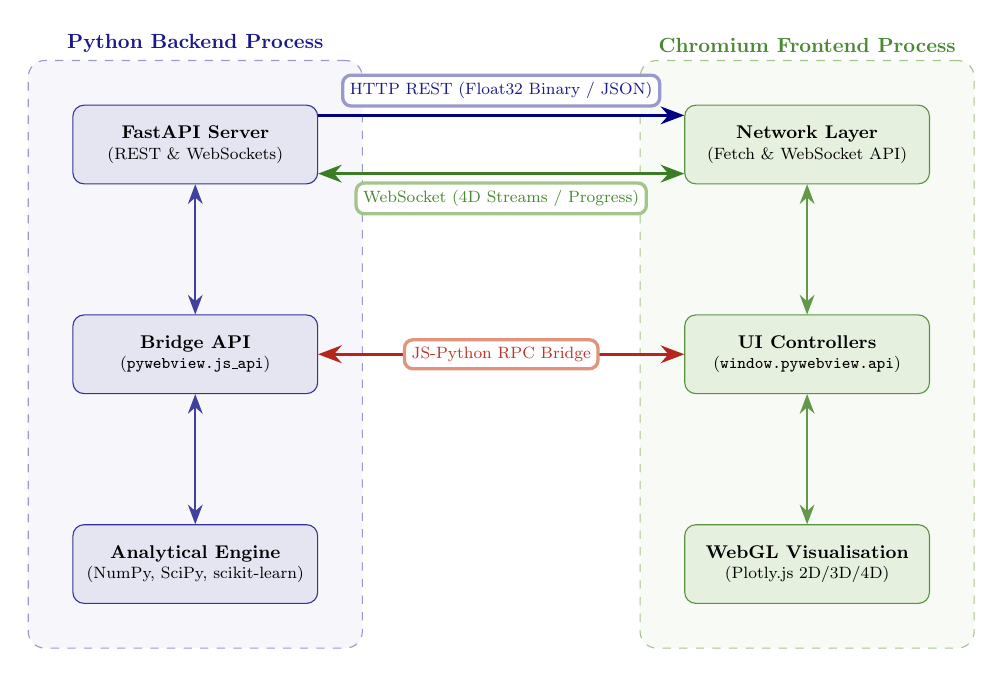
\begin{tikzpicture}[
    scale=0.74, transform shape,
    box_backend/.style={rectangle, draw=NavyBlue!80, fill=NavyBlue!10, rounded corners=4pt, minimum width=4.2cm, minimum height=1.35cm, align=center, font=\small},
    box_frontend/.style={rectangle, draw=OliveGreen!80, fill=OliveGreen!10, rounded corners=4pt, minimum width=4.2cm, minimum height=1.35cm, align=center, font=\small},
    container_backend/.style={rectangle, draw=NavyBlue!40, dashed, rounded corners=6pt, inner sep=16pt, fill=NavyBlue!3},
    container_frontend/.style={rectangle, draw=OliveGreen!40, dashed, rounded corners=6pt, inner sep=16pt, fill=OliveGreen!3},
    title_backend/.style={font=\bfseries\normalsize, text=NavyBlue!90},
    title_frontend/.style={font=\bfseries\normalsize, text=OliveGreen!90},
    proto_blue/.style={font=\footnotesize, fill=white, inner sep=3.5pt, draw=NavyBlue!40, text=NavyBlue!90, rounded corners=3pt},
    proto_green/.style={font=\footnotesize, fill=white, inner sep=3.5pt, draw=OliveGreen!40, text=OliveGreen!90, rounded corners=3pt},
    proto_red/.style={font=\footnotesize, fill=white, inner sep=3.5pt, draw=BrickRed!40, text=BrickRed!90, rounded corners=3pt}
]
    % Backend Nodes (All Blue = Python Backend Process at x = 0)
    \node[box_backend] (fastapi) at (0, 0) {\textbf{FastAPI Server}\\[-1pt]\footnotesize (REST \& WebSockets)};
    \node[box_backend] (bridge_py) at (0, -3.6) {\textbf{Bridge API}\\[-1pt]\footnotesize (\texttt{pywebview.js\_api})};
    \node[box_backend] (engine) at (0, -7.2) {\textbf{Analytical Engine}\\[-1pt]\footnotesize (NumPy, SciPy, scikit-learn)};
    
    % Frontend Nodes (All Green = Chromium Frontend Process at x = 10.5)
    \node[box_frontend] (web_client) at (10.5, 0) {\textbf{Network Layer}\\[-1pt]\footnotesize (Fetch \& WebSocket API)};
    \node[box_frontend] (ui_ctrl) at (10.5, -3.6) {\textbf{UI Controllers}\\[-1pt]\footnotesize (\texttt{window.pywebview.api})};
    \node[box_frontend] (plotly) at (10.5, -7.2) {\textbf{WebGL Visualisation}\\[-1pt]\footnotesize (Plotly.js 2D/3D/4D)};

    % Intra-process connections (Backend: Blue)
    \draw[{Stealth[length=2.5mm]}-{Stealth[length=2.5mm]}, thick, draw=NavyBlue!75] (fastapi.south) -- (bridge_py.north);
    \draw[{Stealth[length=2.5mm]}-{Stealth[length=2.5mm]}, thick, draw=NavyBlue!75] (bridge_py.south) -- (engine.north);

    % Intra-process connections (Frontend: Green)
    \draw[{Stealth[length=2.5mm]}-{Stealth[length=2.5mm]}, thick, draw=OliveGreen!75] (web_client.south) -- (ui_ctrl.north);
    \draw[{Stealth[length=2.5mm]}-{Stealth[length=2.5mm]}, thick, draw=OliveGreen!75] (ui_ctrl.south) -- (plotly.north);

    % Containers (Backgrounds matching Process colors)
    \begin{scope}[on background layer]
        \node[container_backend, fit=(fastapi) (engine), label={[title_backend]above:Python Backend Process}] (bg_backend) {};
        \node[container_frontend, fit=(web_client) (plotly), label={[title_frontend]above:Chromium Frontend Process}] (bg_frontend) {};
    \end{scope}

    % Inter-process communication channels (Horizontal lines with protocol-matched colors)
    % 1. HTTP REST API (Blue = Data Provider)
    \draw[-{Stealth[length=3.0mm]}, very thick, draw=NavyBlue] 
        ([yshift=5mm]fastapi.east) -- node[proto_blue, above=4pt] {HTTP REST (Float32 Binary / JSON)} ([yshift=5mm]web_client.west);

    % 2. WebSockets (Green = Live Client Duplex Stream)
    \draw[{Stealth[length=3.0mm]}-{Stealth[length=3.0mm]}, very thick, draw=OliveGreen] 
        ([yshift=-5mm]fastapi.east) -- node[proto_green, below=4pt] {WebSocket (4D Streams / Progress)} ([yshift=-5mm]web_client.west);

    % 3. Native Bridge RPC (Red = Native Inter-Process RPC Bridge)
    \draw[{Stealth[length=3.0mm]}-{Stealth[length=3.0mm]}, very thick, draw=BrickRed] 
        (bridge_py.east) -- node[proto_red] {JS-Python RPC Bridge} (ui_ctrl.west);

\end{tikzpicture}
\caption{Client-server architecture of Seismic Viewer with dedicated communication channels.}
\label{fig:arch-overview}
\end{figure}

\bluerevised{The architecture divides tasks across three dedicated communication channels, balancing responsiveness and data transfer speed:
\begin{enumerate}
    \item \textbf{Native Bridge}: Connects the user interface with the Python runtime for desktop actions. When the window opens, pywebview exposes methods of the Python \texttt{Api} class to JavaScript via \texttt{window.pywebview.api}. Actions such as selecting files or opening dialogs call these methods directly without network delay.
    \item \textbf{HTTP REST Endpoints}: Handles data transfer between backend and frontend. Rather than embedding large datasets into HTML pages, the frontend requests catalogs asynchronously. Numerical coordinates are streamed as Float32 binary buffers via \texttt{/api/data/\{id\}/bin}, while catalog metadata and views are served with standard compression.
    \item \textbf{WebSockets}: Manages live updates and streaming during long calculations. When running temporal animations or clustering routines, the backend streams progress notifications and frame updates directly to the client over an open connection, updating the interface without page reloads.
\end{enumerate}
\Cref{tab:rest-api} lists the REST endpoints and WebSocket message types supported by the system.}

\begin{table}[htbp]
\centering
\caption{REST API endpoints and WebSocket message protocol.}
\label{tab:rest-api}
\footnotesize
\renewcommand{\arraystretch}{1.1}
\begin{tabularx}{\textwidth}{@{}l l >{\raggedright\arraybackslash}X@{}}
\toprule
\textbf{Protocol / Endpoint} & \textbf{Direction / Path} & \textbf{Description / Message Types} \\
\midrule
REST (\texttt{GET}) & \texttt{/api/data/\{session\_id\}} & Retrieve session data as GZip-compressed JSON \\
REST (\texttt{GET}) & \texttt{/api/data/\{session\_id\}/bin} & Retrieve numerical data as Float32 binary buffer \\
REST (\texttt{GET}) & \texttt{/viz/\{viz\_id\}} & Serve pre-rendered HTML visualisation page \\
\midrule
WebSocket & Client $\to$ Server & \texttt{ping}, \texttt{get\_cluster\_update}, \texttt{get\_structural\_planes}, \texttt{get\_animated\_clustering} \\
WebSocket & Server $\to$ Client & \texttt{pong}, \texttt{rpc\_response}, \texttt{progress} (broadcast messages) \\
\bottomrule
\end{tabularx}
\end{table}

\section{Backend Architecture}
\label{sec:backend}

\subsection{Application Entry Point \& Bridge Engine}
\label{sec:bridge}

Once the application is running, the \texttt{Api} module acts as the central coordinator. Whenever the user interacts with the interface, such as selecting a file (\texttt{select\allowbreak\_csv()}), loading a 3D view (\texttt{load\allowbreak\_view()}), or exporting results (\texttt{export\allowbreak\_clusters\allowbreak\_csv()}), the frontend sends a request directly to this coordinator.

\bluerevised{These requests include spatial analysis calculations on seismic events. To prevent blocking the graphical interface during execution, operations run on background workers using threads or process pools. The application sends progress updates from worker threads to the WebSocket event loop without conflicts.}

Since the calculations occur in the background, the application requires a mechanism to inform the user about the ongoing progress. The coordinator handles this requirement by continuously transmitting real-time updates back to the interface. This ensures the user is constantly provided with a responsive progress bar or status message, resulting in a fluid and stable user experience. These updates are broadcast through the WebSocket protocol.

\subsection{Session Store \& FastAPI Middleware}
\label{sec:session-store}

The system architecture requires a dedicated memory management layer to preserve state between user interactions and to serve data efficiently to the graphical frontend. This functionality is centralized within an internal configuration module (\texttt{core/config.py}), which orchestrates two separate in-memory caches: \texttt{\_data\_store} and \texttt{\_html\_store}.

The \texttt{\_data\_store} structure retains the raw numerical arrays and metadata associated with each active analytical session. To guarantee that the application maintains a stable memory profile even during extensive analytical workflows, this cache is strictly limited to 30 concurrent sessions. In parallel, the \texttt{\_html\_store} caches up to 15 pre-rendered graphical views, allowing the frontend to load complex tridimensional scenes instantaneously. Both structures implement a First-In, First-Out (FIFO) eviction policy. \bluerevised{To ensure safety during simultaneous operations, updates to these stores are synchronized, keeping application memory use low during long sessions.}

Positioned between this caching layer and the client interface, the FastAPI server deploys specific middleware to optimize network throughput. An important optimization is the automatic application of GZip compression for any outgoing data payload larger than 500 bytes. Compressing the data prior to transmission accelerates the rendering process, particularly when transferring datasets containing tens of thousands of seismic events.

\section{Frontend Architecture}
\label{sec:frontend}

\subsection{Single-Page Application \& UI/UX Design}
\label{sec:spa}

As illustrated in \Cref{fig:gui-hub}, the primary workflow begins at the landing screen (\subref{fig:start-page}). Here, the system exposes multiple data ingestion pathways, allowing researchers to import local csv files, query the INGV remote web services directly, or restore a previously interrupted session through local historical records.

\bluerevised{Once the imported dataset is validated, the software opens the visualization hub (\subref{fig:viz-hub}). This view provides menus to switch between the available display modes and clustering algorithms. In addition, it includes toggles to display extra data layers on the 3D map, such as seismic tomography, ground uplift, and monitoring stations.}

\bluerevised{The 3D graphics pipeline delegates rendering to WebGL through Plotly.js. To preserve context during updates, the system retains the view angle and zoom level selected by the user. This prevents the camera from resetting when new data arrives, maintaining smooth interaction (\Cref{sec:challenge-camera}).}

\begin{figure}[H]
\centering
\begin{subfigure}{0.48\textwidth}
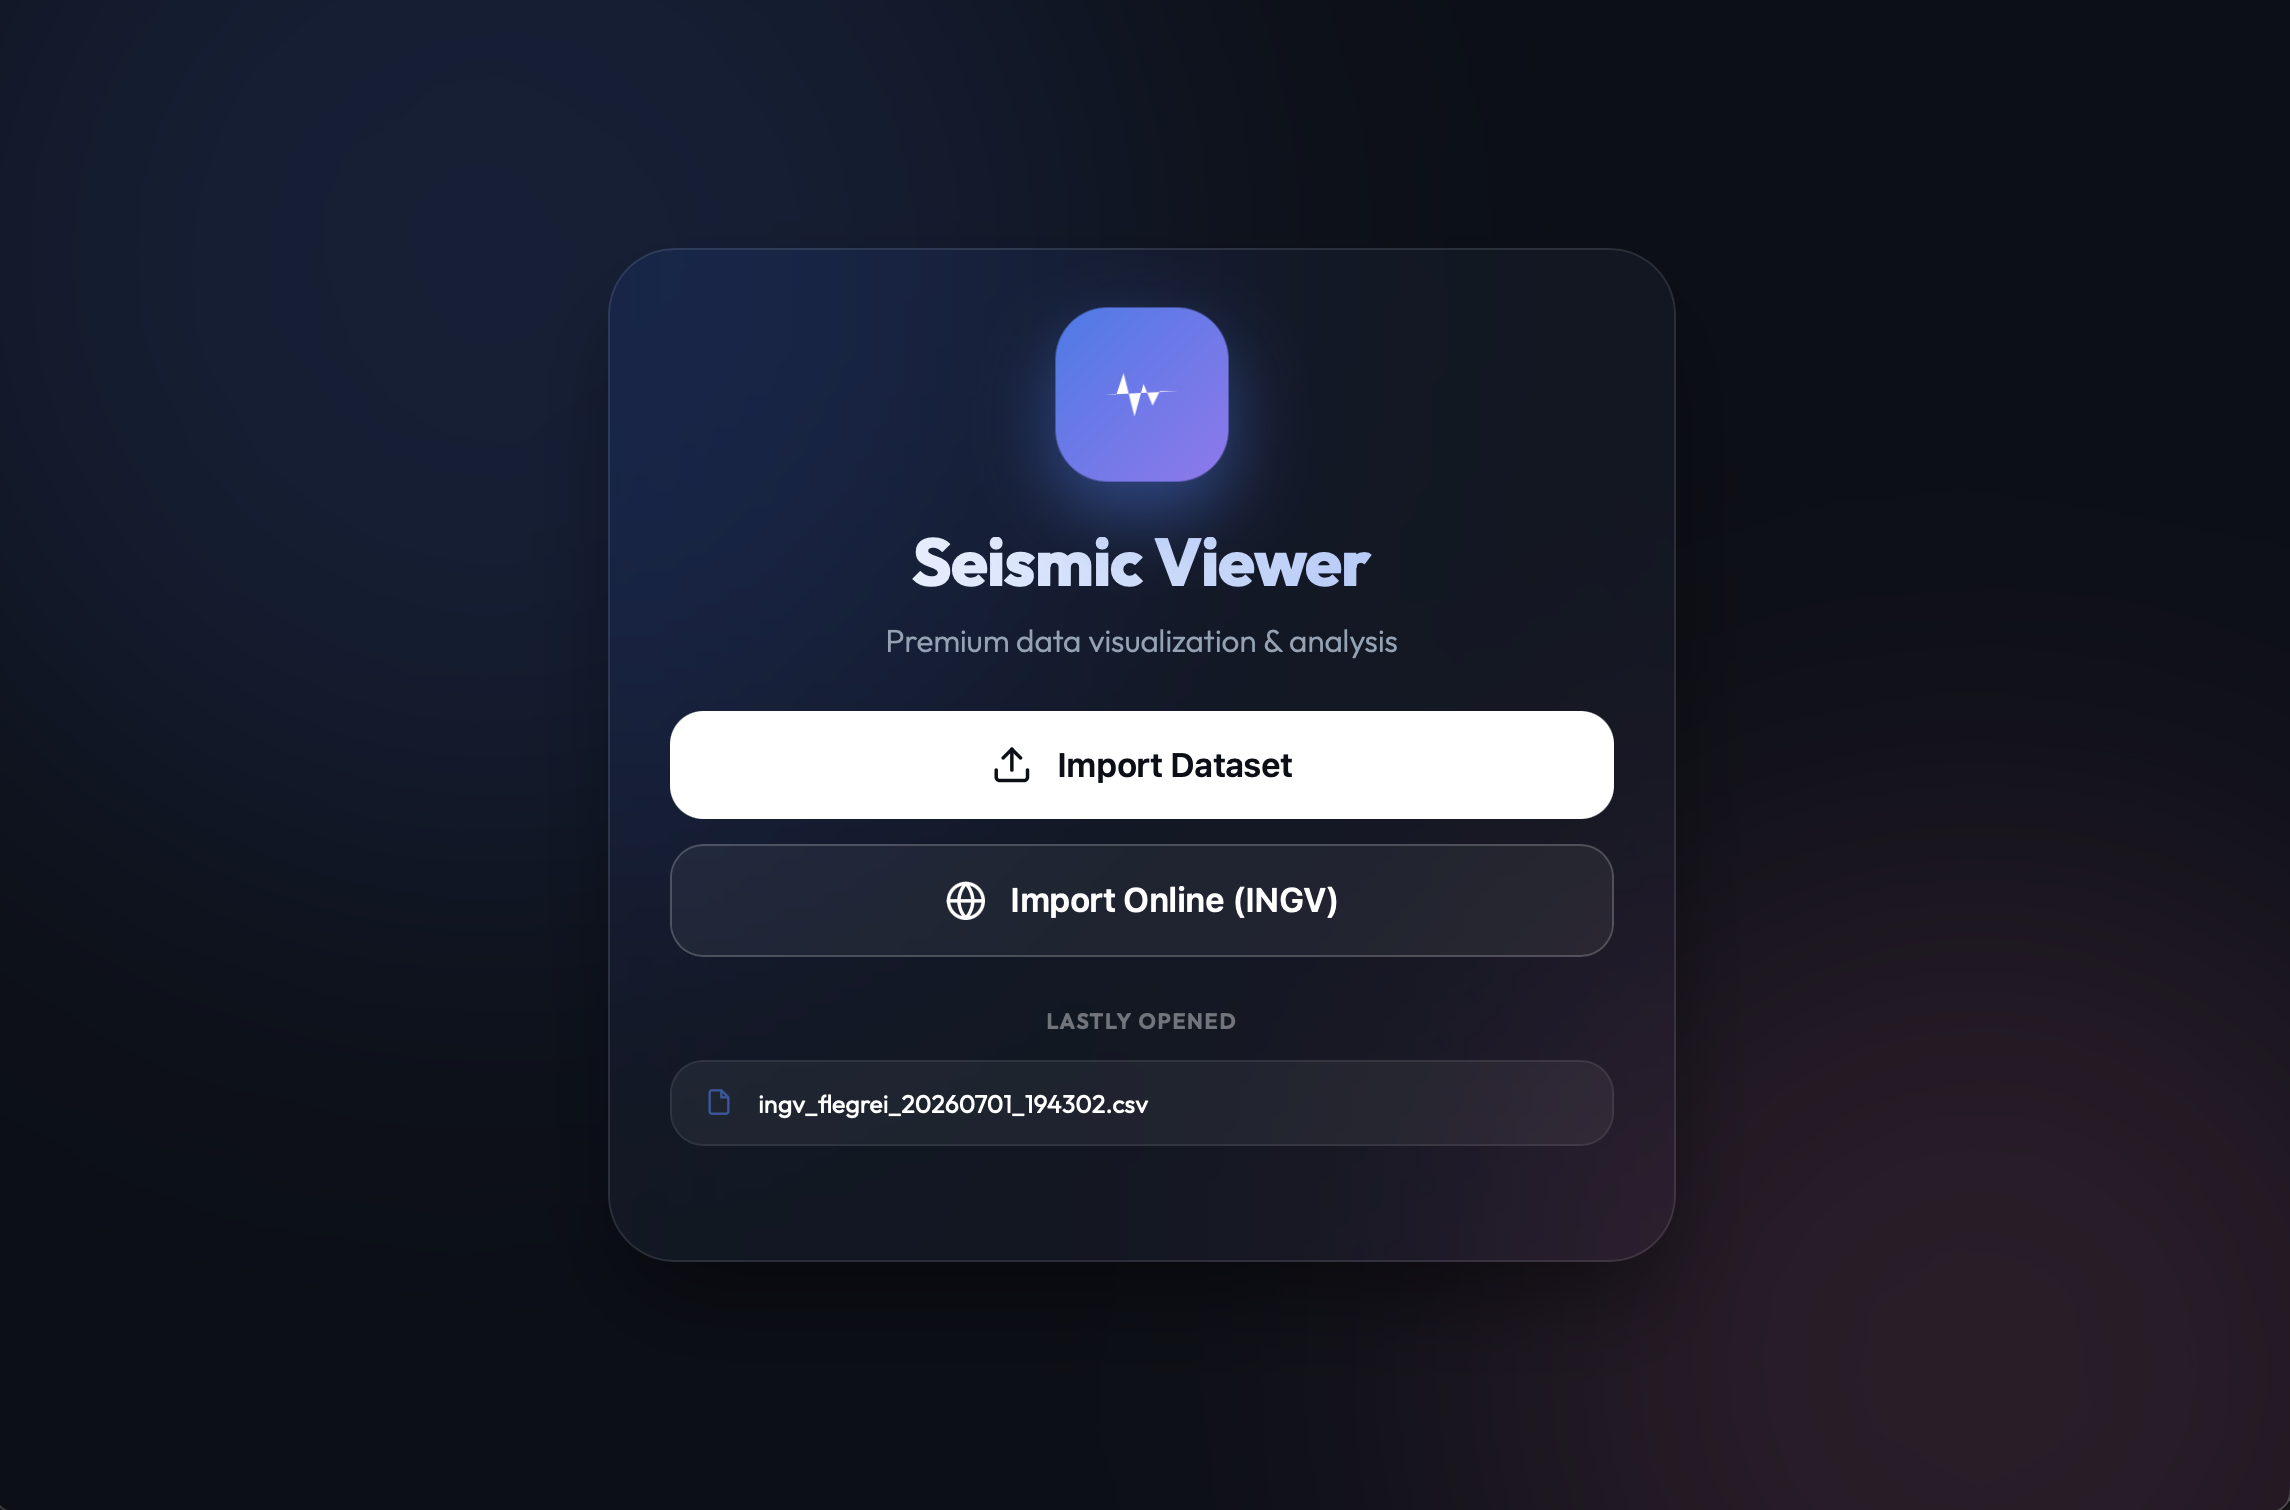
\includegraphics[width=\textwidth]{images/start_page.png}
\caption{File Picker view.}
\label{fig:start-page}
\end{subfigure}\hfill
\begin{subfigure}{0.48\textwidth}
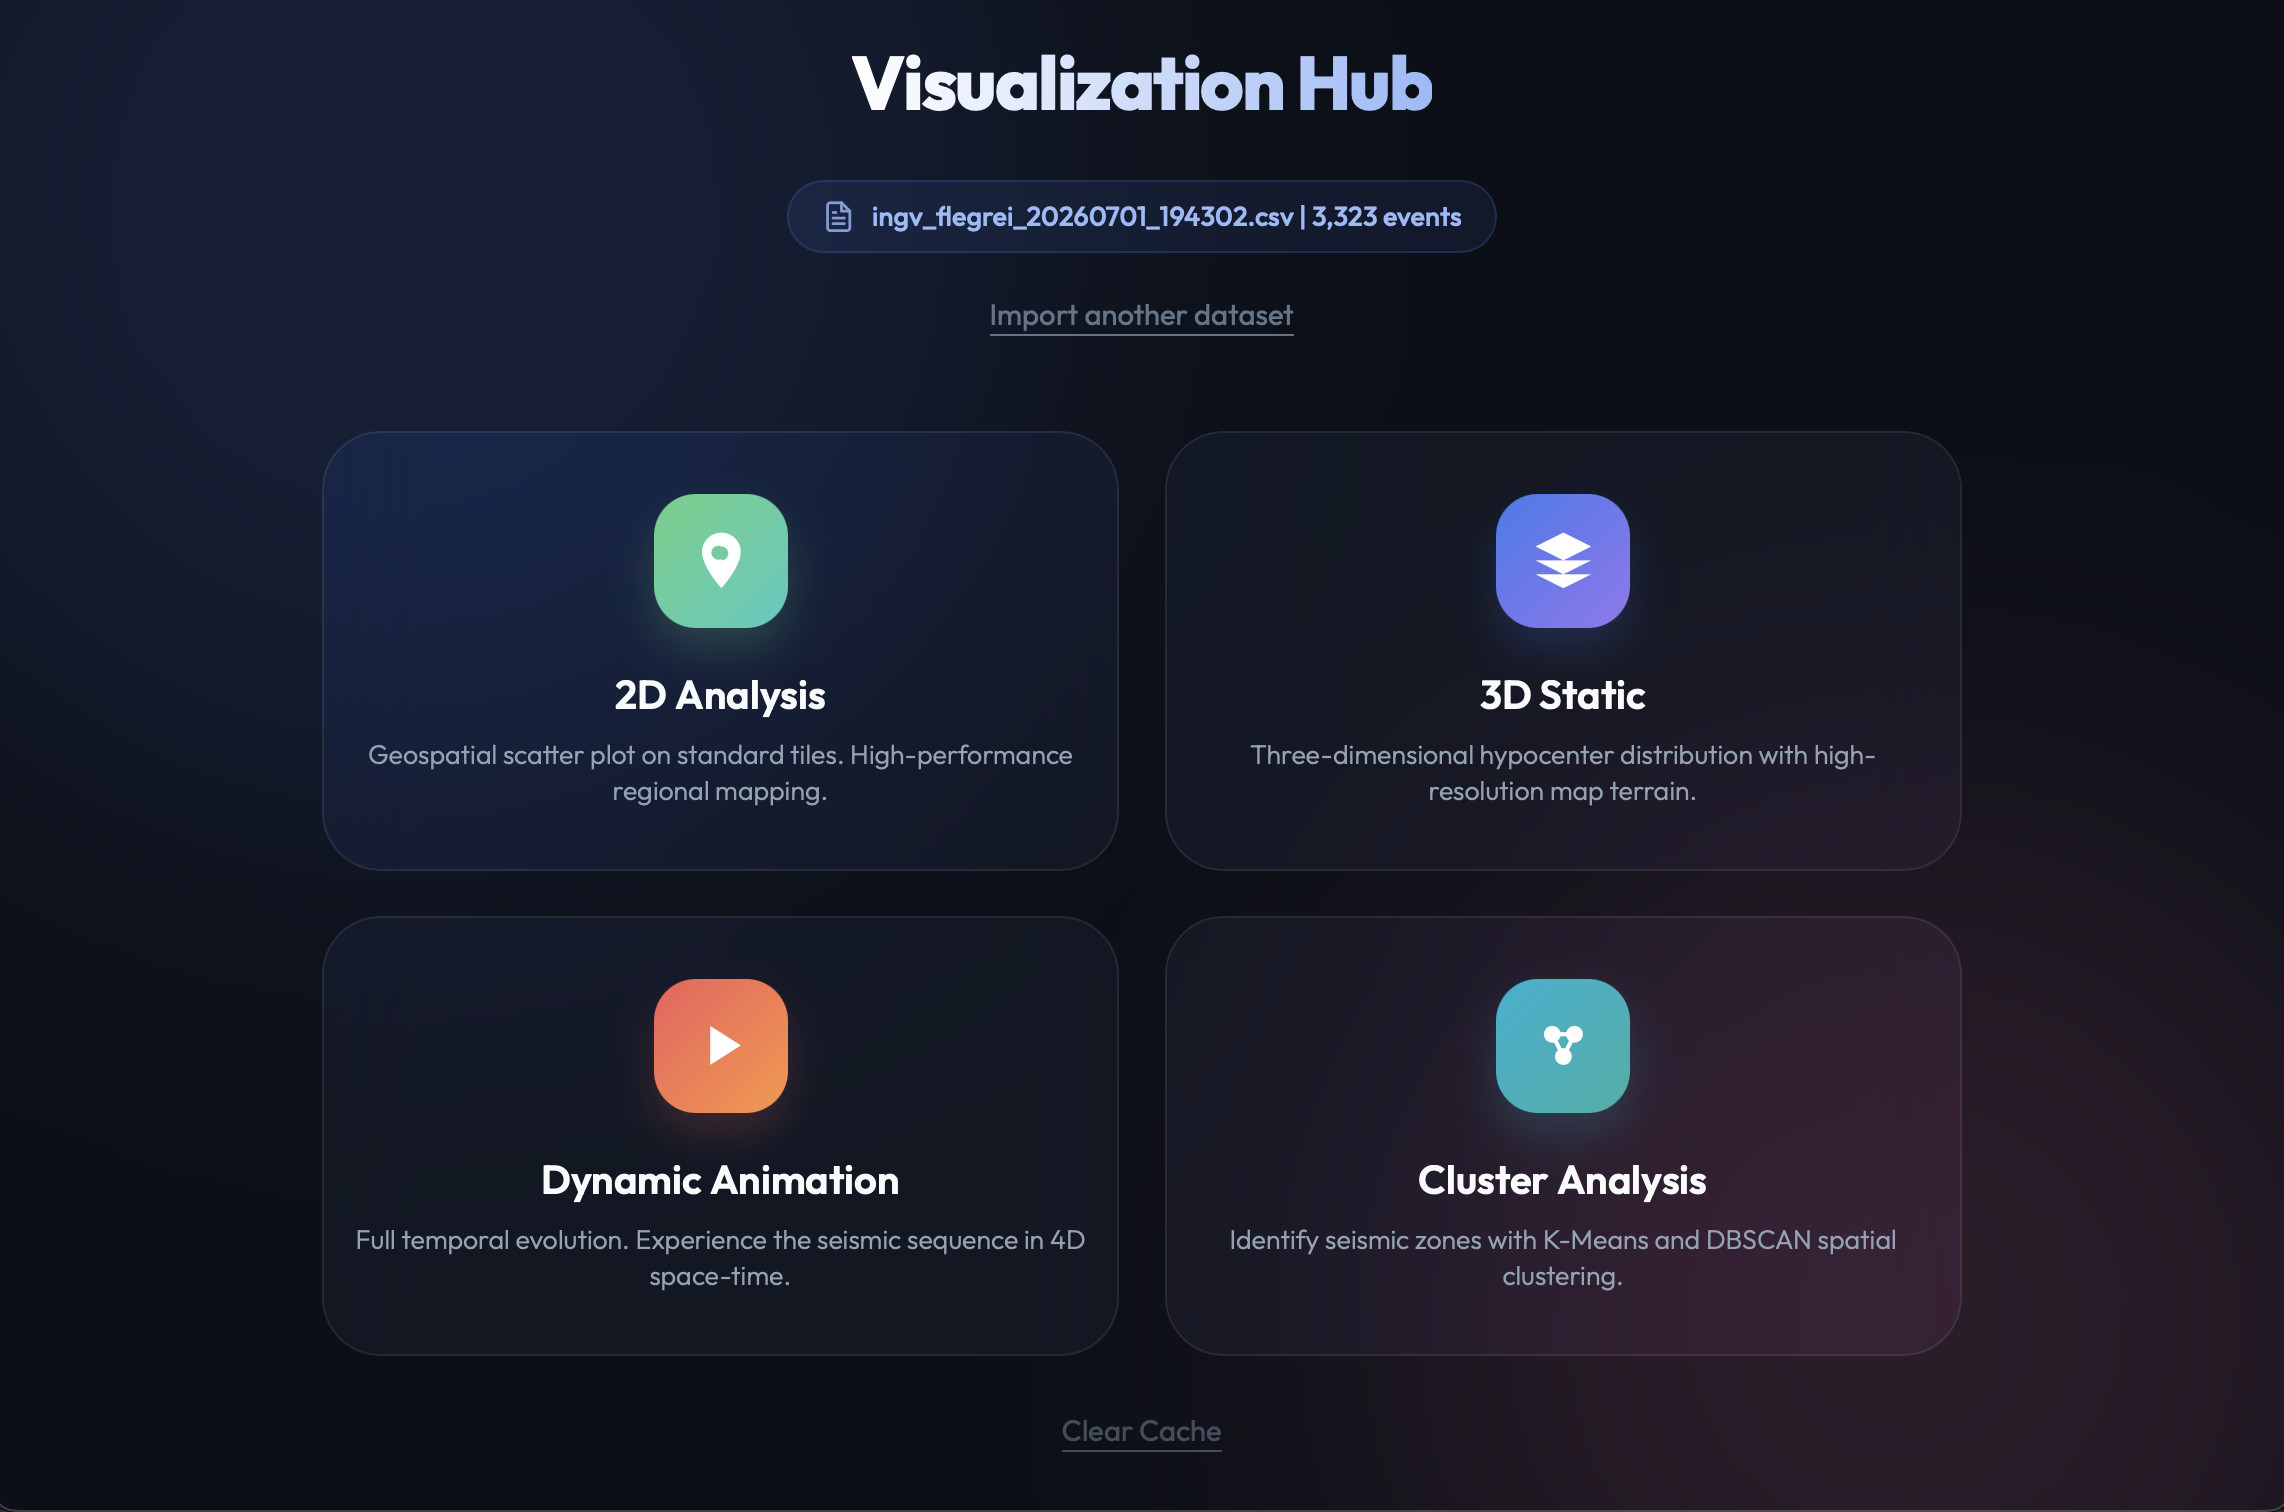
\includegraphics[width=\textwidth]{images/visualization_hub.png}
\caption{Visualisation Hub with mode selection.}
\label{fig:viz-hub}
\end{subfigure}
\caption{The Seismic Viewer single-page application structure, showing initial data loading (\subref{fig:start-page}) and the multi-mode analytical selection hub (\subref{fig:viz-hub}).}
\label{fig:gui-hub}
\end{figure}

\section{Data Flow Pipeline and Protocols}
\label{sec:dataflow}
\label{sec:protocols}

\bluerevised{To manage data processing and rendering, Seismic Viewer divides operations between backend services and the frontend client. On the backend, the system handles data loading, validation, and mathematical calculations. As shown in \Cref{fig:dataflow}, the pipeline begins by importing CSV data or querying the INGV API. This data is cleaned and loaded. Visual pre-computations prepare coordinate structures before the engine executes the selected algorithm. Finally, results are stored in the internal caches and rendered in HTML.}

\begin{figure}[H]
\centering
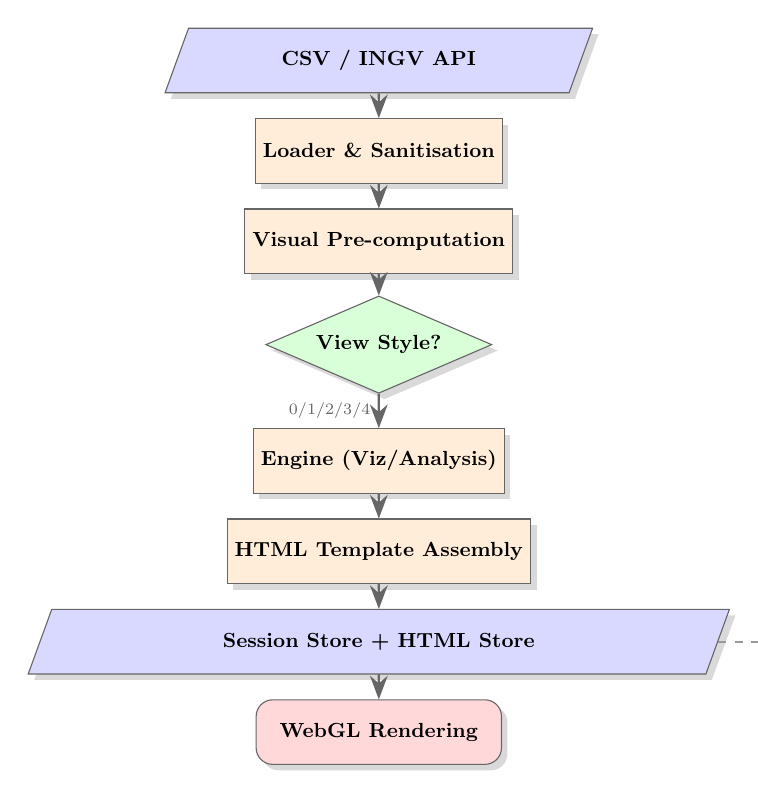
\begin{tikzpicture}[node distance=1.4cm, auto, scale=0.82, transform shape]
    \node (input) [io] {CSV / INGV API};
    \node (loader) [process, below of=input] {Loader \& Sanitisation};
    \node (precomp) [process, below of=loader] {Visual Pre-computation};
    \node (decision) [decision, below of=precomp, yshift=-0.2cm] {View Style?};
    \node (engine) [process, below of=decision, yshift=-0.4cm] {Engine (Viz/Analysis)};
    \node (template) [process, below of=engine] {HTML Template Assembly};
    \node (store) [io, below of=template] {Session Store + HTML Store};
    \node (render) [startstop, below of=store] {WebGL Rendering};

    \draw [arrow] (input) -- (loader);
    \draw [arrow] (loader) -- (precomp);
    \draw [arrow] (precomp) -- (decision);
    \draw [arrow] (decision) -- node[left, font=\scriptsize] {0/1/2/3/4} (engine);
    \draw [arrow] (engine) -- (template);
    \draw [arrow] (template) -- (store);
    \draw [arrow] (store) -- (render);
    \begin{pgfinterruptboundingbox}
    \draw [dashedarrow] (store.east) -- ++(2.4,0) node[right, font=\scriptsize, text width=3.2cm] {Binary Float32 buffer via \texttt{/api/data/\{id\}/bin}};
    \end{pgfinterruptboundingbox}
\end{tikzpicture}
\caption{Linear data pipeline from input parsing to WebGL drawing.}
\label{fig:dataflow}
\end{figure}

Once the backend processing is complete, the frontend retrieves the data through the defined REST API and WebSocket endpoints (\Cref{tab:rest-api}). The frontend dynamically renders the 3D scene using WebGL via the Plotly.js library. Continuous status updates, real-time recalculations, and filtering commands are exchanged over the WebSocket channel, ensuring the interface remains fully interactive without needing page reloads.

\begin{figure}[htbp]
\centering
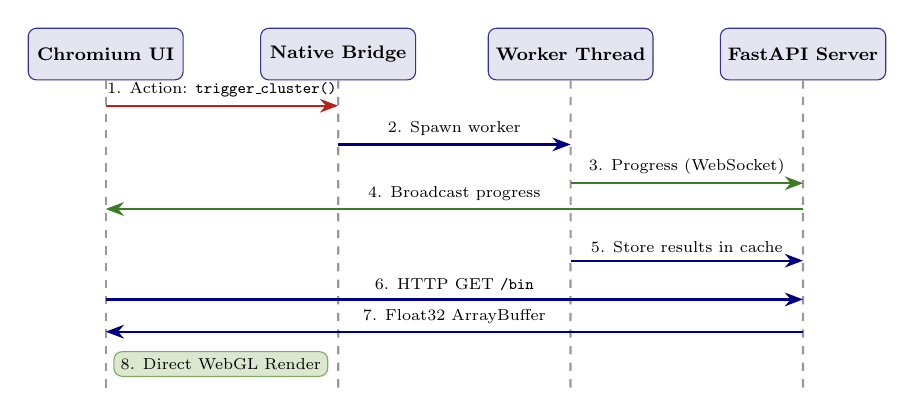
\begin{tikzpicture}[scale=0.82, transform shape,
    lifeline/.style={draw=black!40, dashed, thick},
    msg/.style={-Stealth, thick},
    actor/.style={rectangle, draw=NavyBlue!80, fill=NavyBlue!10, rounded corners=3pt, minimum width=2.4cm, minimum height=0.8cm, font=\footnotesize\bfseries, align=center}
]
    \node[actor] (ui) at (0, 0) {Chromium UI};
    \node[actor] (bridge) at (3.6, 0) {Native Bridge};
    \node[actor] (worker) at (7.2, 0) {Worker Thread};
    \node[actor] (fastapi) at (10.8, 0) {FastAPI Server};

    \draw[lifeline] (ui) -- (0, -5.2);
    \draw[lifeline] (bridge) -- (3.6, -5.2);
    \draw[lifeline] (worker) -- (7.2, -5.2);
    \draw[lifeline] (fastapi) -- (10.8, -5.2);

    \draw[msg, draw=BrickRed] (0, -0.8) -- node[above, font=\scriptsize] {1. Action: \texttt{trigger\_cluster()}} (3.6, -0.8);
    \draw[msg, draw=NavyBlue] (3.6, -1.4) -- node[above, font=\scriptsize] {2. Spawn worker} (7.2, -1.4);
    \draw[msg, draw=OliveGreen] (7.2, -2.0) -- node[above, font=\scriptsize] {3. Progress (WebSocket)} (10.8, -2.0);
    \draw[msg, draw=OliveGreen] (10.8, -2.4) -- node[above, font=\scriptsize] {4. Broadcast progress} (0, -2.4);
    \draw[msg, draw=NavyBlue] (7.2, -3.2) -- node[above, font=\scriptsize] {5. Store results in cache} (10.8, -3.2);
    \draw[msg, draw=NavyBlue] (0, -3.8) -- node[above, font=\scriptsize] {6. HTTP GET \texttt{/bin}} (10.8, -3.8);
    \draw[msg, draw=NavyBlue] (10.8, -4.3) -- node[above, font=\scriptsize] {7. Float32 ArrayBuffer} (0, -4.3);
    \node[fill=OliveGreen!15, draw=OliveGreen!60, rounded corners=3pt,
          font=\scriptsize, inner sep=3pt, anchor=west]
          at (0.12, -4.8) {8. Direct WebGL Render};
\end{tikzpicture}
\caption{Sequence diagram of asynchronous execution and non-blocking streaming pipeline.}
\label{fig:seq-diagram}
\end{figure}

\subsection{Binary Data Transfer Protocol}
\label{sec:binary-protocol}

To eliminate JSON parsing overhead during large catalog transfers, the backend packs numerical coordinates into a contiguous Float32 buffer (\texttt{/api/data/\{id\}/bin}) structured as: header \texttt{[event\_count, cluster\_count]} followed sequentially by arrays for longitude, latitude, magnitude, depth, \texttt{dates\_num}, and cluster labels ($C$ floats).

\begin{table}[htbp]
\centering
\caption{Binary buffer layout (Float32).}
\label{tab:binary-layout}
\footnotesize
\renewcommand{\arraystretch}{1.1}
\begin{tabular}{@{}l l | l l@{}}
\toprule
\textbf{Offset} & \textbf{Content} & \textbf{Offset} & \textbf{Content} \\
\midrule
0 (2 floats) & Header: \texttt{[N, C]} & $2+3N$ ($N$ floats) & Depth array \\
2 ($N$ floats) & Longitude array & $2+4N$ ($N$ floats) & Dates\_num array \\
$2+N$ ($N$ floats) & Latitude array & $2+5N$ ($C$ floats) & Cluster labels (if present) \\
$2+2N$ ($N$ floats) & Magnitude array & & \\
\bottomrule
\end{tabular}
\end{table}

\bluerevised{On the frontend, decoding via JavaScript's \texttt{Float32Array} directly over an \texttt{ArrayBuffer} completes in a few milliseconds even for large datasets, reducing transfer volume by approximately 80\% and avoiding JSON parsing delays.}

\section{Threading and Concurrency Model}
\label{sec:threading}

\begin{figure}[htbp]
\centering
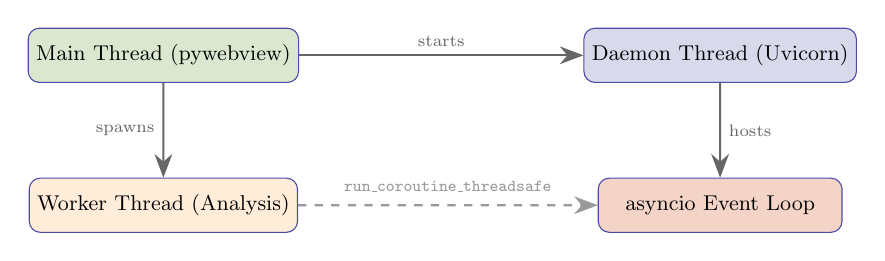
\begin{tikzpicture}[node distance=1.5cm and 4.2cm, scale=0.86, transform shape]
    \node[module, minimum width=3.6cm, fill=OliveGreen!15] (main) {Main Thread (pywebview)};
    \node[module, minimum width=3.6cm, fill=NavyBlue!15, right=4.2cm of main] (uvicorn) {Daemon Thread (Uvicorn)};
    \node[module, minimum width=3.6cm, fill=orange!15, below=1.4cm of main] (worker) {Worker Thread (Analysis)};
    \node[module, minimum width=3.6cm, fill=BrickRed!15, below=1.4cm of uvicorn] (asyncio) {asyncio Event Loop};

    \draw[arrow] (main) -- node[above, font=\scriptsize] {starts} (uvicorn);
    \draw[arrow] (main) -- node[left, font=\scriptsize] {spawns} (worker);
    \draw[arrow] (uvicorn) -- node[right, font=\scriptsize] {hosts} (asyncio);
    \draw[dashedarrow] (worker) -- node[above=2pt, font=\scriptsize\ttfamily] {run\_coroutine\_threadsafe} (asyncio);
\end{tikzpicture}
\caption{Concurrency hierarchy linking UI, server thread, and analysis worker threads.}
\label{fig:threading}
\end{figure}

The concurrency architecture separates responsibilities across the \textbf{Main Thread} (hosting pywebview and Chromium), the \textbf{Server Thread} (running the Uvicorn \cite{uvicorn} asyncio event loop), and on-demand \textbf{Worker Threads} handling view generation and clustering updates. For intensive multi-frame calculations (animated clustering and RANSAC+SVD plane tracking), the engine escalates to a \texttt{ProcessPoolExecutor} with up to 8 worker processes utilising shared memory initialisers to avoid array serialisation. \bluerevised{This concurrency model prevents lock contention during numerical loops, ensuring the interface remains smooth and responsive during intensive calculations.}

% ══════════════════════════════════════════════════════════════════════
% CHAPTER 4: DATA PROCESSING & GEOSPATIAL ENGINE
% ══════════════════════════════════════════════════════════════════════

\chapter{Data Processing and Geospatial Engine}
\label{ch:data}

This chapter details the processing pipeline that transforms raw seismic observations (whether sourced from local catalogs or remote web services) into optimized, GPU-ready structures for interactive 3D and 4D visualization.

\section{CSV Ingestion and Schema Detection}
\label{sec:csv-ingestion}

\revised{The \texttt{core/loader.py} module handles different formats through an ingestion pipeline that checks the header line for semicolon (\texttt{;}) or comma (\texttt{,}) delimiters, supporting European standards (INGV) as well as international formats (USGS, ISC). To avoid manual preprocessing, \texttt{core/config.py} defines an alias dictionary:}

\begin{lstlisting}[language=Python, caption={Flexible column schema definition in \texttt{core/config.py}.}, label={lst:schema}]
CSV_SCHEMA = {
    'time':  ['time', 'date', 'datetime', 'utc', 'time_utc', 'origintime'],
    'lat':   ['lat', 'latitude'],
    'lon':   ['lon', 'longitude'],
    'depth': ['depth', 'depth_km'],
    'mag':   ['mag', 'magnitude', 'md', 'ml', 'mw']
}
\end{lstlisting}

The ingestion pipeline identifies data columns by reading their headers. It ignores text case and removes any extra spaces. When a file contains unlabelled columns, the loader assumes a standard INGV column order based on their positions. Date processing is equally robust. The engine tests multiple known formats, covering both standard ISO timestamps and common European layouts.

\section{Data Sanitisation and Validation}
\label{sec:sanitisation}

Following ingestion, records undergo a four-stage sanitisation and validation sequence:
\begin{enumerate}
    \item \textbf{Spatial requirement check}: Rows missing latitude, longitude, or timestamps are discarded immediately.
    \item \textbf{Missing metadata flagging}: Catalogues occasionally omit depth or magnitude. \revised{In seismic analysis, estimating missing depths (such as using the mean value) is avoided because it groups points into artificial horizontal layers, distorting clustering and plane fitting results.} Rather than dropping these records (which removes spatial density) or imputing synthetic values, missing fields are flagged via boolean indicators (\texttt{depth\_is\_missing}, \texttt{mag\_is\_missing}) and assigned sentinel defaults (0.0~km depth and magnitude 0.1).
    \item \textbf{Geographic and depth bounds check}: The system excludes any event with mathematically invalid geographic coordinates (i.e., latitude outside the $\pm 90^\circ$ range or longitude outside the $\pm 180^\circ$ range). Additionally, it discards events with a depth falling outside the realistic geological range of $-10$~km to $800$~km, where negative values are specifically permitted to accommodate earthquakes occurring above sea level within mountains or volcanic edifices.
    \item \textbf{Chronological sorting \& future filtering}: Events with future timestamps are discarded, and the remaining catalog is sorted chronologically to optimize slicing.
\end{enumerate}

\section{Online Data Import: The INGV GOSSIP API}
\label{sec:online-import}

The \texttt{core/online\_importer.py} module interfaces directly with the INGV GOSSIP web service \cite{ingv}, providing high-resolution volcanic monitoring catalogues for Campi Flegrei, Vesuvius, and Ischia:

\begin{figure}[htbp]
\centering
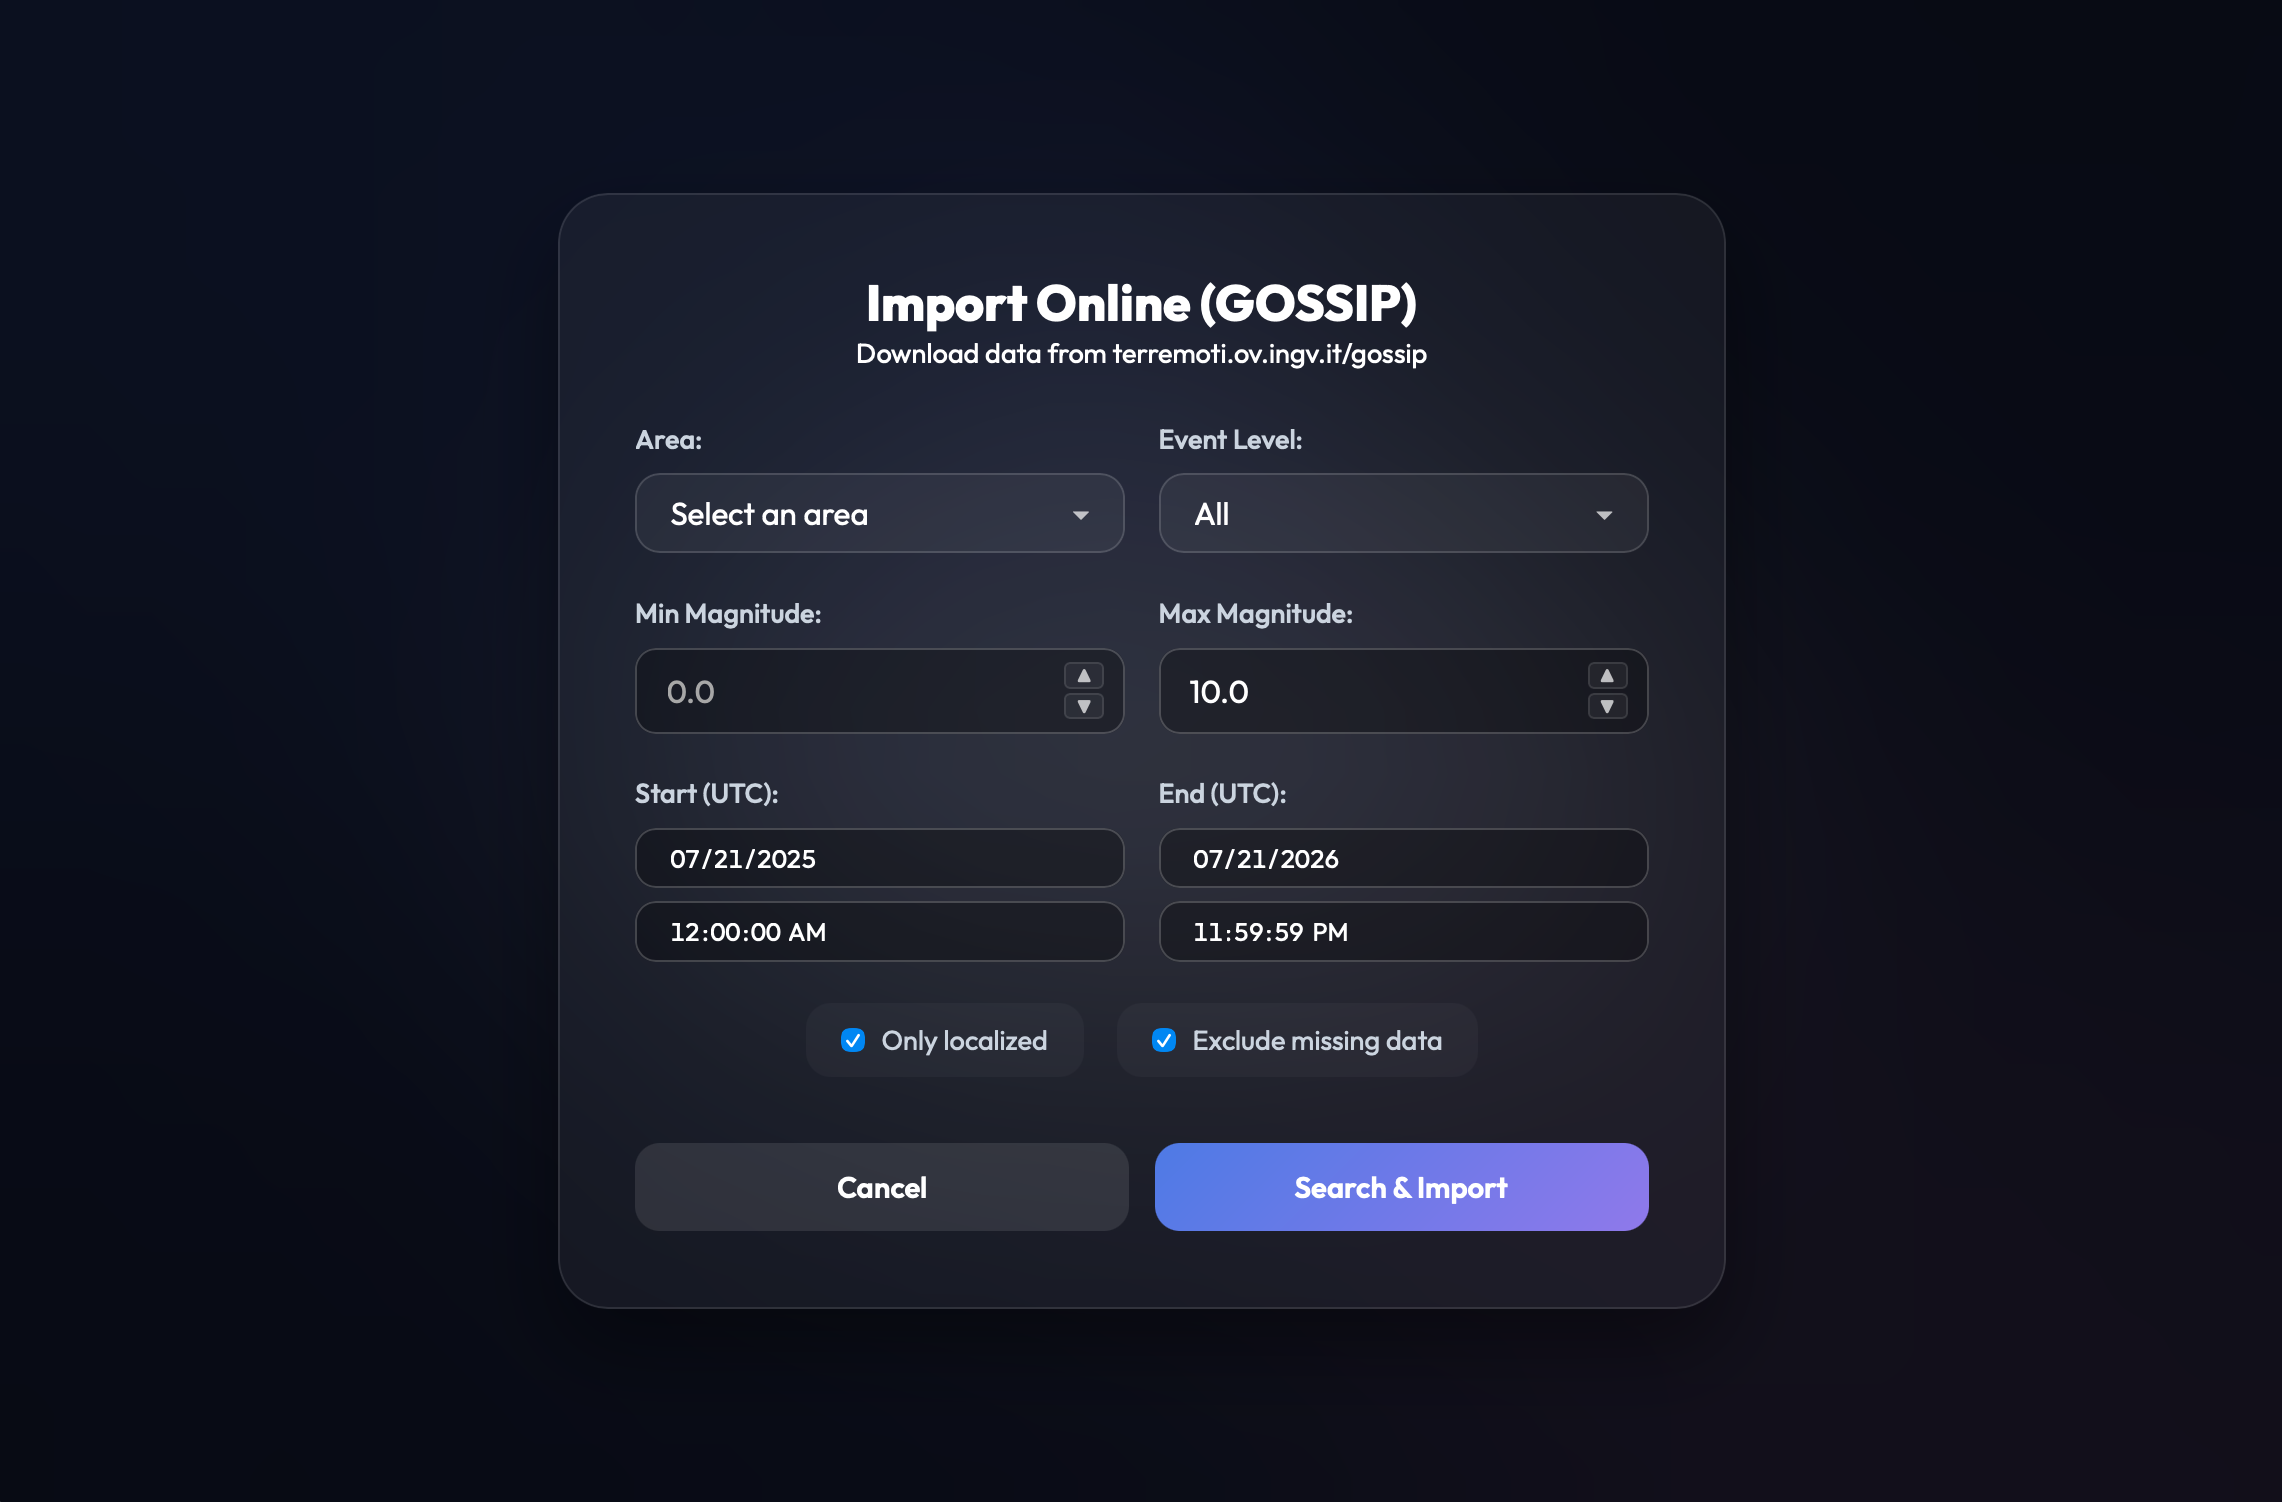
\includegraphics[width=1.0\textwidth]{images/online_import_ingv.png}
\caption{The INGV GOSSIP API import dialog for configuring network criteria, temporal bounds, and quality thresholds.}
\label{fig:online-import-ingv}
\end{figure}

The importer queries the official INGV GOSSIP web portal for each selected year (using the endpoint \texttt{https://\allowbreak terremoti.\allowbreak ov.\allowbreak ingv.\allowbreak it/\allowbreak gossip/\allowbreak <network>/\allowbreak <year>/\allowbreak events.json}). It downloads these annual JSON packets one by one to avoid network failures. As shown in \Cref{fig:online-import-ingv}, users can define the network target, the time span, the magnitude limits ($M_{\min}$ to $M_{\max}$), and the desired INGV revision quality (\texttt{automatico}, \texttt{rivisto}, or \texttt{bollettino}). Users can also apply additional filters to require confirmed coordinates (\texttt{located only}) or to drop records with incomplete information (\texttt{exclude missing}). Finally, the system converts these filtered records into a standard temporary CSV format and forwards them directly to the main ingestion pipeline.

\section{Geospatial Computations and Mesh Generation}
\label{sec:geospatial}

The 3D application visualises seismic activity over a base map retrieved from OpenStreetMap \cite{openstreetmap}. To accurately draw the earthquakes over this map, the software must convert the image pixel positions into standard geographic coordinates. The system solves this problem using an \textbf{inverse Mercator projection} \cite{snyder1987map} (implemented in \texttt{core/geo\_utils.py}). This mathematical operation translates pixel data into latitude and longitude, using NumPy \cite{numpy2020} arrays to guarantee fast execution:
\begin{equation}
    \lambda = \frac{x \cdot s}{t \cdot n} \cdot 360^\circ - 180^\circ, \quad
    \phi = \arctan\left(\sinh\left(\pi \left(1 - \frac{2 \cdot y \cdot s}{t \cdot n}\right)\right)\right) \cdot \frac{180^\circ}{\pi}
    \label{eq:mercator}
\end{equation}
In these equations, $\lambda$ and $\phi$ represent the resulting longitude and latitude in degrees. The values $x$ and $y$ correspond to the horizontal and vertical pixel coordinates on the screen. The variable $s$ is the current scaling factor of the map, while $t$ represents the fixed dimension of a single map tile (256 pixels). Lastly, $n$ is the total number of tiles across the map at the current zoom level $z$, calculated as $n = 2^z$.

\subsection{UTM Zone 33N to WGS84 Conversion}

Some advanced datasets, such as volcanic tomography grids, are originally provided in UTM Zone~33N coordinates instead of standard latitude and longitude. To ensure these layers align correctly with the rest of the 3D map, the \texttt{core/layer\_utils.py} module converts them using a Transverse Mercator inverse projection on the WGS84 ellipsoid:
\begin{equation}
    \phi = \phi_1 - \frac{N_1 \tan\phi_1}{R_1}\left(\frac{D^2}{2} - \frac{(5 + 3T_1 + 10C_1 - 4C_1^2 - 9e'^2)D^4}{24}\right)
\end{equation}
Here, $\phi$ is the final converted latitude. The formula relies on several variables derived from the WGS84 ellipsoid model. Specifically, $\phi_1$ is the footprint latitude, $N_1$ is the prime vertical radius of curvature, and $R_1$ is the meridional radius of curvature at $\phi_1$. The parameter $D$ represents the scaled distance from the central meridian, calculated as $D = (E - 500{,}000) / (N_1 k_0)$, where $E$ is the UTM Easting coordinate and $k_0$ is the central scale factor. Finally, $T_1$, $C_1$, and $e'^2$ are standard geometric constants related to the Earth's eccentricity.

\subsection{Optimised Map Mesh and Caching Architecture}

Terrain generation operates via a five-stage sequence: (1) bounding box squaring for uniform axis resolution, (2) deterministic cache lookup via MD5 hashing of rounded geographic bounds, (3) OpenStreetMap tile downloading via Smopy \cite{smopy} on cache misses, (4) palette-indexed downsampling to $1024 \times 1024$~px (256 colours), and (5) grid transformation via \Cref{eq:mercator}. Meshes are cached both in RAM (\texttt{@lru\_cache(maxsize=4)}) and disk (\texttt{.pkl}), guaranteeing sub-millisecond retrieval on subsequent loads.

\section{Pre-computation and Memory Layout Transformation}
\label{sec:precomputation}
\label{sec:strip-data}
\label{sec:binary-streaming}

To ensure the 3D map remains fluid and responsive even with thousands of earthquakes, the software performs several calculations in advance (during the data loading phase) rather than while the user is interacting with the map. The \texttt{precompute\_visual\_data()} function handles two main tasks. First, it pre-renders tooltip strings in a single batch operation, so that the browser does not need to construct the text for pop-ups every time the mouse hovers over an event. Second, it converts calendar dates into normalised time metrics (days since the first earthquake), accelerating chronological color mapping.

\revised{The data pipeline converts raw CSV lines into contiguous NumPy numerical arrays (\texttt{numpy.ndarray}). This enables vectorised operations on coordinates, depths, and timestamps. To stream data to the client efficiently, arrays are converted to 32-bit floating-point values (\texttt{np.float32}) and transmitted as raw bytes via \texttt{tobytes()}, avoiding JSON encoding overhead.}

\revised{Embedding large amounts of earthquake data directly into an HTML file increases file size and causes the browser to lag. To prevent this, Seismic Viewer uses an asynchronous loading strategy. When the user requests a 3D view, the backend generates an HTML page containing the 3D environment, base terrain maps, and UI menus. Once the base map is displayed, the browser requests the earthquake points in the background via \texttt{/api/data/\{id\}/bin}. These points are delivered as a Float32 binary buffer and populated onto the map without blocking user interaction.}

% ══════════════════════════════════════════════════════════════════════
% CHAPTER 5: CLUSTERING & STRUCTURAL ANALYSIS ALGORITHMS
% ══════════════════════════════════════════════════════════════════════

\chapter{Clustering and Structural Analysis Algorithms}
\label{ch:algorithms}

This chapter formalises the algorithms used in Seismic Viewer's analytical engine, presenting their mathematical formulations and optimisation strategies.

\section{Coordinate Projection and Spatial Clustering Methods}
\label{sec:projection}
\label{sec:clustering-methods}

To compute distances for spatial clustering, spherical coordinates ($\lambda, \phi$) are converted into a local Cartesian coordinate system in kilometres $(x, y, z)_\text{km}$ centred at the dataset mean $(\lambda_0, \phi_0)$. This projection \cite{snyder1987map} is defined as:
\begin{equation}
    x = (\lambda - \lambda_0) \cdot K \cos(\phi_0), \quad
    y = (\phi - \phi_0) \cdot K, \quad
    z = z_\text{depth}
    \label{eq:projection}
\end{equation}
where $K = 111.32$~km/° represents the average length of one degree of latitude, and $z_\text{depth}$ represents the depth of each individual earthquake (measured as positive downwards).

\subsection{DBSCAN, MiniBatchKMeans, and Cylinder Partitioning}
\label{sec:dbscan-impl}
\label{sec:kmeans-impl}
\label{sec:cylinder-clustering}

Seismic Viewer implements three complementary clustering paradigms, building on machine learning techniques for seismic catalogue analysis \cite{bergen2019machine} and provided by the scikit-learn library \cite{pedregosa2011sklearn} or developed as custom extensions:
\begin{enumerate}
    \item \textbf{DBSCAN}: The density-based spatial clustering algorithm \cite{ester1996dbscan} (\texttt{DBSCAN}) isolates high-density seismogenic structures according to neighbourhood radius $\varepsilon_\text{km} = \varepsilon_\text{m}/1000$ and \texttt{MinSamples}. Points lacking sufficient density reachability are marked as noise (label $-1$).
    \item \textbf{MiniBatchKMeans}: For centroid partitioning, the MiniBatchKMeans variant \cite{lloyd1982kmeans} optimises $K$ clusters across random data subsets ($b=1024$), reducing iteration complexity from $O(NK)$ to $O(bK)$. To prevent outlier inclusion, a post-clustering distance filter reclassifies points exceeding $d_\text{max}$ from their centroid as noise:
    \begin{lstlisting}[language=Python, caption={Post-clustering distance filter for KMeans.}, label={lst:kmeans-filter}]
if method == 'kmeans' and max_dist > 0:
    max_d = max_dist / 1000.0
    for i in range(n_clusters):
        idx = (labels == i)
        dists = np.sqrt(np.sum((pts_km[idx] - centroids[i])**2, axis=1))
        display_labels[np.where(idx)[0][dists > max_d]] = -1
    \end{lstlisting}
    \item \textbf{Cylinder Partitioning}: To ensure stable cluster assignments during 4D temporal animations without colour swapping, the study volume is partitioned into a regular grid of vertical cylinders. Events are assigned to the nearest cylinder centroid via KDTree query. Cylinders accumulating more than 5 events constitute stable, depth-resolved clusters across frames.
\end{enumerate}

\begin{table}[htbp]
\centering
\caption{Comparison of spatial clustering approaches in Seismic Viewer.}
\label{tab:clustering-comparison}
\footnotesize
\renewcommand{\arraystretch}{1.15}
\begin{tabularx}{\textwidth}{@{}l >{\raggedright\arraybackslash}X >{\raggedright\arraybackslash}X >{\raggedright\arraybackslash}X@{}}
\toprule
\textbf{Property} & \textbf{DBSCAN} & \textbf{MiniBatchKMeans} & \textbf{Cylinder Partition} \\
\midrule
\textit{Cluster count / shape} & Automatic / Arbitrary & User-defined ($K$) / Spherical & Grid-dependent / Cylindrical \\
\addlinespace
\textit{Noise handling} & Native (label $-1$) & Distance threshold ($d_\text{max}$) & Density threshold ($\geq 5$ events) \\
\addlinespace
\textit{Primary use case} & Unknown structures, swarms & Fixed centroid tracking & 4D animation, fault plane tracking \\
\bottomrule
\end{tabularx}
\end{table}

\section{Automatic Parameter Tuning}
\label{sec:auto-tuning}

Parameter tuning is executed during \textit{Subcluster Analysis} to estimate parameters for unlocked clusters based on their spatial distribution. The system uses a geometric knee-detection procedure inspired by the Kneedle algorithm \cite{satopaa2011kneedle}, which detects the point of maximum curvature in a sorted distance or inertia curve.

\paragraph{DBSCAN Auto-$\varepsilon$.}
Density-based clustering depends on two parameters: the search radius $\varepsilon$ and the minimum number of points $k = \text{MinSamples}$. Because these parameters depend on each other, the analytical engine determines both automatically. First, the minimum sample threshold is computed from the dataset size $N$ as $k = \max(3, \lfloor \ln N \rfloor)$, allowing the density requirement to adapt to the data volume. Next, using a nearest neighbour search, the algorithm calculates the distance $d_i^{(k)}$ from each earthquake to its $k$-th closest neighbour. Sorting these distances in ascending order yields the $k$-distance curve, denoted as points $\mathbf{p}_i = (i, d_i^{(k)})$ for $i = 0, \dots, N-1$.

In spatial clustering theory, points belonging to seismic clusters exhibit lower distances, whereas boundary events and noise cause the curve to rise. The search radius $\varepsilon^*$ corresponds to the knee point of this curve, which marks the transition between cluster density and noise. To identify this point, the system constructs a line between the first point $\mathbf{p}_0 = (0, d_0^{(k)})$ and the last point $\mathbf{p}_{N-1} = (N-1, d_{N-1}^{(k)})$, defining the direction vector $\mathbf{v} = \mathbf{p}_{N-1} - \mathbf{p}_0$. The algorithm calculates the distance from each curve point $\mathbf{p}_i$ to the line and selects the index $i^*$ that maximizes this distance:
\begin{equation}
    i^* = \arg\max_{0 \le i < N} \left\| (\mathbf{p}_i - \mathbf{p}_0) - \left( \frac{(\mathbf{p}_i - \mathbf{p}_0) \cdot \mathbf{v}}{\|\mathbf{v}\|^2} \right) \mathbf{v} \right\|
    \label{eq:max-curvature}
\end{equation}
The search radius is assigned as $\varepsilon^* = d_{i^*}^{(k)}$, providing a parameter that separates earthquake clusters from background noise.

\paragraph{MiniBatchKMeans Auto-$K$.}
For centroid-based clustering, finding the number of clusters $K$ requires balancing group compactness against model complexity. The analytical engine evaluates values from $K=2$ to $K=\min(10, N)$, computing the clustering inertia $J(K) = \sum_{j=1}^K \sum_{\mathbf{x} \in C_j} \|\mathbf{x} - \bm{\mu}_j\|^2$ for each configuration. Plotting $J(K)$ against $K$ produces a decreasing curve. The cluster count $K^*$ is identified by applying the projection method described in \Cref{eq:max-curvature} to the inertia curve, locating the elbow point where adding clusters yields diminishing improvements in compactness.

\section{Structural Plane Fitting and Geometric Synthesis}
\label{sec:ransac-svd}
\label{sec:convex-hull}

To extract planar fault structures from earthquake distributions, Seismic Viewer uses a two-stage process combining Random Sample Consensus (RANSAC) \cite{fischler1981ransac} and Singular Value Decomposition (SVD) \cite{shakarji1998least}. RANSAC isolates points belonging to a plane while removing noise. SVD then computes the best-fitting plane across the identified inliers and evaluates the planarity of the structure.

\subsection{RANSAC Robust Plane Estimation}

Seismic earthquakes rarely form perfect planes and contain background events. Fitting a plane directly using least squares is skewed by outliers. RANSAC addresses this through an iterative consensus search. In each step, the algorithm samples three points $\{P_1, P_2, P_3\}$ and calculates a candidate normal vector:
\begin{equation}
    \vec{n}_\text{cand} = \frac{(P_2 - P_1) \times (P_3 - P_1)}{\|(P_2 - P_1) \times (P_3 - P_1)\|}
    \label{eq:ransac-normal}
\end{equation}
The algorithm counts how many points in the cluster lie within a distance threshold of this candidate plane. Points meeting this condition are classified as inliers. This process is repeated across iterations, and the candidate model with the largest inlier count and lowest residual error is selected as the consensus set.

\subsection{SVD Refinement and Strike/Dip Mechanics}

Although RANSAC removes outliers and isolates the inlier set, the candidate plane itself is defined by three sample points. To obtain the plane that accounts for all identified inliers, the engine applies Singular Value Decomposition (SVD).

The software computes the centroid $(\bar{x}, \bar{y}, \bar{z})$ of all $n$ inliers and centres the coordinates at the origin, constructing the data matrix $A \in \mathbb{R}^{n \times 3}$:
\begin{equation}
    A = \begin{bmatrix}
        x_1 - \bar{x} & y_1 - \bar{y} & z_1 - \bar{z} \\
        \vdots & \vdots & \vdots \\
        x_n - \bar{x} & y_n - \bar{y} & z_n - \bar{z}
    \end{bmatrix}
    = U \Sigma V^T
    \label{eq:svd}
\end{equation}
The decomposition factors $A$ into orthogonal vectors and singular values $\Sigma = \operatorname{diag}(\sigma_1, \sigma_2, \sigma_3)$, where $\sigma_1 \ge \sigma_2 \ge \sigma_3 \ge 0$. The singular vector corresponding to the smallest singular value $\sigma_3$ defines the normal vector $\vec{n}$ of the fitted plane.

Beyond determining the plane orientation, the singular values provide direct insight into the geometric shape of the cluster. In structural geology and point cloud processing, dimensionality metrics are classically defined on the eigenvalues $\lambda_1 \ge \lambda_2 \ge \lambda_3$ of the sample covariance matrix $C = \frac{1}{n-1} A^T A$ \cite{fernandez2005plane}, where planarity is given by $P_\text{cov} = (\lambda_2 - \lambda_3) / \lambda_1$. Because the covariance eigenvalues relate to the SVD singular values through $\lambda_i = \sigma_i^2 / (n-1)$, an equivalent formulation can be expressed using squared singular values. In Seismic Viewer, as a direct and computationally lightweight implementation choice, the analytical engine calculates the planarity score directly from the singular values without forming the covariance matrix or computing squares:
\begin{equation}
    P = \frac{\sigma_2 - \sigma_3}{\sigma_1}
    \label{eq:planarity}
\end{equation}
A high planarity score ($P \to 1$) indicates a planar fault segment, whereas a low score ($P \to 0$) denotes an isotropic or linear dispersion of seismic hypocentres.

To translate the normal vector $\vec{n} = [n_x, n_y, n_z]$ into standard geological angles, the vector is oriented upwards ($n_z \ge 0$) within the Cartesian elevation frame (where subterranean depth corresponds to $z \le 0$). Under this convention, the horizontal projection points along the azimuth of maximum downward slope. Trigonometric relations then compute the orientation of the fault:
\begin{align}
    \text{Dip}: \quad & \delta = \arccos(n_z) \cdot \frac{180^\circ}{\pi} \label{eq:dip} \\
    \text{Dip Direction}: \quad & \theta_\text{DD} = \text{atan2}(n_x, n_y) \bmod 360^\circ \label{eq:dip-dir} \\
    \text{Strike}: \quad & \phi_s = (\theta_\text{DD} - 90^\circ) \bmod 360^\circ \label{eq:strike}
\end{align}
The Dip measures the tilt angle relative to the horizontal plane, the Dip Direction indicates the azimuth of the downward slope, and the Strike defines the orientation of the horizontal fault line. For 3D visualisation, planes are rendered as triangulated grids along orthogonal basis vectors $\vec{u}$ and $\vec{v}$:
\begin{equation}
    \vec{u} = \begin{bmatrix} \sin(\phi_s) \\ \cos(\phi_s) \\ 0 \end{bmatrix}, \quad \vec{v} = \vec{u} \times \vec{n}
    \label{eq:basis-vectors}
\end{equation}
where $\vec{u}$ is the horizontal unit vector oriented along the strike azimuth, and $\vec{v}$ is the down-dip vector pointing along the maximum downward slope of the fault plane.

\section{Temporal Stability, Parallel Execution, and Complexity}
\label{sec:label-matching}
\label{sec:parallel}

Computing structural models across temporal sequences requires visual consistency and computational efficiency. This section describes the temporal tracking mechanism, the parallel execution model, and the computational complexity of the analytical engine.

\subsection{Temporal Stability via Global Label Matching}
\enlargethispage{4\baselineskip}

When running unsupervised clustering algorithms frame by frame during 4D animations, each time step evaluates an independent subset of seismic events. Because unsupervised algorithms assign cluster labels without historical context, the label of a fault structure can change between consecutive frames. In an animation, this causes colour changes, known as colour flickering, which prevents tracking how faults evolve over time.

To maintain colour continuity across frames, the engine uses a label matching algorithm. The system maintains an array recording the most recent label assigned to each earthquake. For every cluster detected in a new frame, the algorithm inspects the previous labels of its events and applies majority voting:
\begin{equation}
    L_\text{assigned} = \arg\max_k \sum_{j \in S_c} \mathbb{I}(\text{global\_map}[j] = k)
    \label{eq:majority-voting}
\end{equation}
where $S_c$ is a sample of indices from the cluster (bounded to 200 events), and $\mathbb{I}$ is the indicator function. If a cluster contains only new events without previous history, the algorithm assigns a new label. The assigned label is applied to colour the earthquakes in the active frame and saved in the global array so that subsequent frames reuse the same cluster identifier.

\subsection{Parallel Execution Architecture}

Calculating RANSAC inliers and SVD planes across animation frames involves separate mathematical steps for each time window. To prevent these calculations from slowing down the user interface, the backend distributes frame tasks across worker threads using a \texttt{ThreadPoolExecutor}. The coordinate array is stored once in shared memory, allowing worker threads to read coordinates directly without making copies. Furthermore, numerical routines in SciPy and NumPy release the Global Interpreter Lock during LAPACK SVD calls and distance calculations, enabling efficient parallel execution across CPU cores.

\subsection{Asymptotic Complexity Analysis}

\Cref{tab:complexity} summarizes the typical time and space complexity of each algorithm in the pipeline under the operational assumptions of low spatial dimensionality ($d=3$) and balanced tree structures. Under these conditions, spatial neighbour searches in DBSCAN use a KD-Tree index to achieve an expected query complexity of $O(N \log N)$, whereas unindexed searches or degenerate distributions require $O(N^2)$. MiniBatchKMeans scales with mini-batch size $b$, cluster count $K$, spatial dimension $d=3$, and iterations $I$. Plane fitting scales with the number of inliers per cluster, and label matching remains bounded by sampling.

\begin{table}[H]
\centering
\caption{Typical asymptotic time and space complexity of the analytical methods under 3D spatial indexing assumptions.}
\label{tab:complexity}
\scriptsize
\setlength{\tabcolsep}{2.5pt}
\renewcommand{\arraystretch}{0.90}
\begin{tabularx}{\textwidth}{@{}l l l >{\raggedright\arraybackslash}X@{}}
\toprule
\textbf{Algorithm / Method} & \textbf{Time Complexity} & \textbf{Space Complexity} & \textbf{Parameters \& Notation} \\
\midrule
DBSCAN (KD-Tree) & $O(N \log N)$ (expected) & $O(N)$ & $N$ events, $\varepsilon$ radius; worst case $O(N^2)$ without index \\
MiniBatchKMeans & $O(b \cdot K \cdot d \cdot I)$ & $O(b \cdot K)$ & $b=1024$ batch, $K$ centroids, $d=3$, $I$ iterations \\
Cylinder Partitioning & $O(N \log M)$ & $O(M + N)$ & $M$ grid cylinders ($60 \times 50$) \\
Knee-Detection Auto-Tuning & $O(N \log k + K_\text{max} \cdot b \cdot d)$ & $O(N)$ & Chord distance, $k$-NN ($k = \max(3, \lfloor \ln N \rfloor)$) \\
RANSAC + SVD Fitting & $O(I_\text{ransac} \cdot N_\text{cluster} + d^3)$ & $O(N_\text{cluster})$ & $I_\text{ransac}=100$, spatial dimension $d=3$ \\
Global Label Matching & $O(K \cdot \min(N_c, 200))$ & $O(N)$ & Majority voting with bounded sampling \\
\bottomrule
\end{tabularx}
\end{table}

% ══════════════════════════════════════════════════════════════════════
% CHAPTER 6: VISUALISATION MODES
% ══════════════════════════════════════════════════════════════════════

\chapter{Visualisation Modes}
\label{ch:visualisation}

Seismic Viewer provides four primary visualisation modes, each addressing a distinct analytical need. This chapter documents their implementation, rendering strategies, and integration with auxiliary geophysical data layers.

\section{2D Geospatial Map View}
\label{sec:view-2d}

The 2D view provides a plan-view representation of earthquake epicentres overlaid on OpenStreetMap \cite{openstreetmap} tiles, implemented through Plotly's map interfaces (\texttt{scatter\_map} and \texttt{scatter\_mapbox}). The map visualises seismic data using two distinct graphical layers:
\begin{itemize}
    \item \textbf{Scatter Markers}: Each earthquake is represented by a circular marker. The visual properties of these circles can be mapped to different physical parameters depending on analytical needs. By default, the size of the circle indicates the magnitude of the event (with a minimum size threshold to ensure micro-earthquakes remain visible), and the colour represents the hypocentral depth. These mappings are flexible, allowing users to visualise other variables, such as chronological progression. Users can interact with these markers by hovering over them to reveal detailed statistics.
    \item \textbf{Density Heatmap}: A spatial density layer that visually aggregates tightly clustered earthquakes. By rendering a continuous colour gradient over regions of high seismicity, this optional overlay allows researchers to identify active swarm locations and broader structural trends that might be difficult to perceive when analysing individual scatter points alone.
\end{itemize}

To explore the dataset, users can apply filters based on magnitude, depth, and date ranges using dedicated input fields located on the left-hand panel. All filtering operations are processed directly within the user's web browser. This approach avoids sending new requests to the main server, ensuring that the map updates promptly whenever a parameter is changed.

\begin{figure}[H]
\centering
\begin{subfigure}[t]{0.85\textwidth}
\centering
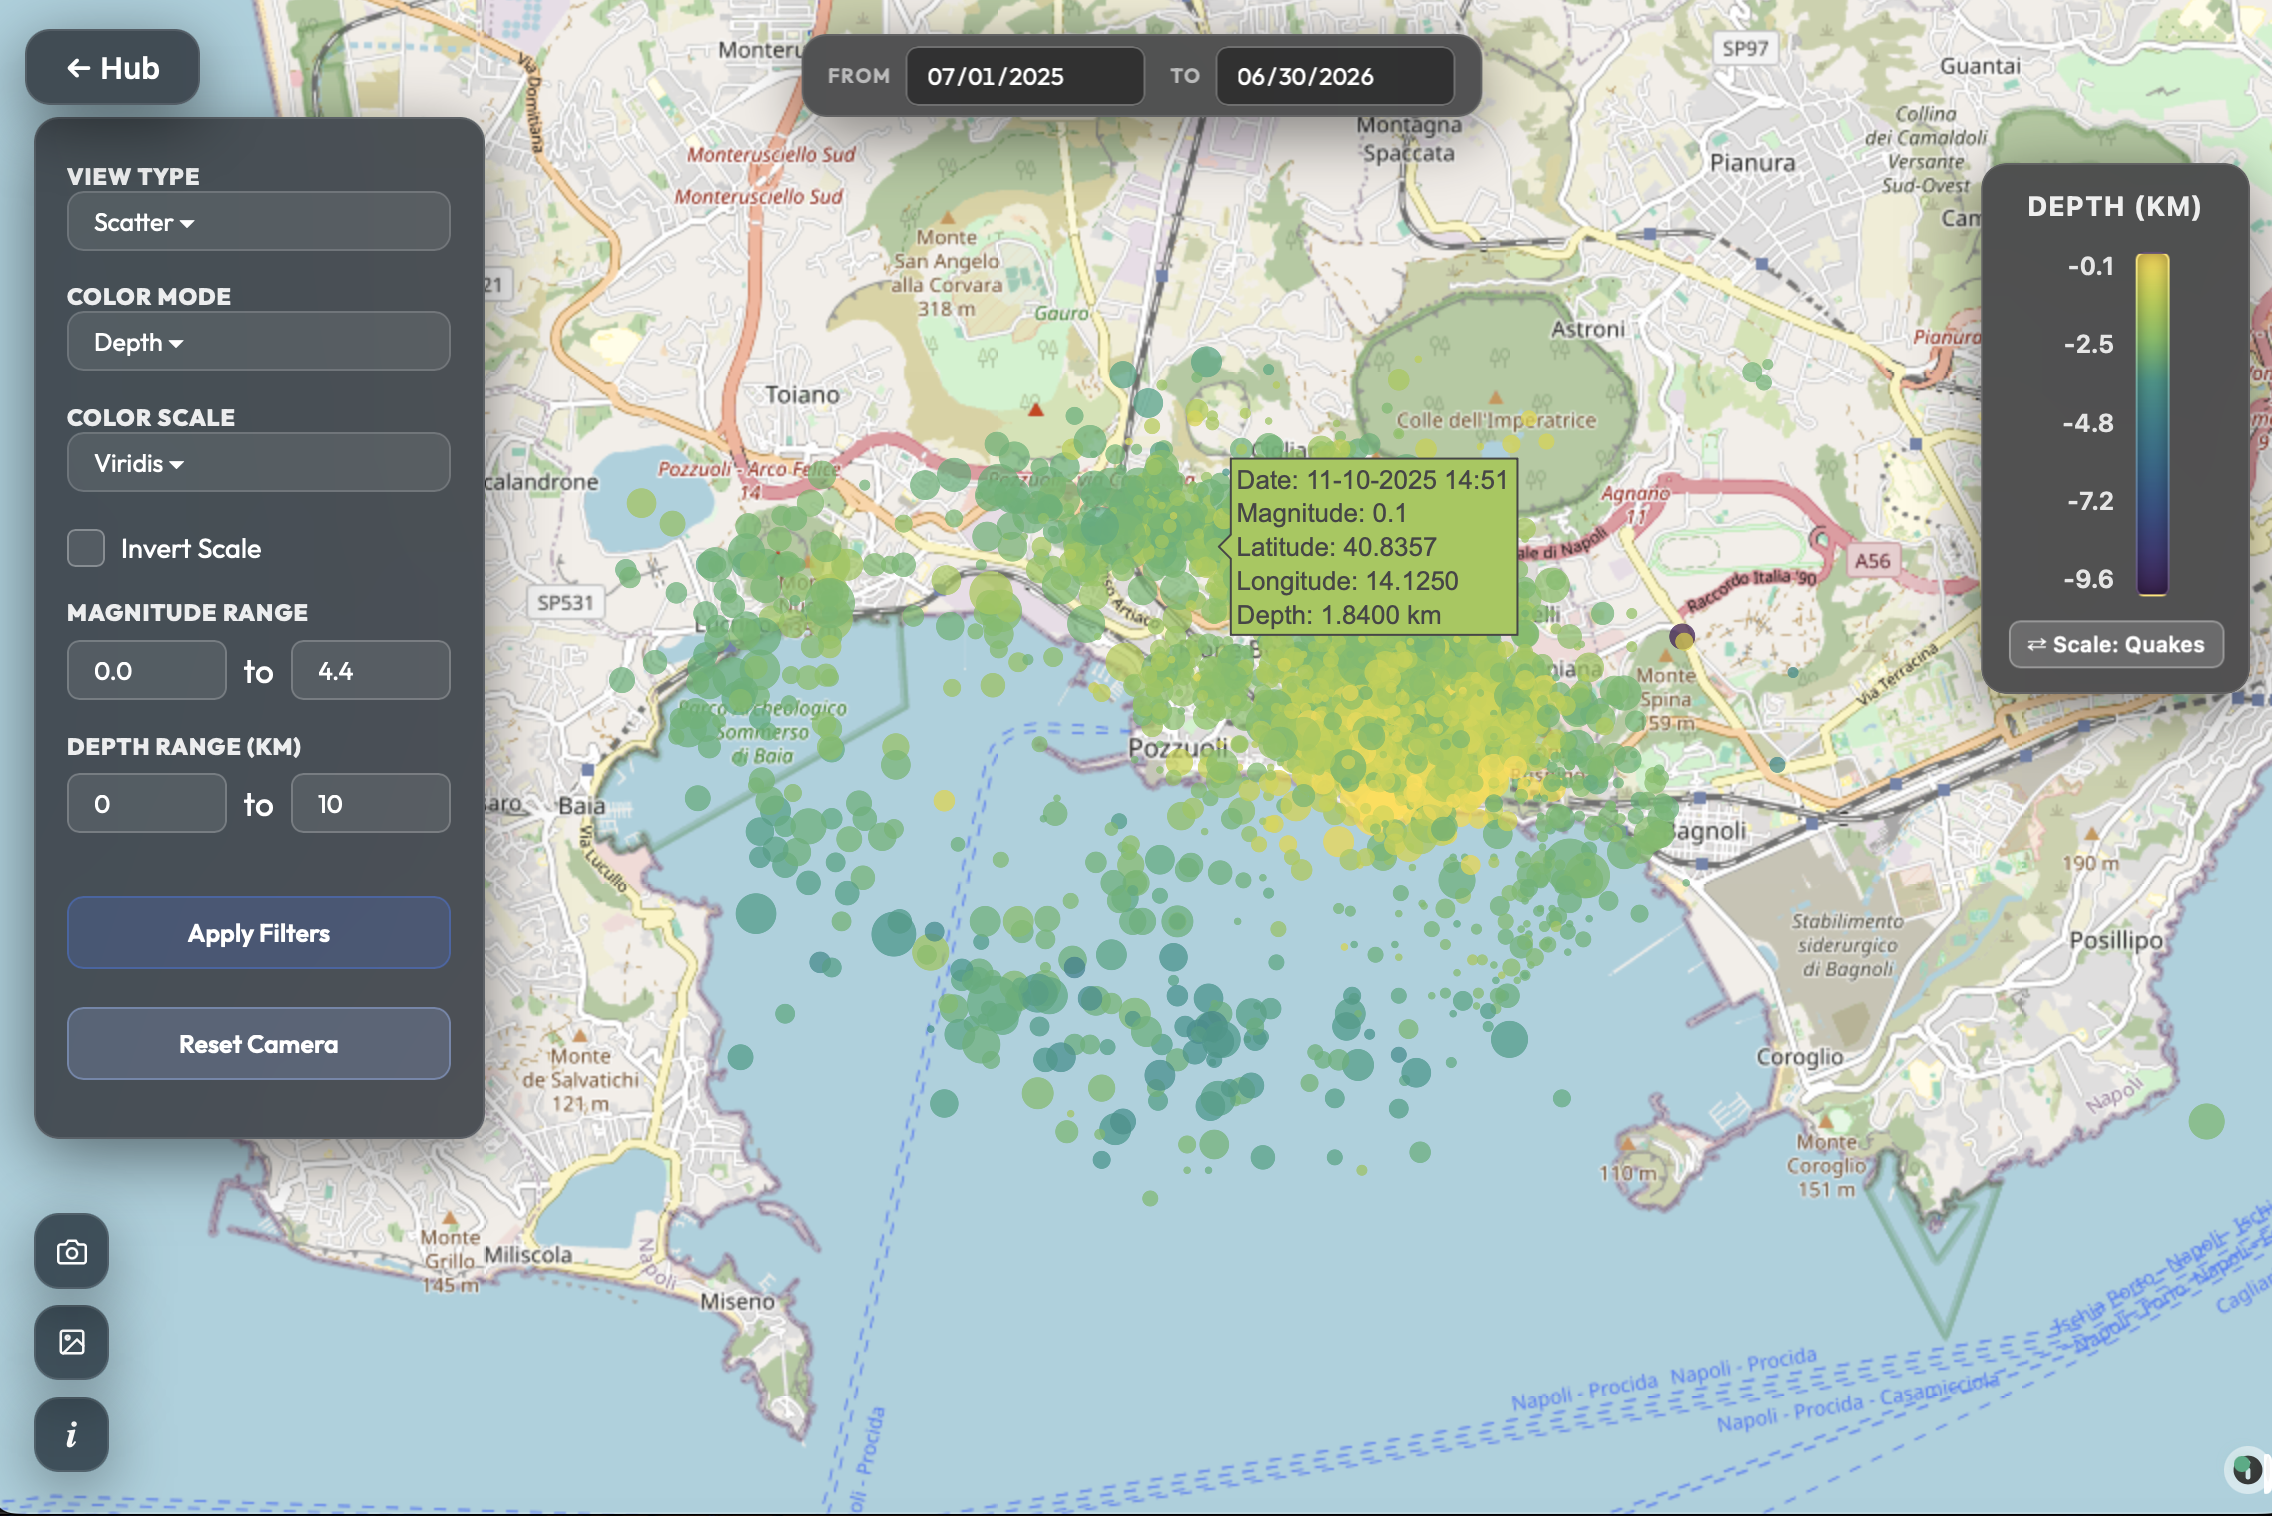
\includegraphics[width=\textwidth, height=0.66\textwidth]{images/2d_visualization.png}
\caption{The 2D base map showing earthquake locations. On the left panel, input fields allow the user to filter the data by magnitude, depth, and date.}
\label{fig:2d-viz}
\end{subfigure}
\end{figure}

\begin{figure}[H]
\ContinuedFloat
\centering
\begin{subfigure}[t]{0.85\textwidth}
\centering
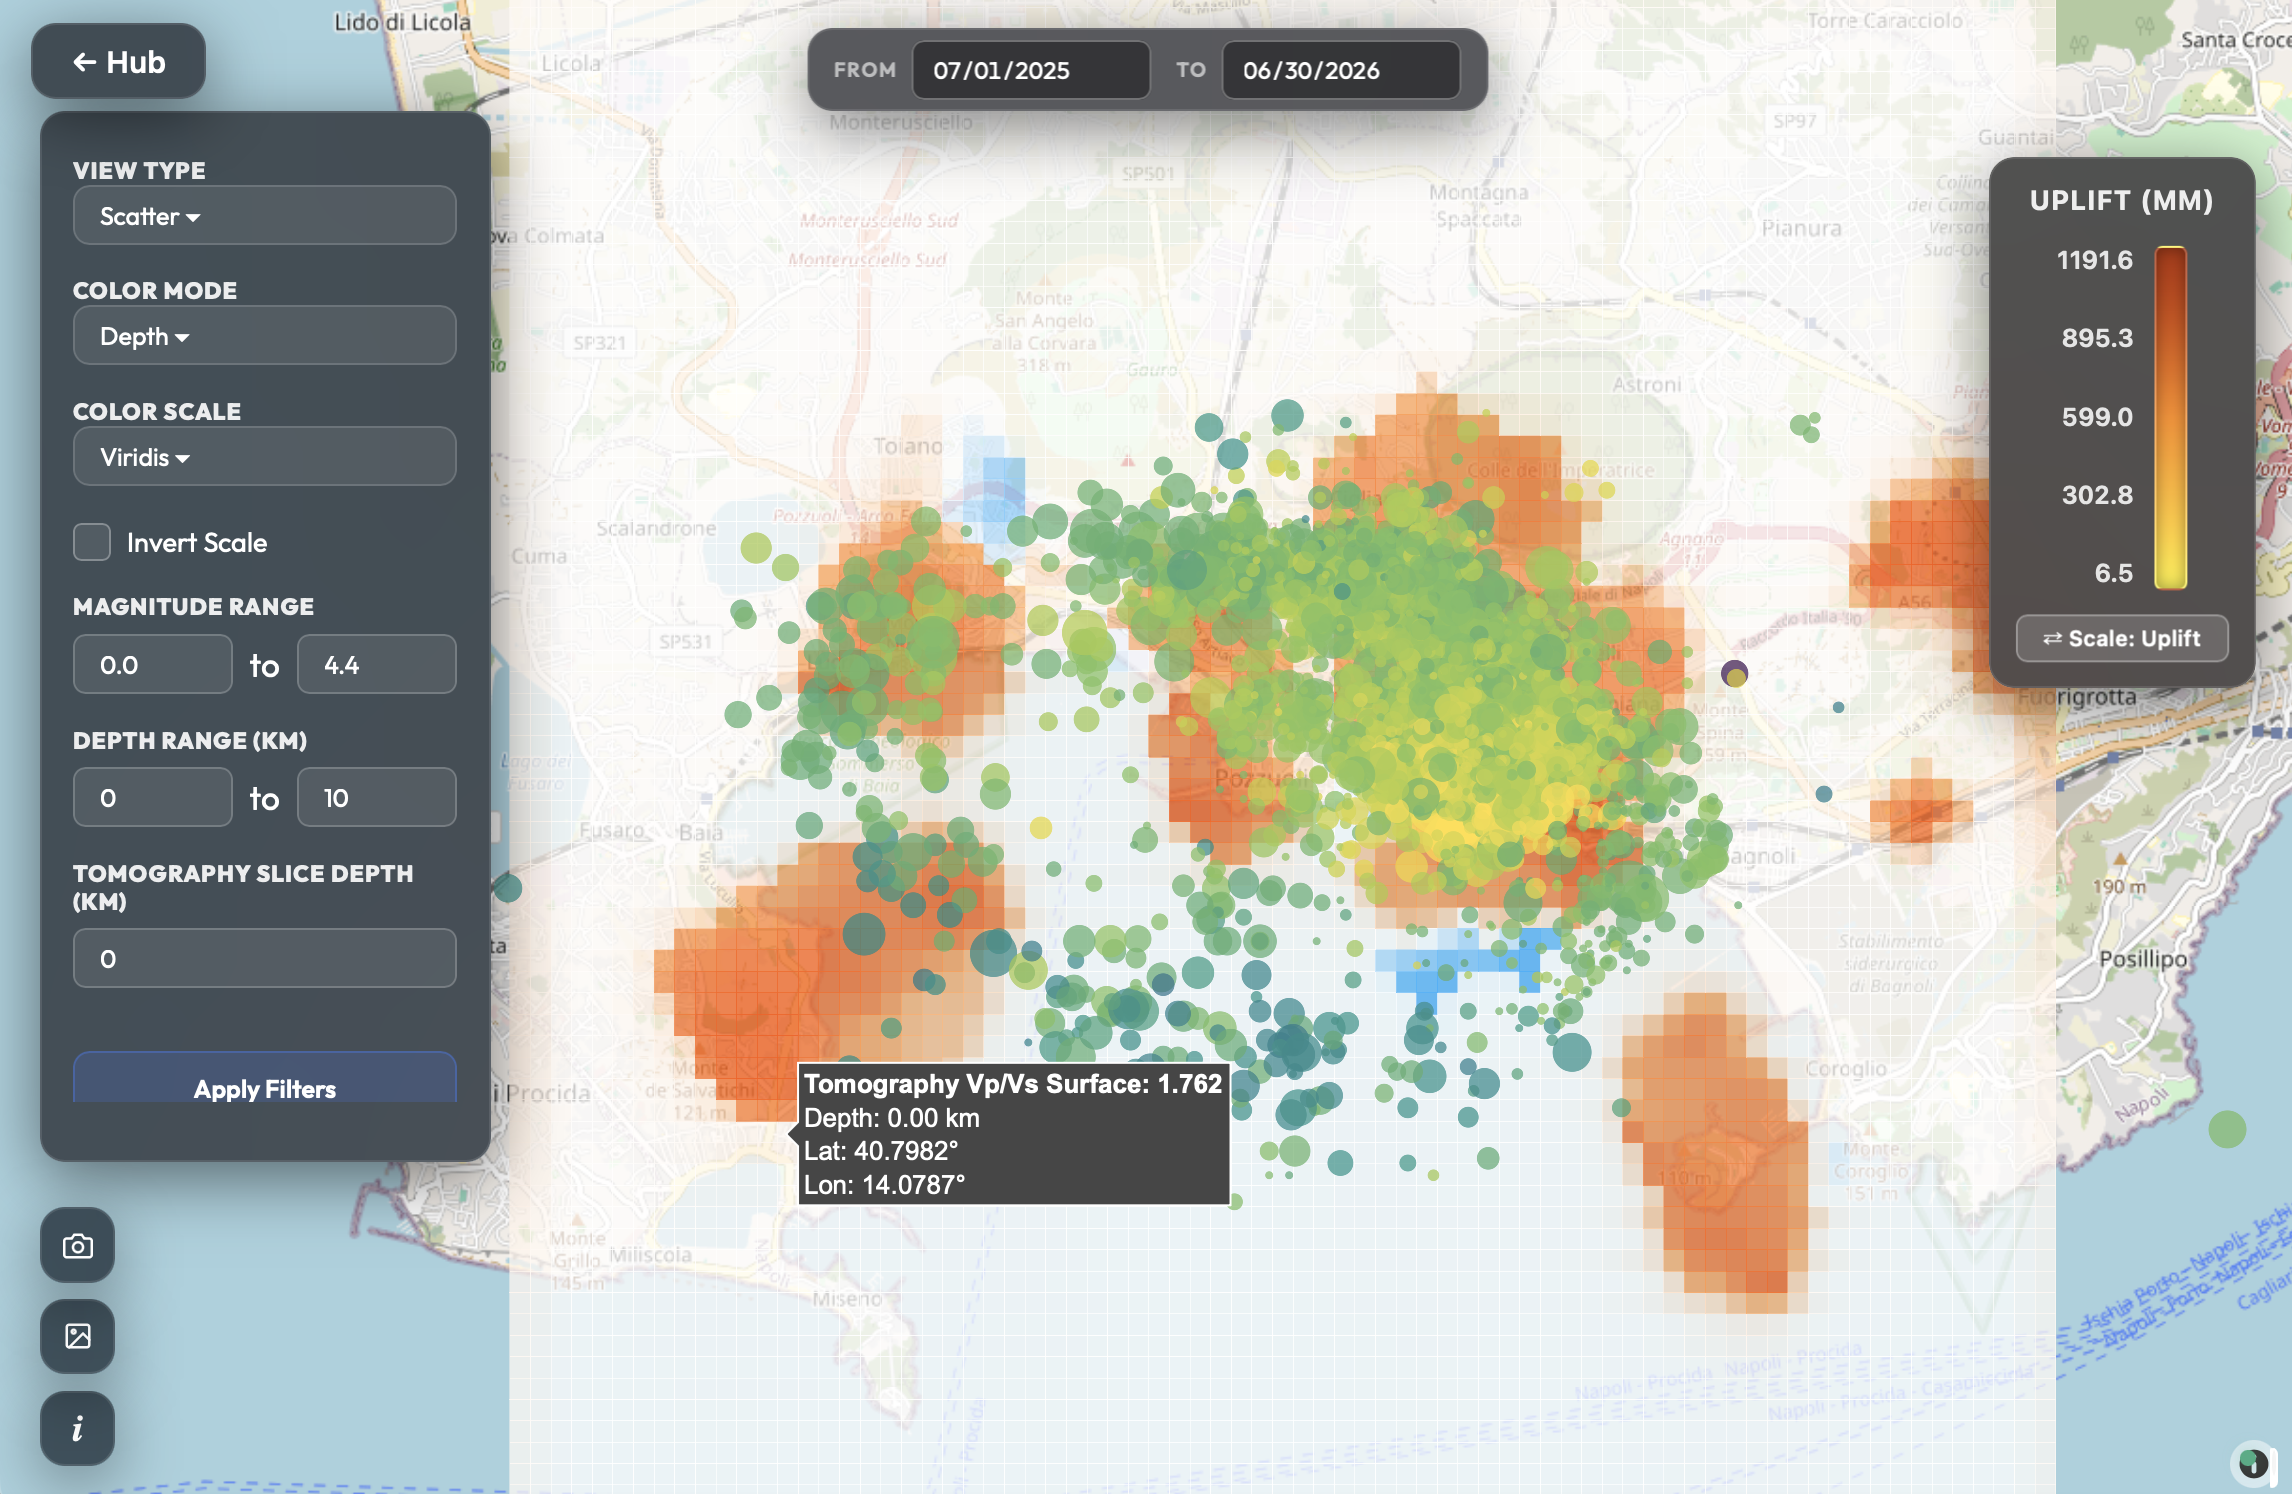
\includegraphics[width=\textwidth, height=0.66\textwidth]{images/2d_visualization_tomography.png}
\caption{An overlay showing a tomography slice of the crust. The highlighted areas indicate high $V_p/V_s$ velocity anomalies.}
\label{fig:2d-viz-tomo}
\end{subfigure}
\end{figure}

\begin{figure}[H]
\ContinuedFloat
\centering
\begin{subfigure}[t]{0.85\textwidth}
\centering
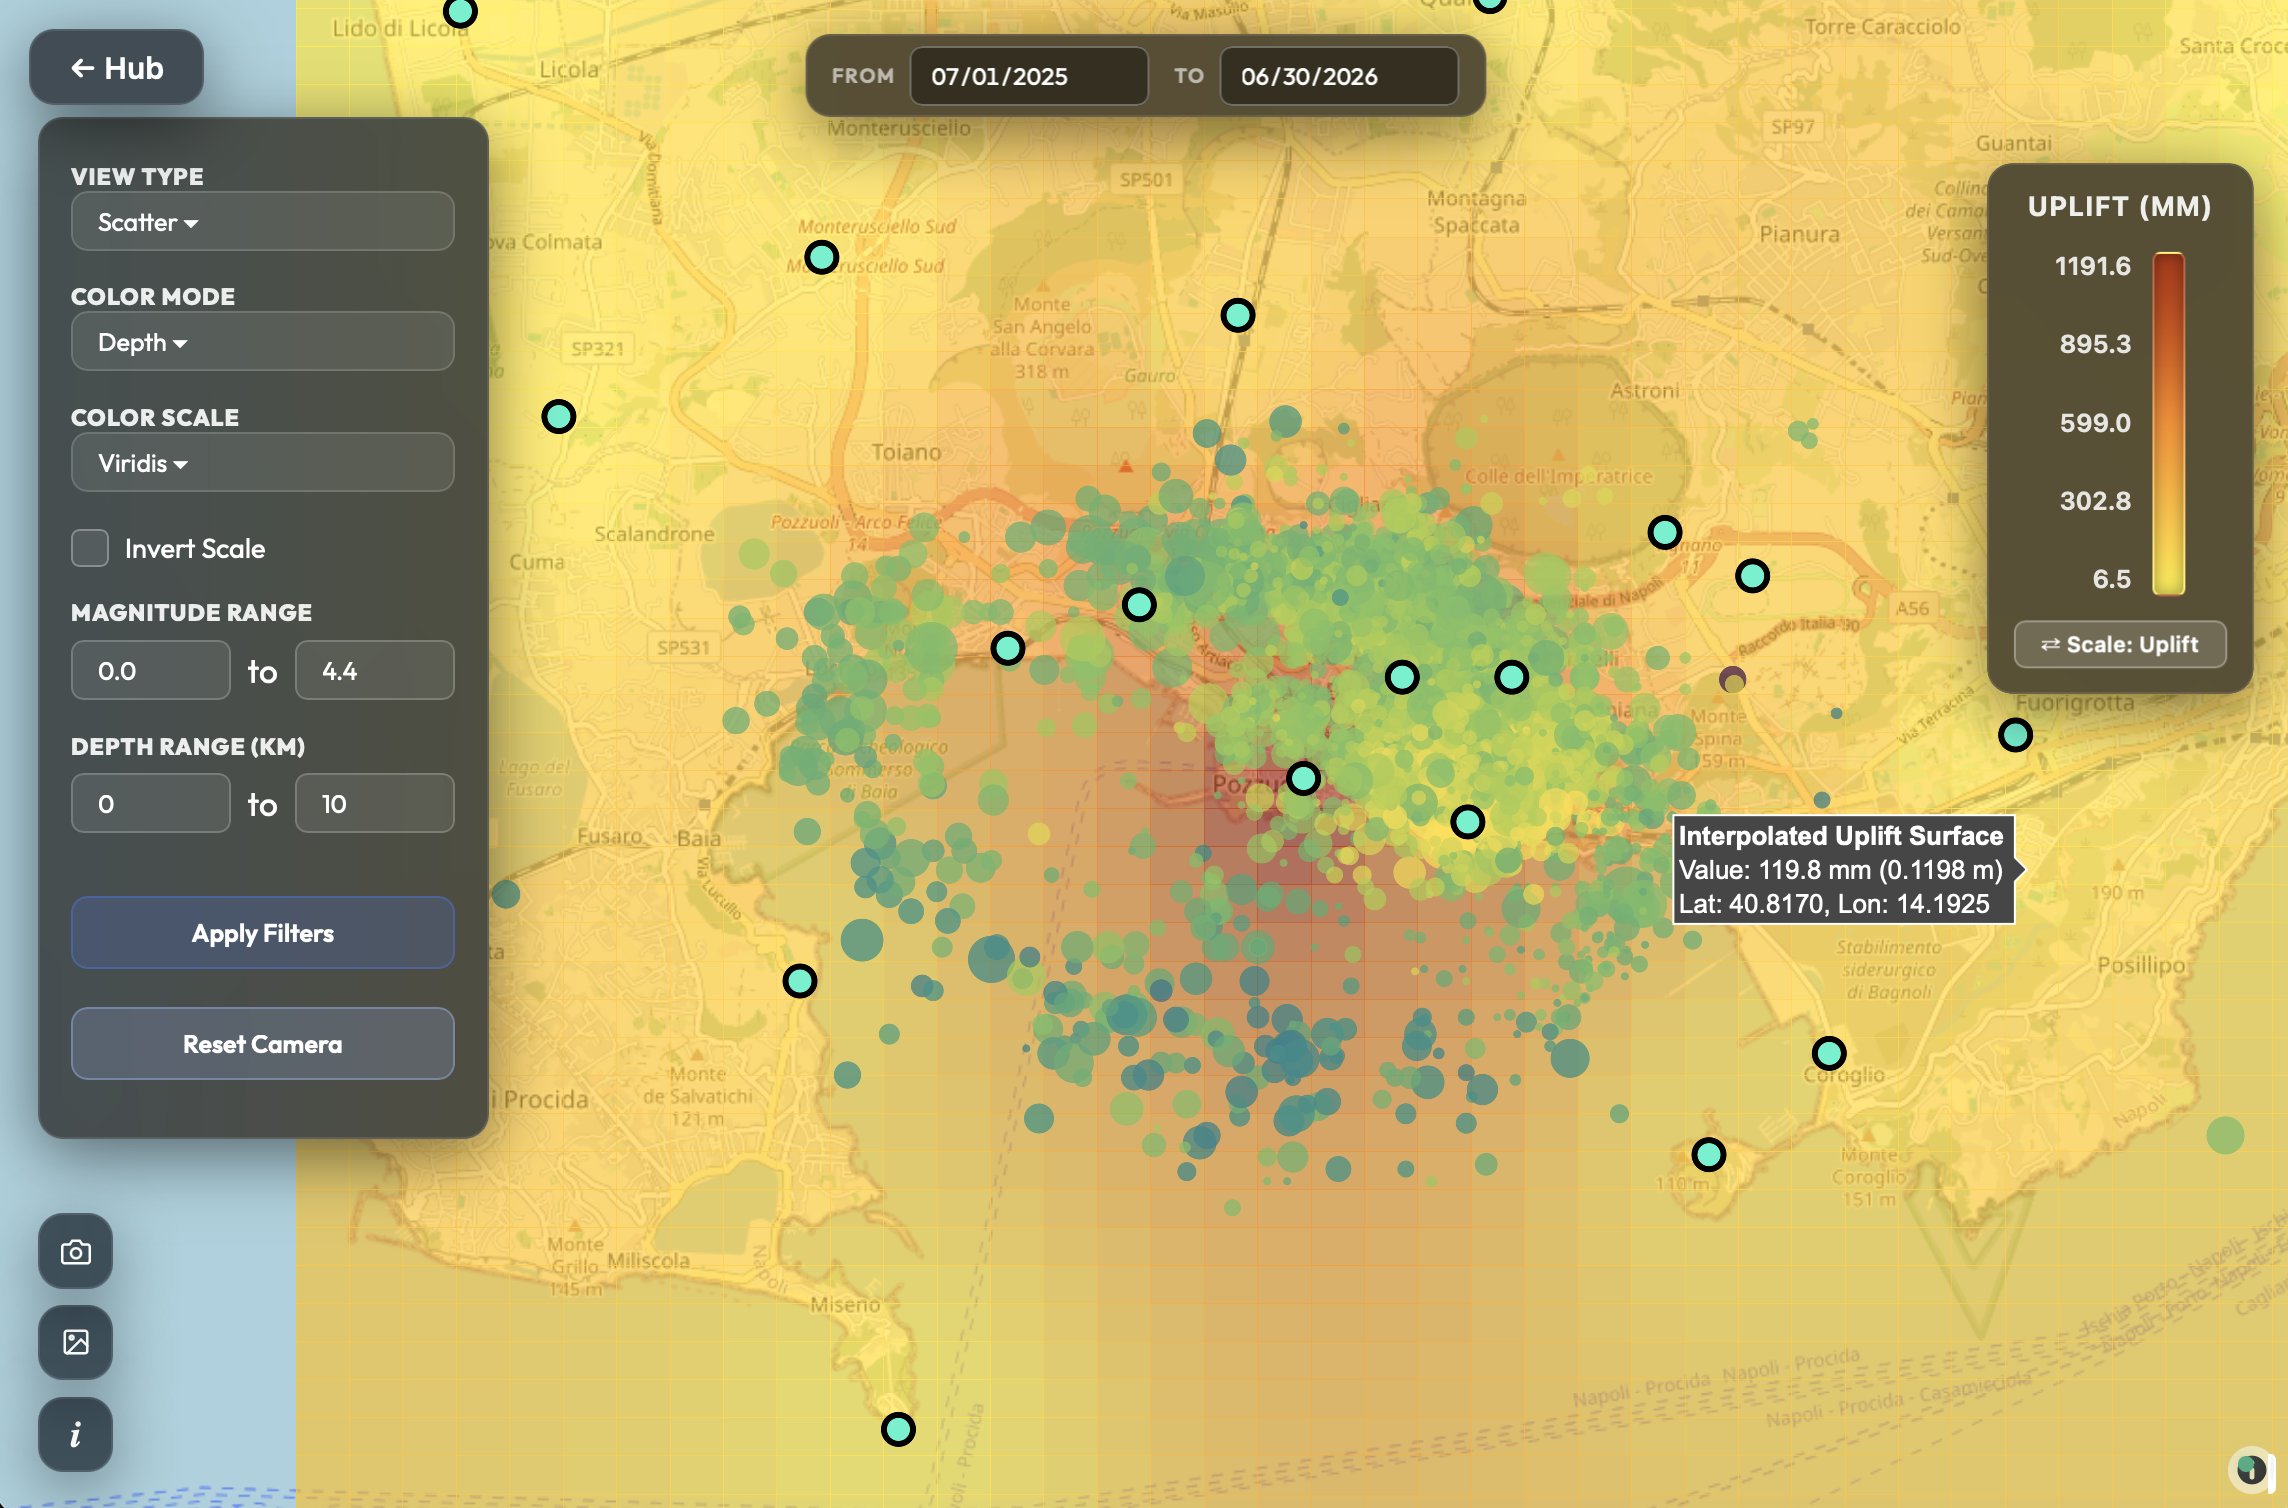
\includegraphics[width=\textwidth]{images/2d_visualization_uplift_stations.png}
\caption{An overlay displaying vertical ground movement (uplift) using a grid map, along with the locations of permanent monitoring stations across Campi Flegrei.}
\label{fig:2d-viz-uplift}
\end{subfigure}
\caption{The 2D Geospatial Map View in the Seismic Viewer. This workspace allows users to filter earthquake data (\subref{fig:2d-viz}) and combine it with advanced geophysical overlays, such as tomographic velocity maps (\subref{fig:2d-viz-tomo}) and ground uplift measurements (\subref{fig:2d-viz-uplift}).}
\label{fig:2d-multi}
\end{figure}

As shown in \Cref{fig:2d-multi}, the 2D workspace offers three visualisation options. The base view (\Cref{fig:2d-viz}) displays earthquake locations on an OpenStreetMap layer, while the side panel allows users to filter events by magnitude, depth, and date. In \Cref{fig:2d-viz-tomo}, a tomographic slice shows variations in the $V_p/V_s$ velocity ratio, indicating underground fluid bodies. Finally, in \Cref{fig:2d-viz-uplift}, the map combines monitoring stations with vertical ground movement, helping researchers observe if earthquakes match areas of surface uplift.

\section{3D Static View}
\label{sec:view-3d-static}

The 3D static view renders hypocentres as a subsurface point cloud within a three-dimensional geographic volume beneath an OpenStreetMap terrain surface. The reference terrain is rendered as a flat, unshaded map layer for clarity, while earthquakes are represented beneath the surface as a 3D point cloud, colour-coded by variables like depth or time.

To prevent geographic distortion caused by Earth's sphericity, the system scales horizontal proportions based on latitude:
\begin{equation}
    \text{ratio}_x = \frac{\Delta\lambda \cdot K \cdot \cos(\bar{\phi})}{\max(d_\text{lon}, d_\text{lat})}, \quad
    \text{ratio}_y = \frac{\Delta\phi \cdot K}{\max(d_\text{lon}, d_\text{lat})}
    \label{eq:aspect-ratio}
\end{equation}
where $\Delta\lambda$ and $\Delta\phi$ are the longitude and latitude spans, $K = 111.32$~km/° is the equatorial conversion factor, and $\bar{\phi}$ is the mean latitude. This adjustment preserves accurate spatial proportions.

Rendering large point clouds simultaneously relies on GPU acceleration. Plotly.js uses WebGL to draw points via the \texttt{scatter3d} trace type. To maintain smooth interactive frame rates, the application applies three measures: (1) map background images are scaled to save memory, (2) automatic bounding box recalculations are disabled during updates, and (3) markers are drawn as point sprites facing the camera rather than complex 3D shapes.

As shown in \Cref{fig:3d-multi}, the 3D static workspace presents these data layers in three dimensions. The base view (\Cref{fig:3d-viz}) shows hypocentres below the map surface, using colours to represent depth intervals. In \Cref{fig:3d-viz-tomo}, the scene adds velocity slices from the tomography model. Finally, in \Cref{fig:3d-viz-uplift}, vertical columns indicate surface movement at each station, allowing direct comparisons between depth and surface observations.

\begin{figure}[H]
\centering
\begin{subfigure}[t]{1.0\textwidth}
\centering
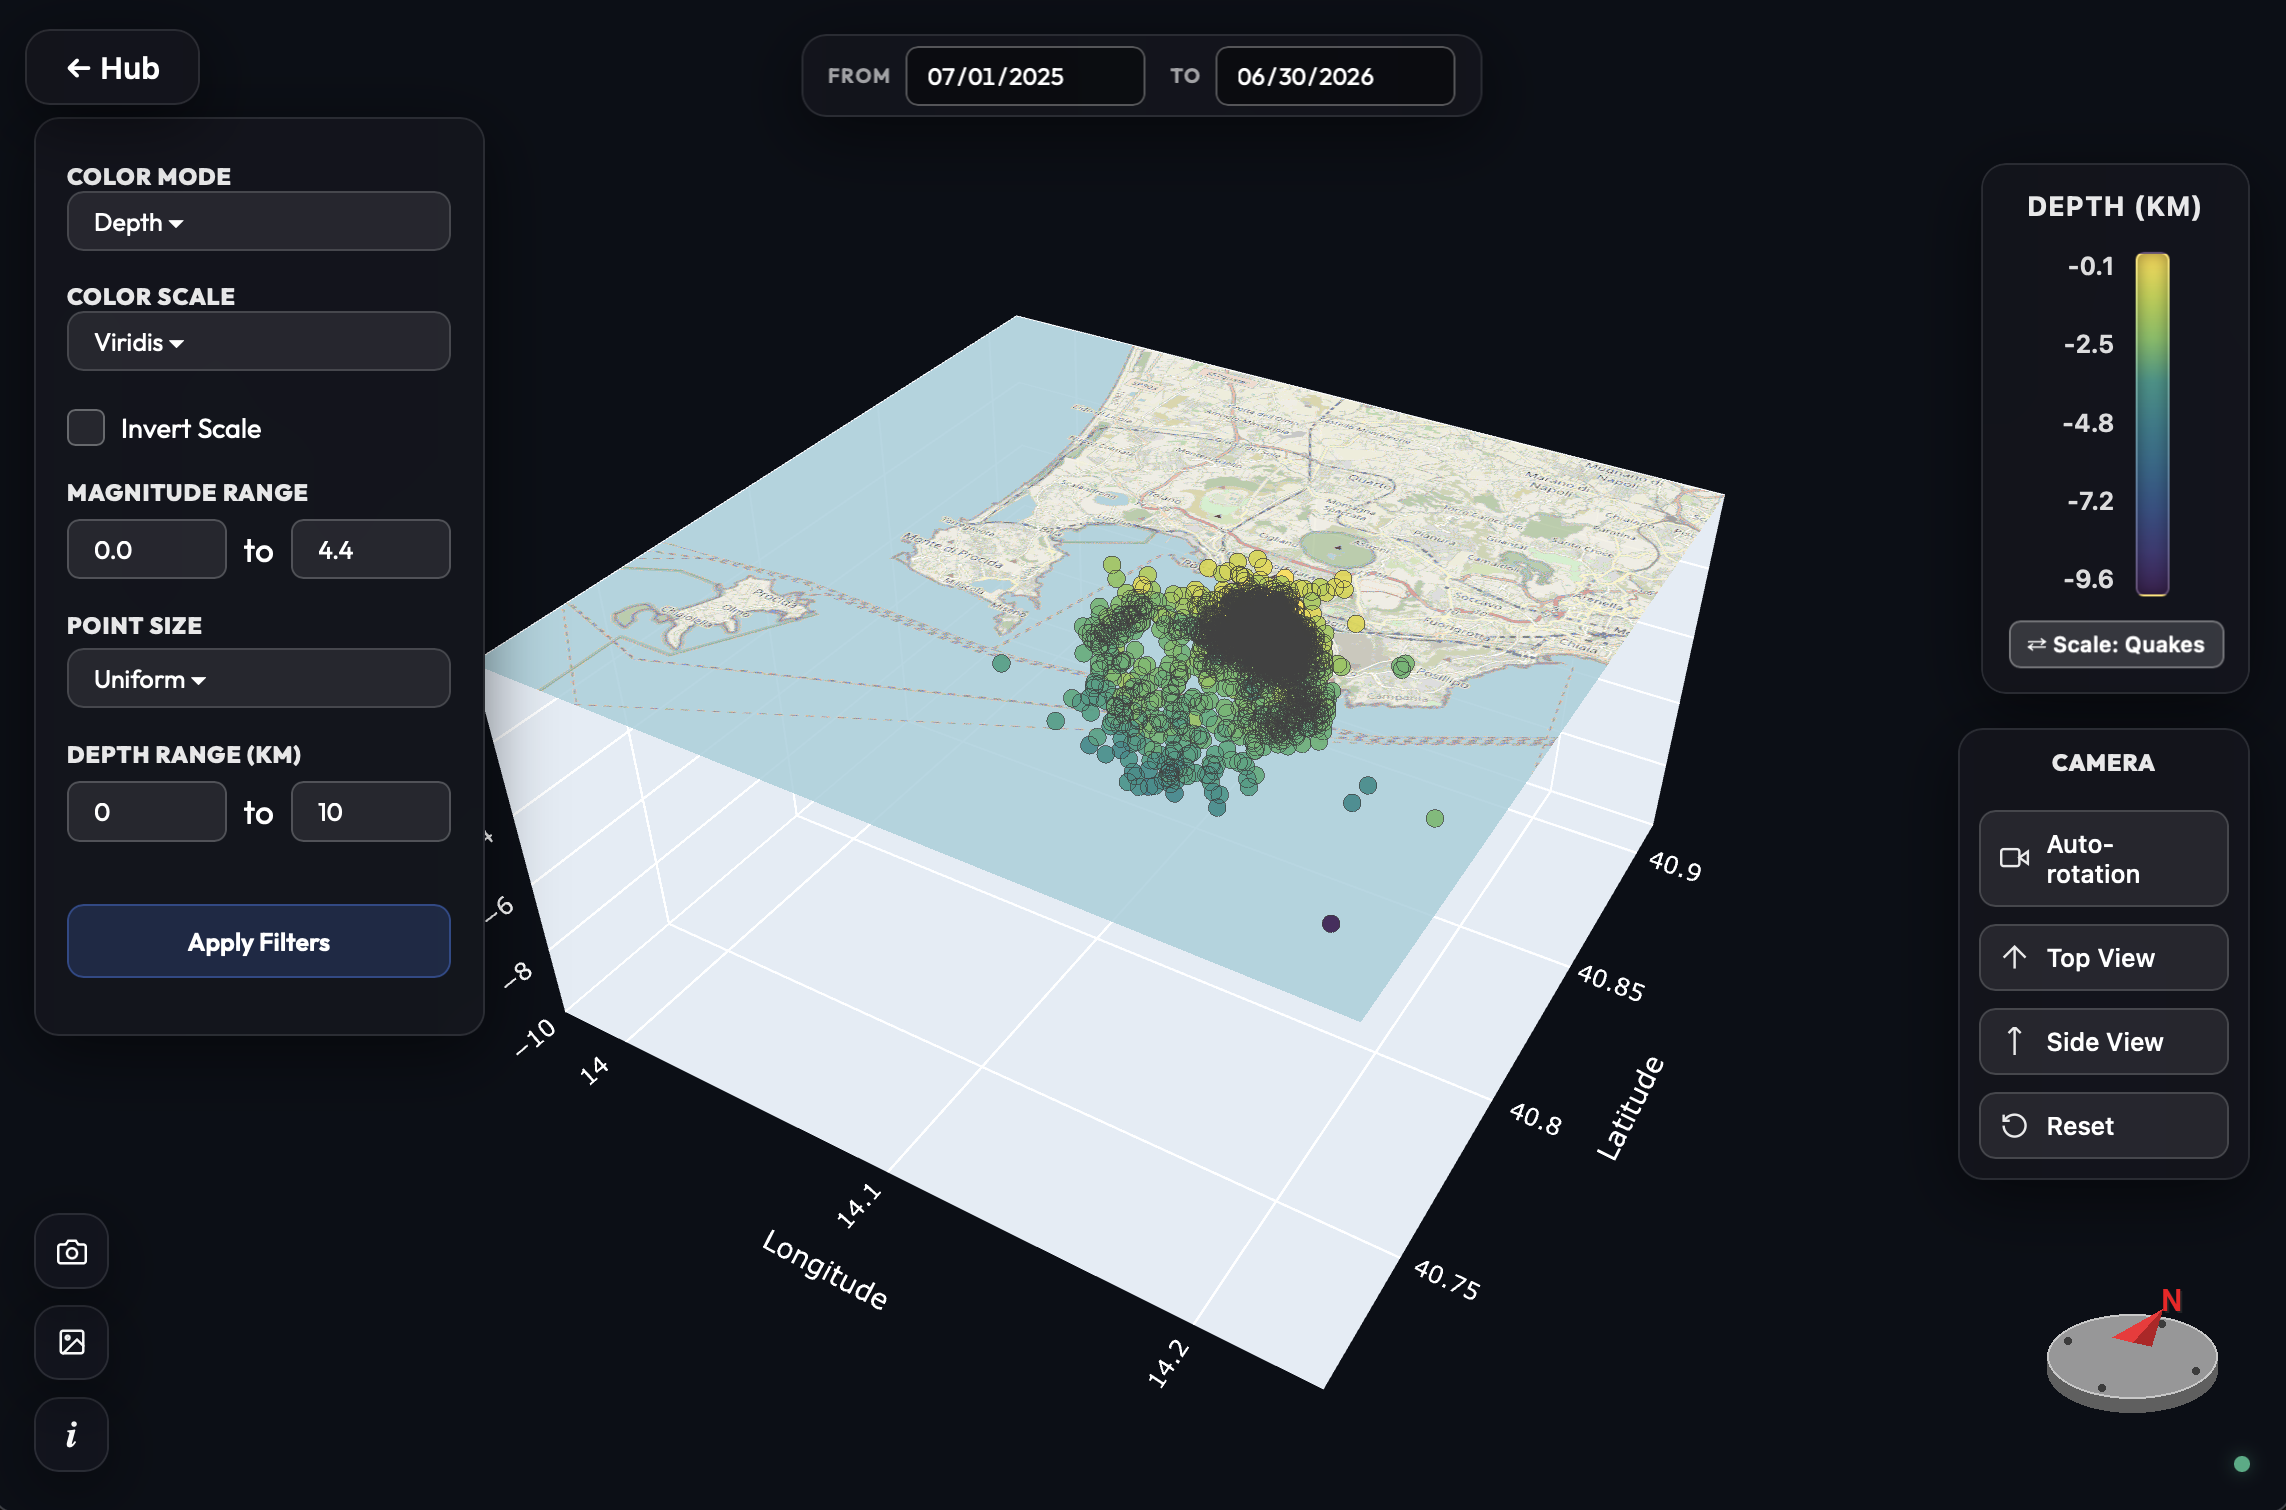
\includegraphics[width=\textwidth]{images/3d_visualization.png}
\caption{Point cloud below surface map.}
\label{fig:3d-viz}
\end{subfigure}
\end{figure}

\begin{figure}[H]
\ContinuedFloat
\centering
\begin{subfigure}[t]{1.0\textwidth}
\centering
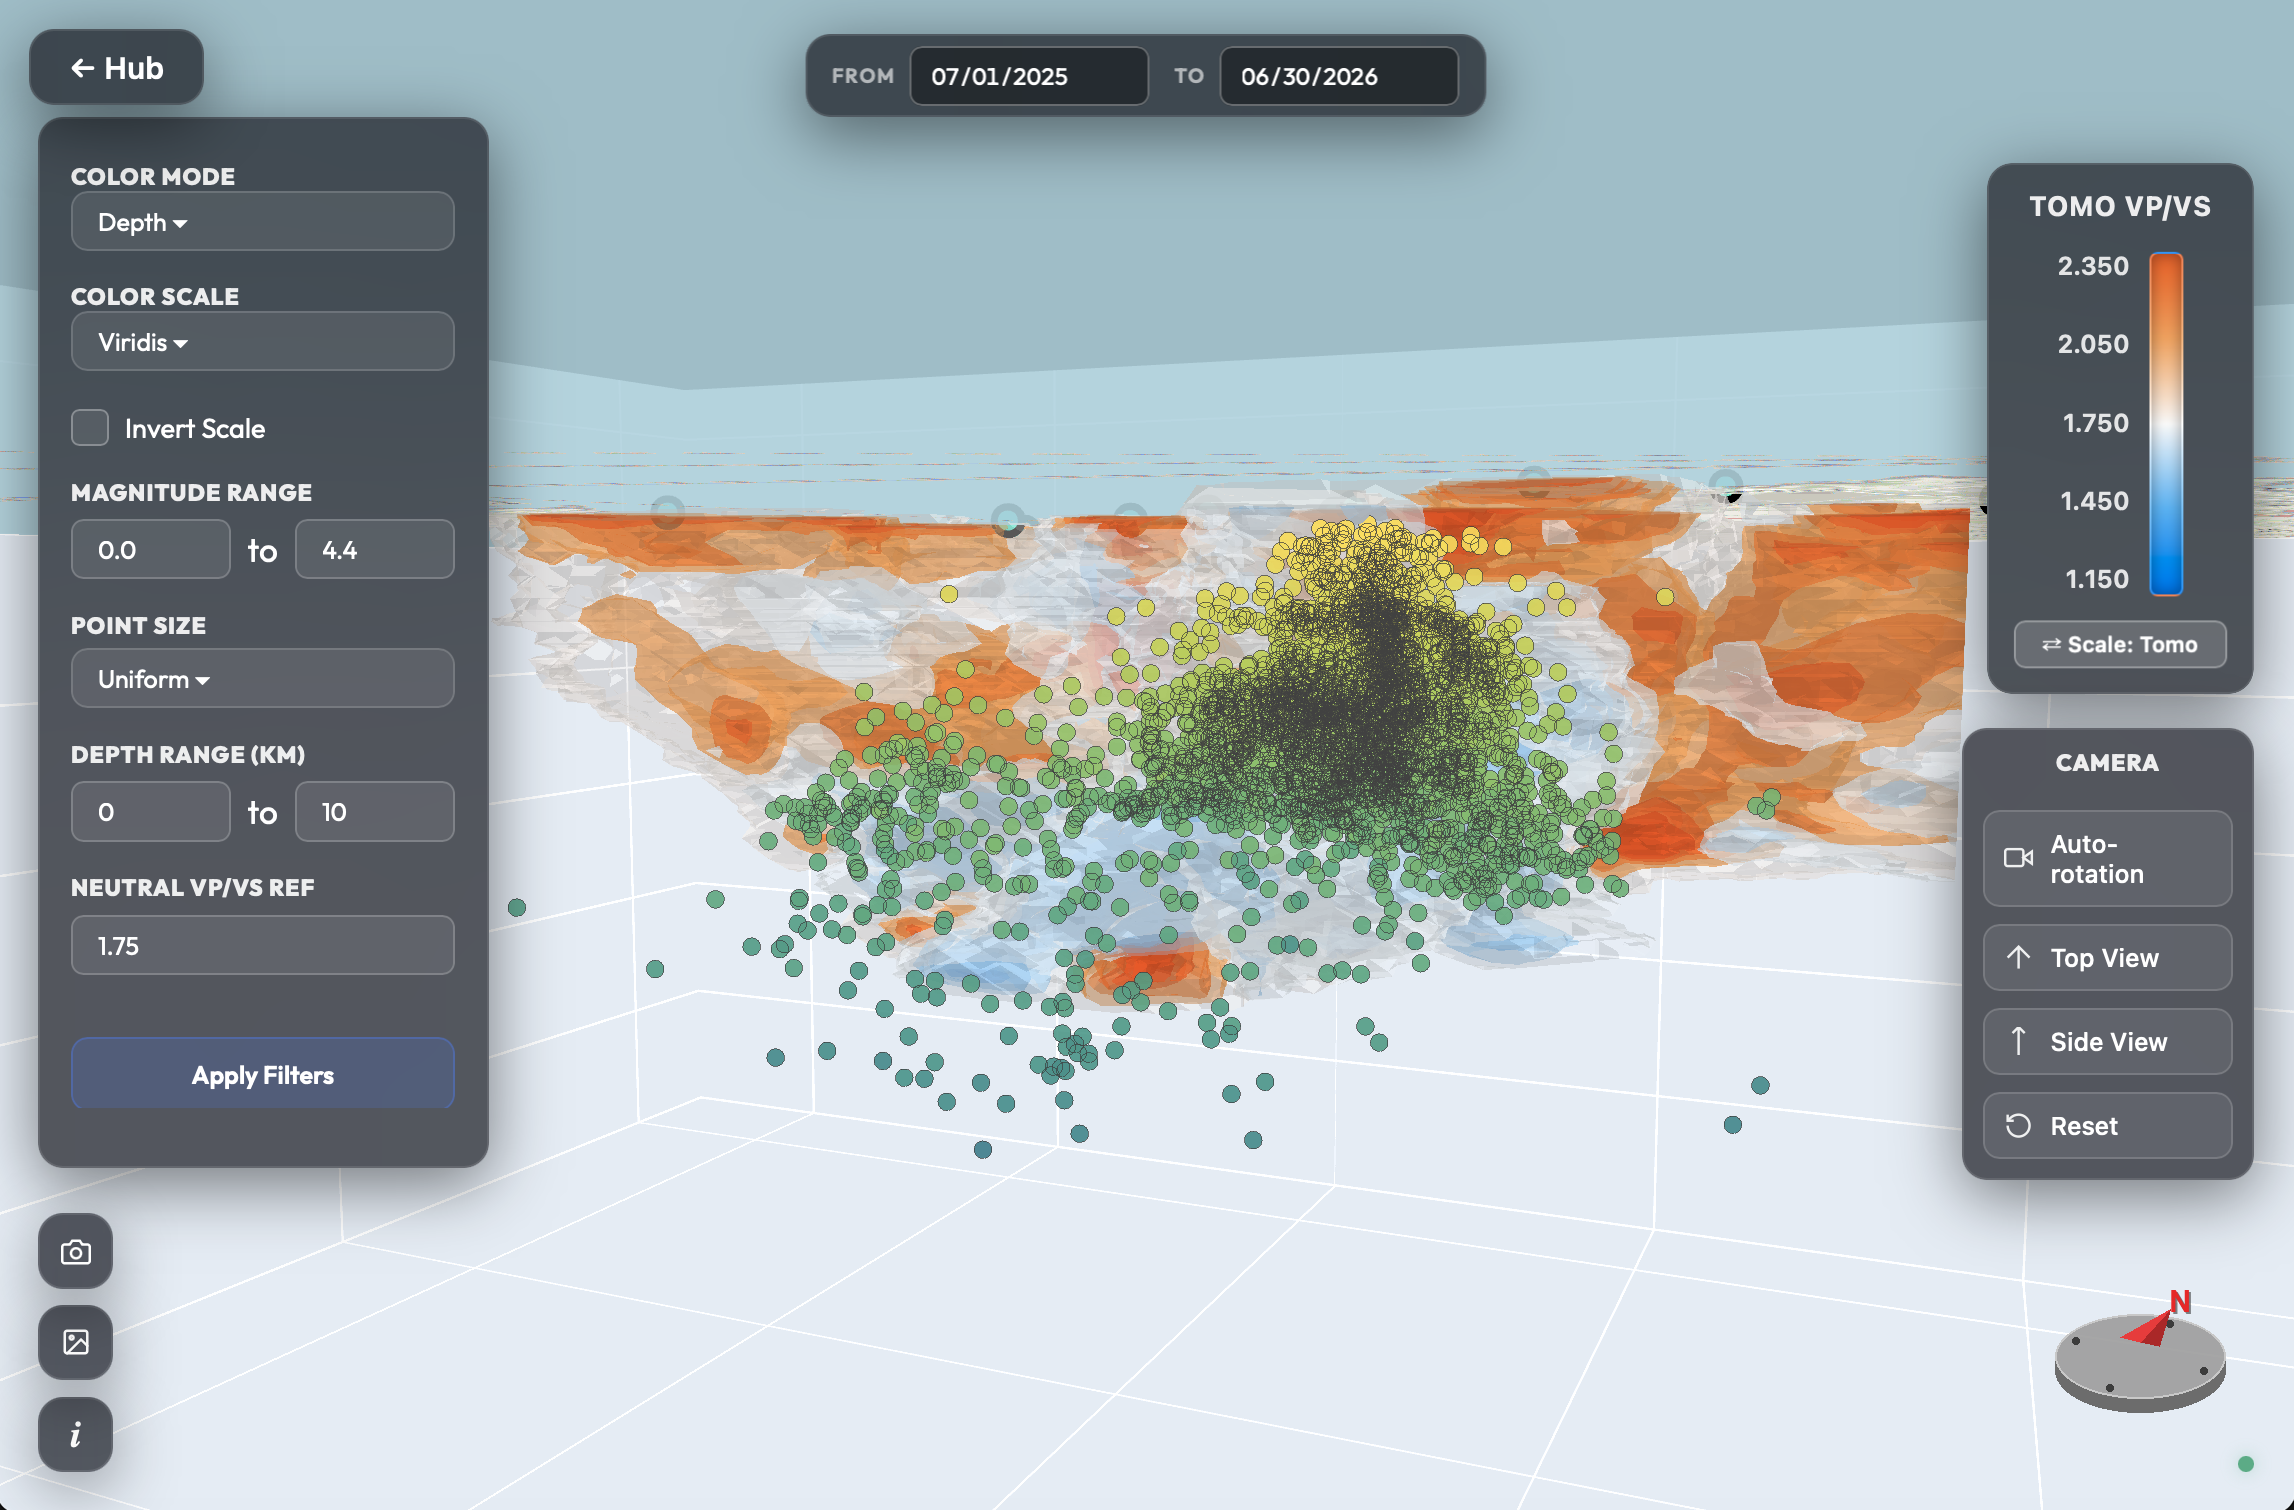
\includegraphics[width=\textwidth]{images/3d_visualization_tomography.png}
\caption{Added tomography layer.}
\label{fig:3d-viz-tomo}
\end{subfigure}
\end{figure}

\begin{figure}[H]
\ContinuedFloat
\centering
\begin{subfigure}[t]{1.0\textwidth}
\centering
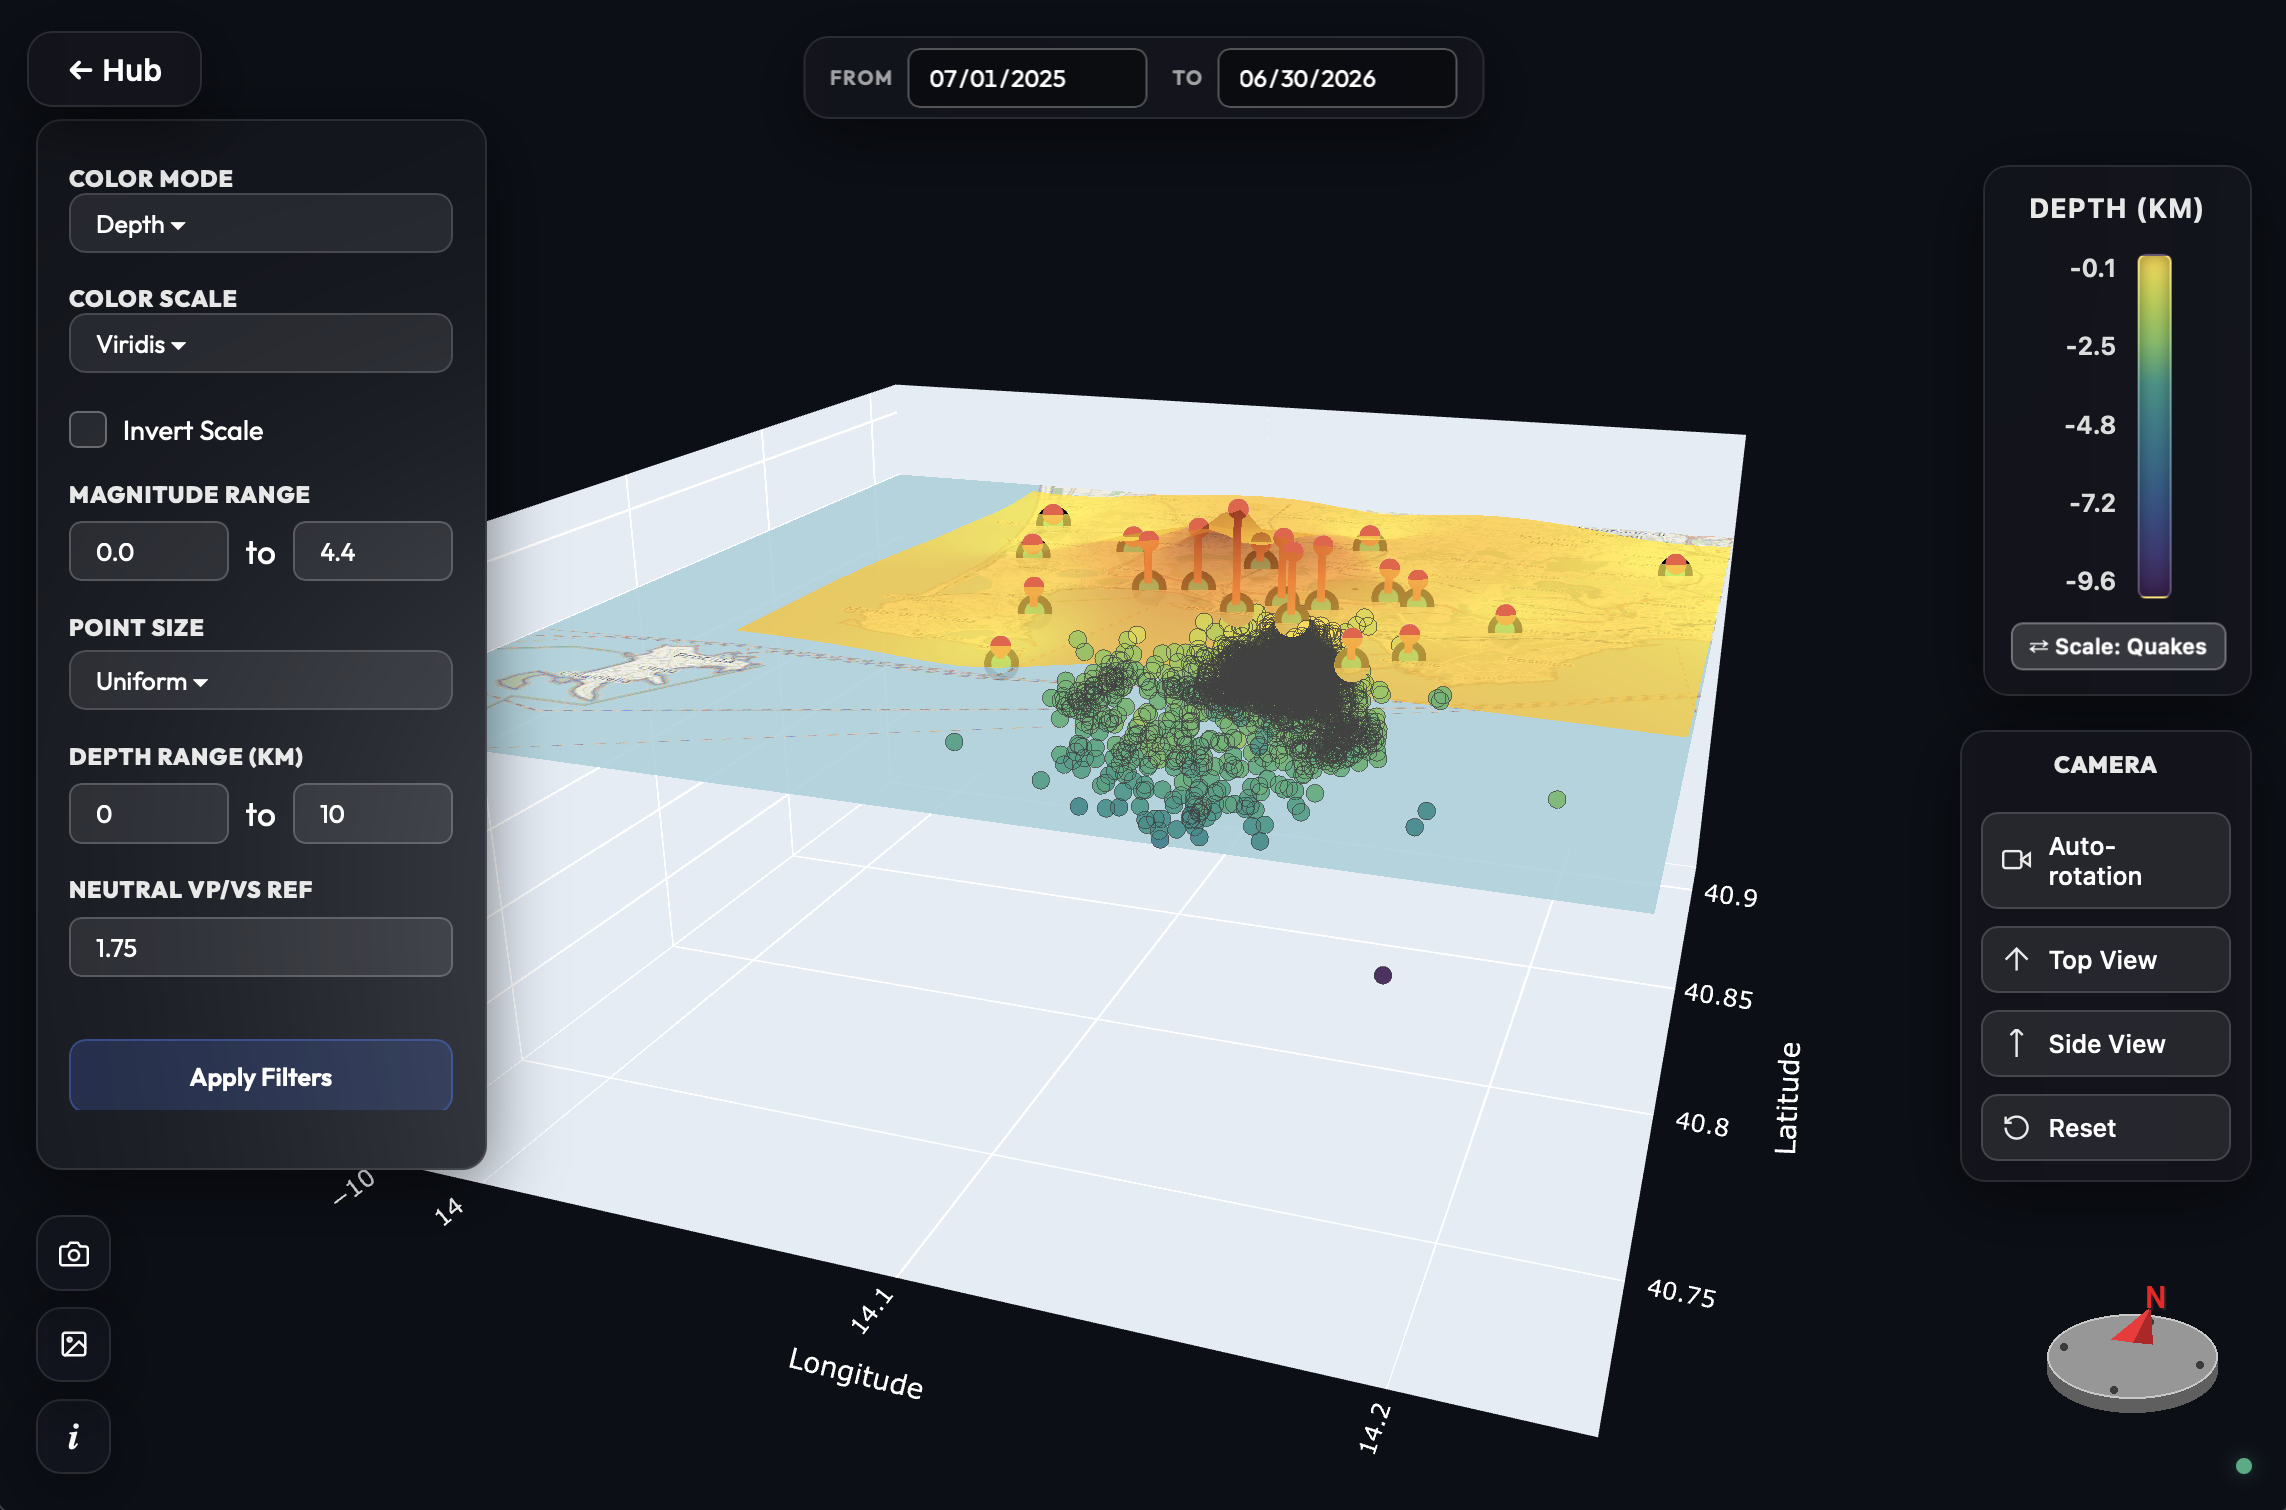
\includegraphics[width=\textwidth]{images/3d_visualization_uplift_stations.png}
\caption{Ground uplift columns.}
\label{fig:3d-viz-uplift}
\end{subfigure}
\caption{The 3D Static View workspace. The user can explore the underground earthquake distribution (\subref{fig:3d-viz}) and combine it with 3D tomography models (\subref{fig:3d-viz-tomo}) and surface deformation data (\subref{fig:3d-viz-uplift}).}
\label{fig:3d-multi}
\end{figure}

\section{3D Animated View (4D Visualisation)}
\label{sec:view-animated}

The animated view adds time as a fourth dimension to observe the spatio-temporal evolution of seismic sequences.

The 4D visualisation engine offers four temporal modes to analyse seismic evolution: \textbf{Accumulation} (showing all events up to the current frame), \textbf{Sliding window} (displaying events within a moving time frame), \textbf{Block mode} (rendering discrete, non-overlapping time intervals), and \textbf{Seismic Swarms} (focusing on episodic bursts identified by automated detection according to INGV criteria, supported by timeline navigation and magnitude or depth charts). To ensure smooth playback and avoid memory overload, the system precomputes temporal indices and updates the 3D scene dynamically without reloading the entire figure.

During 4D animations, the camera angle and zoom level must remain stable across updates. By default, Plotly reinitialises the view on coordinate changes. Setting \texttt{uirevision='constant'} in the layout preserves camera position and orientation across frames, allowing continuous interaction during playback.

\enlargethispage{5cm}

\begin{figure}[H]
\centering
\begin{subfigure}[t]{0.85\textwidth}
\centering
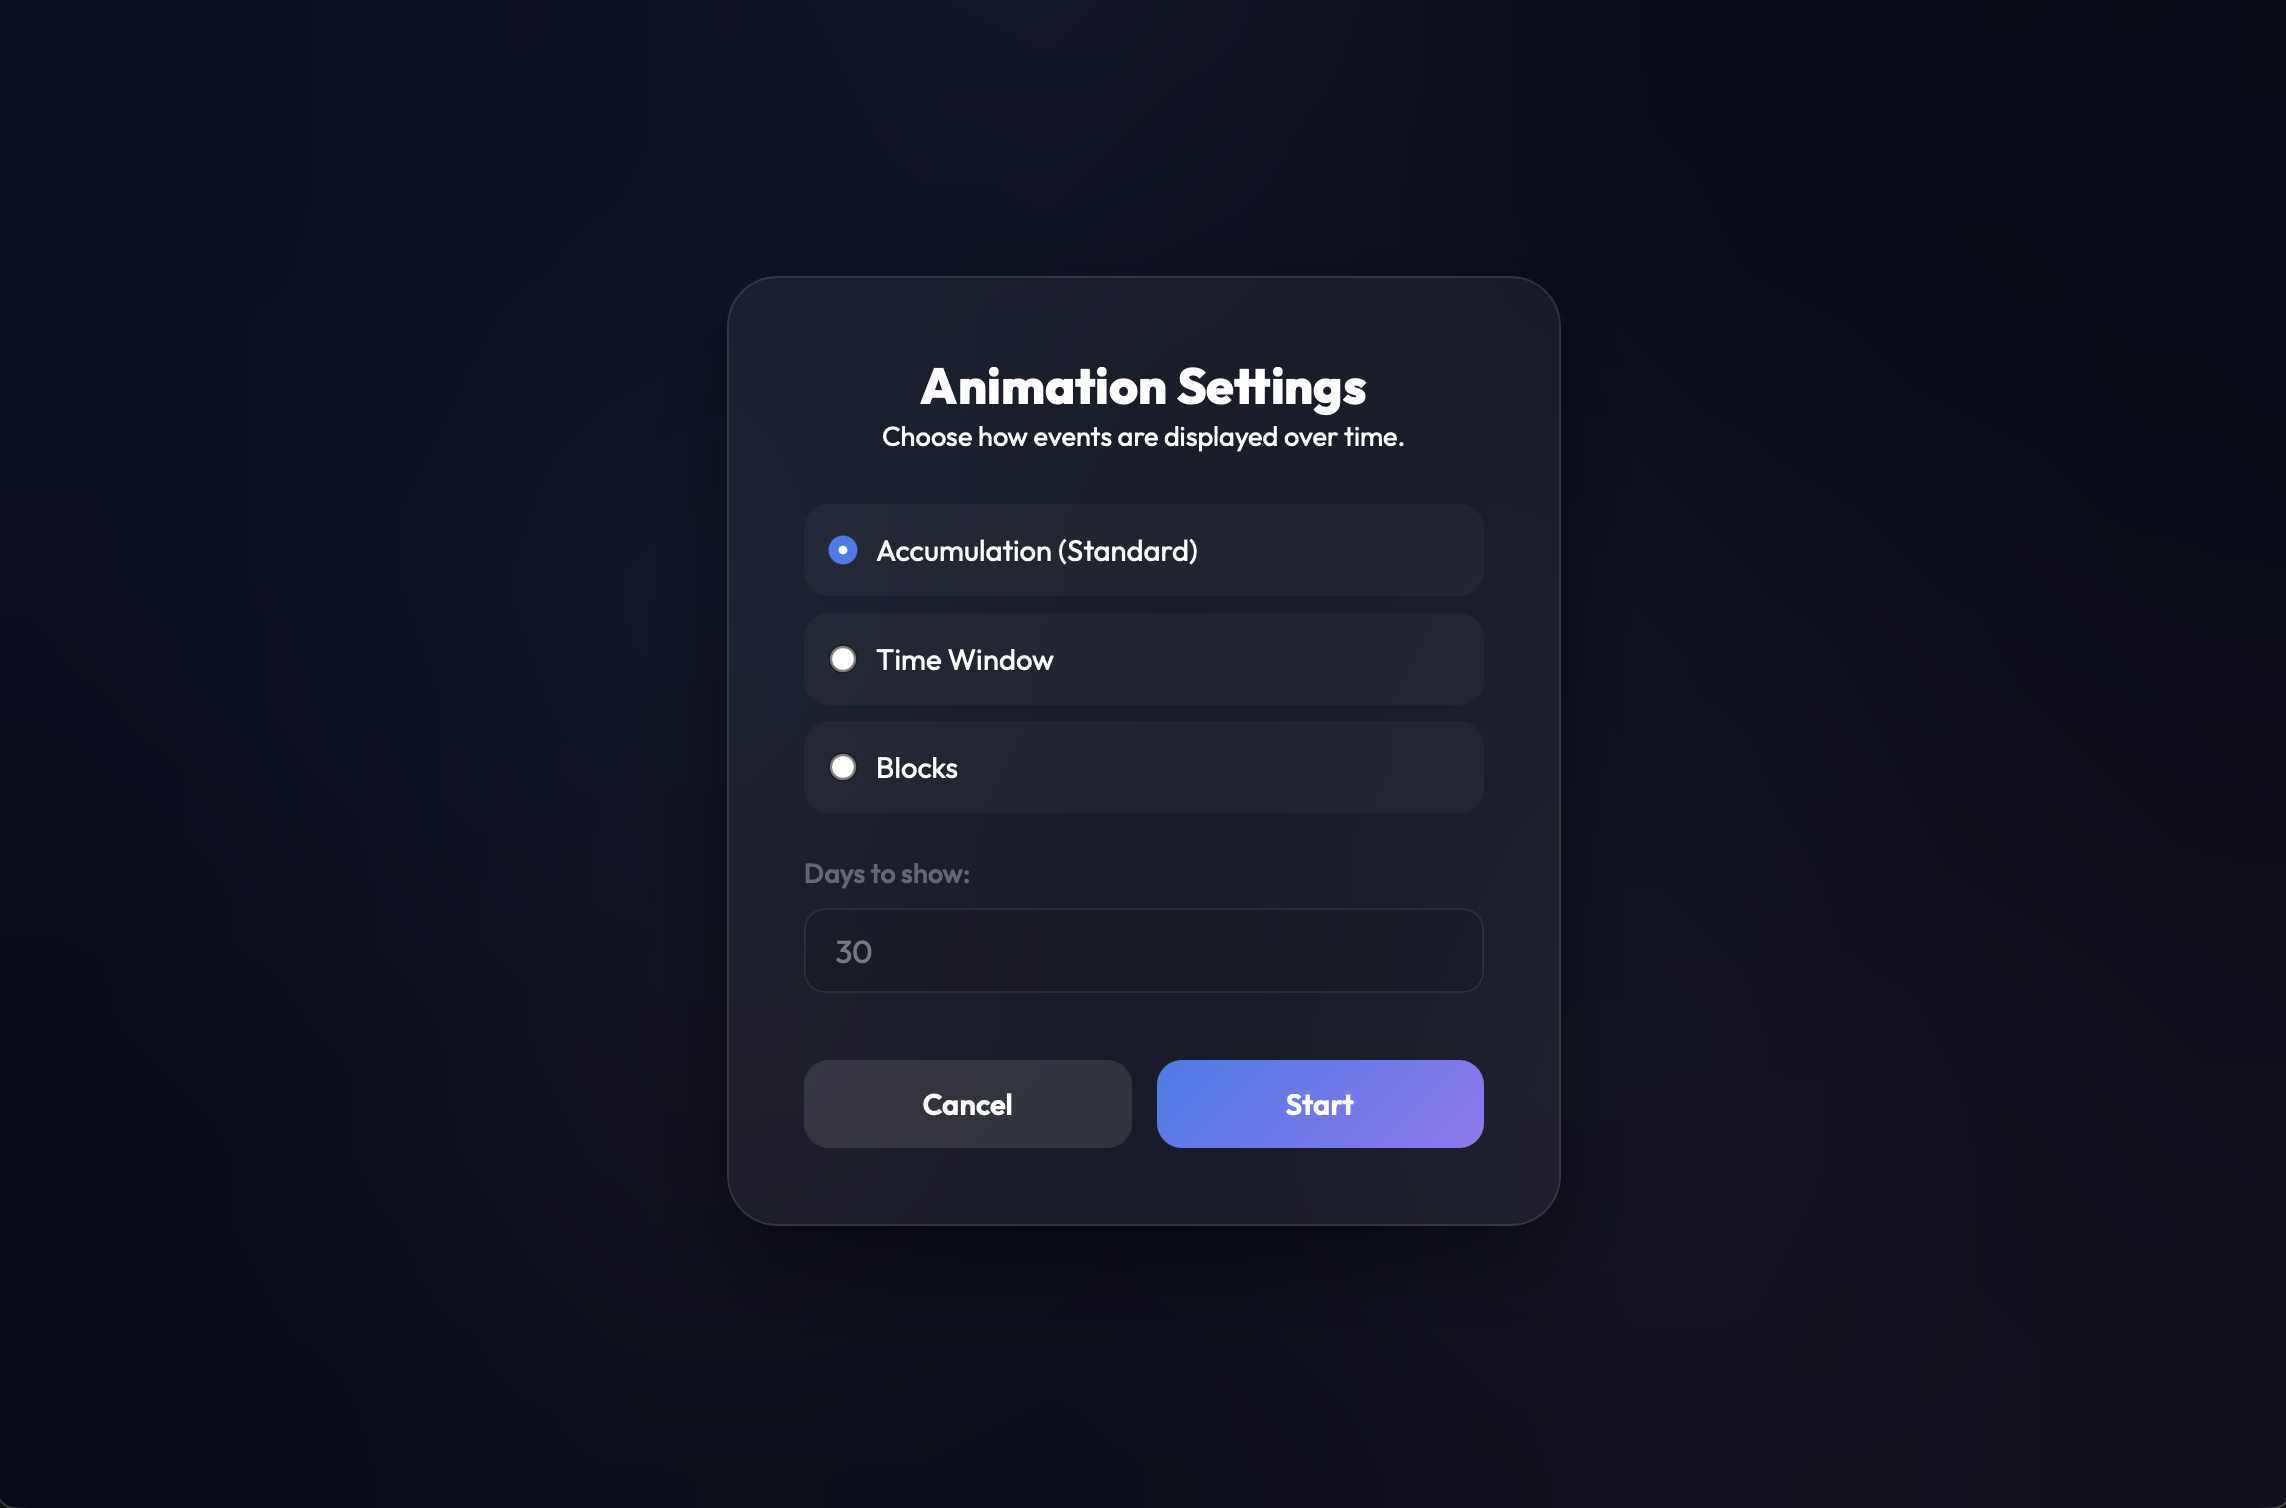
\includegraphics[width=\textwidth]{images/animated_visualization_selection_menu.png}
\caption{Temporal window configuration dialog.}
\label{fig:anim-menu}
\end{subfigure}
\end{figure}

\begin{figure}[H]
\ContinuedFloat
\centering
\begin{subfigure}[t]{0.85\textwidth}
\centering
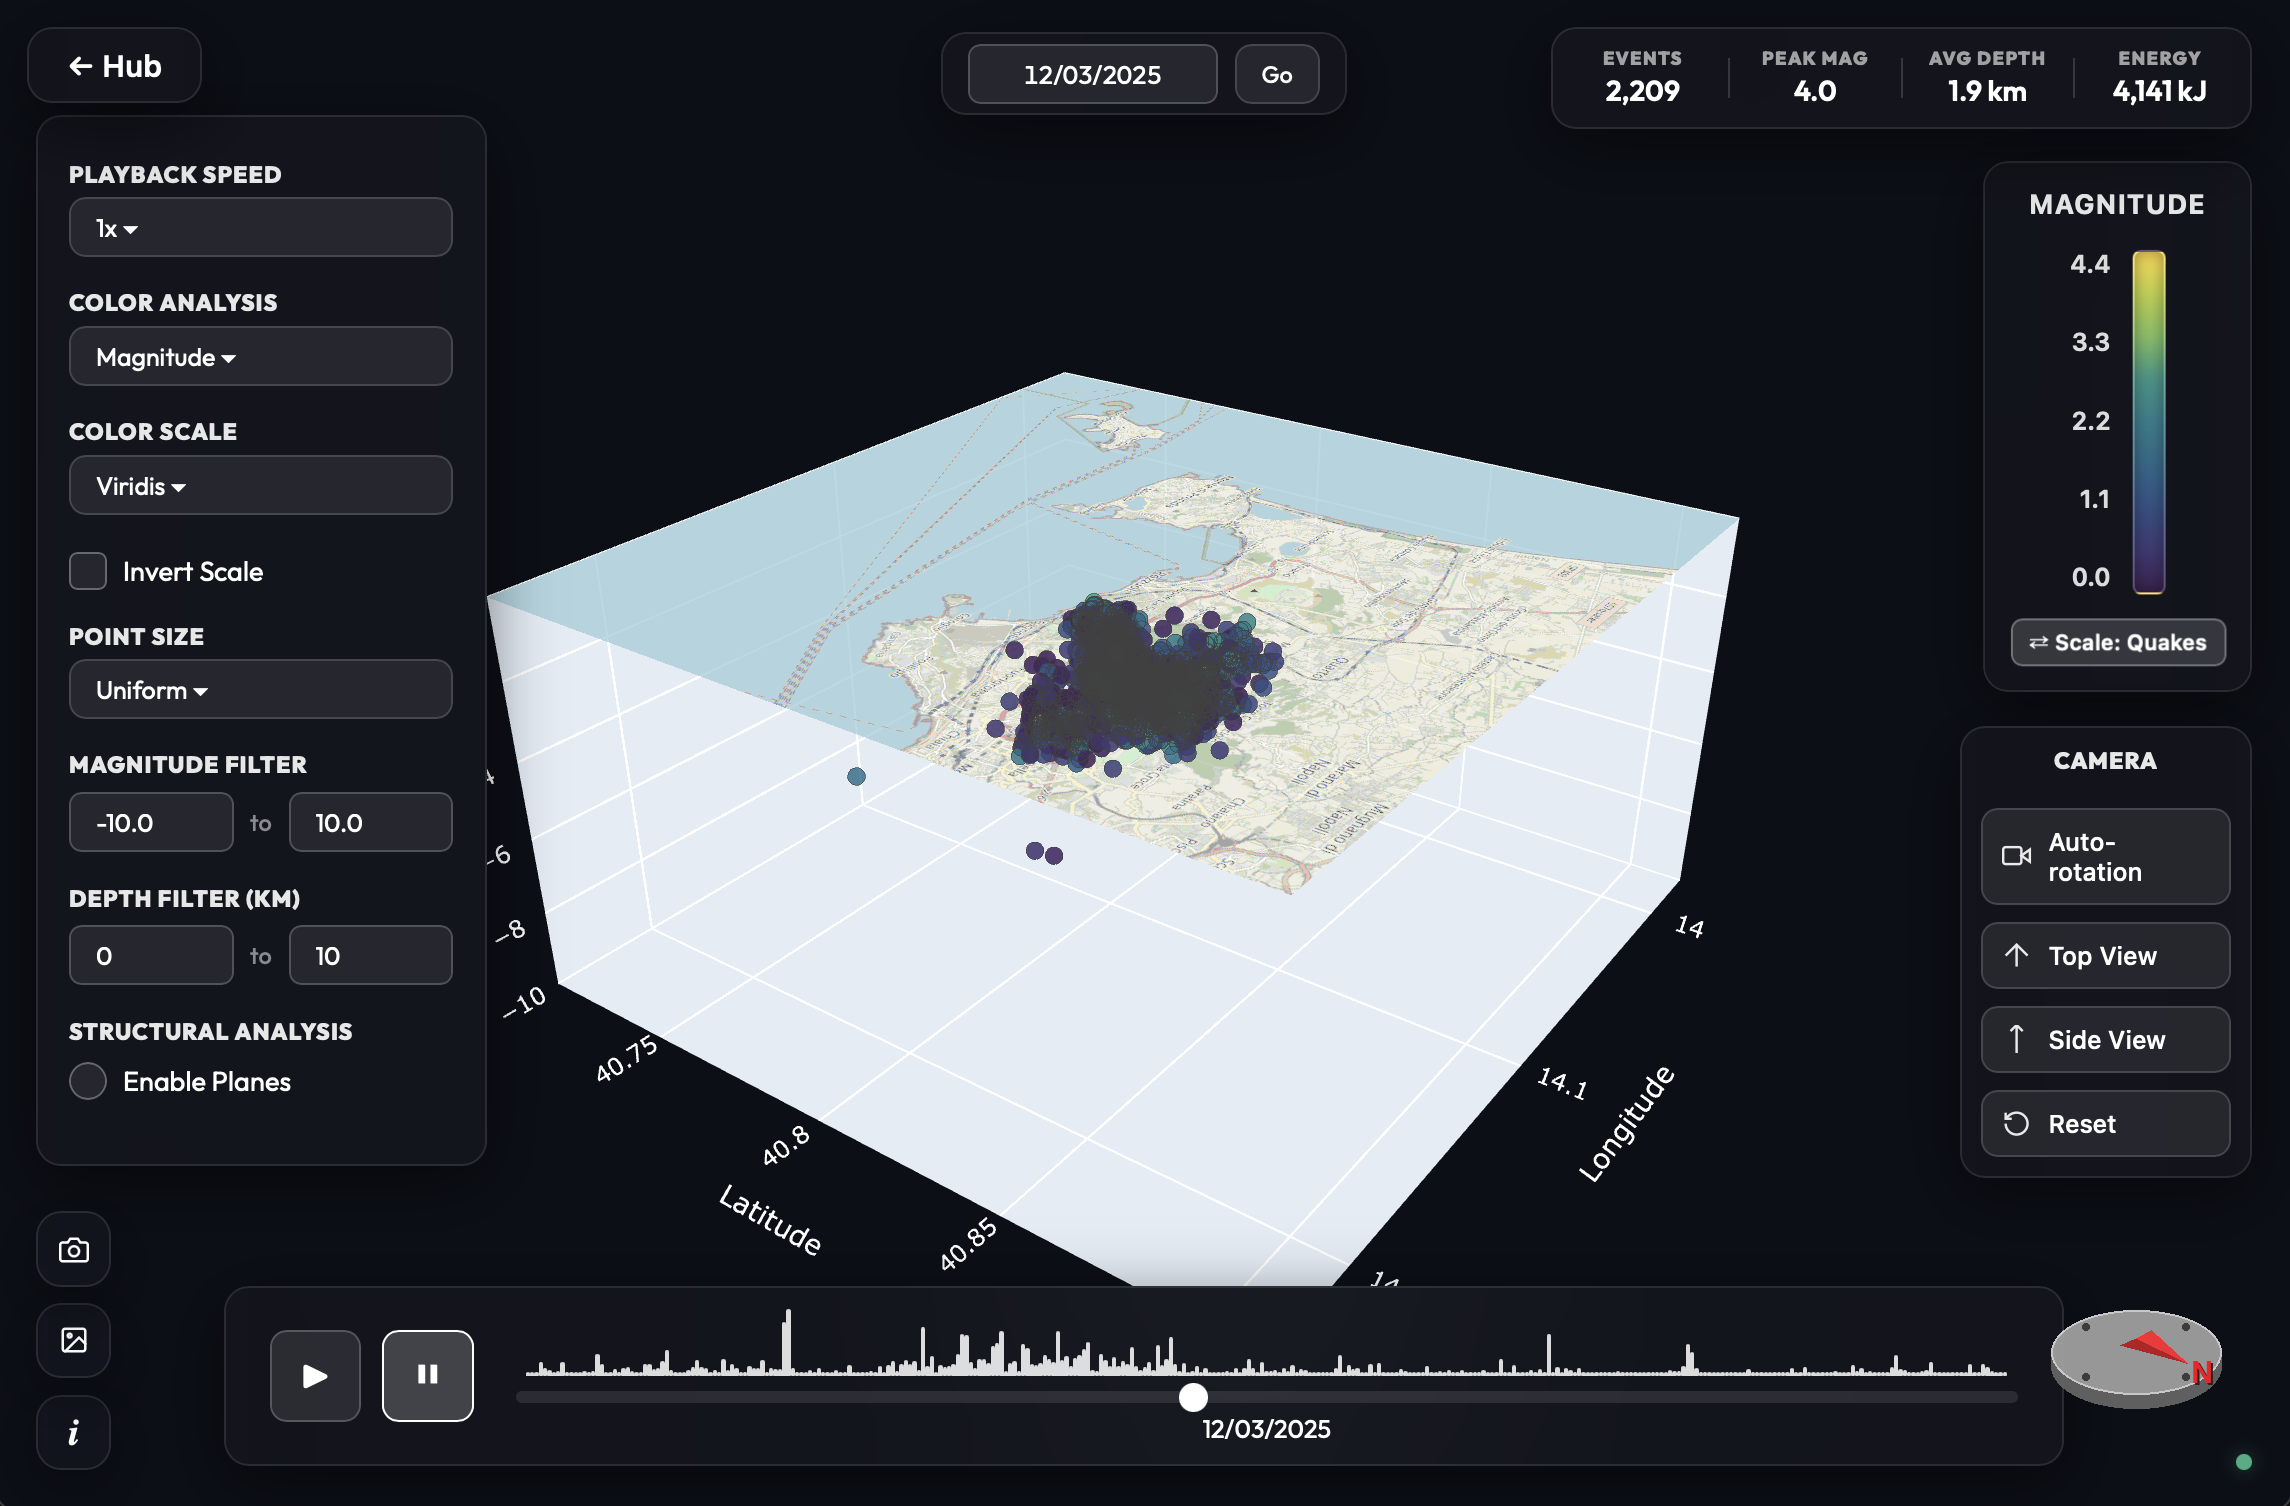
\includegraphics[width=\textwidth]{images/animated_visualization.png}
\caption{Active 4D playback view showing the time-sliced hypocentral point cloud.}
\label{fig:anim-viz}
\end{subfigure}
\end{figure}

\begin{figure}[H]
\ContinuedFloat
\centering
\begin{subfigure}[t]{0.85\textwidth}
\centering
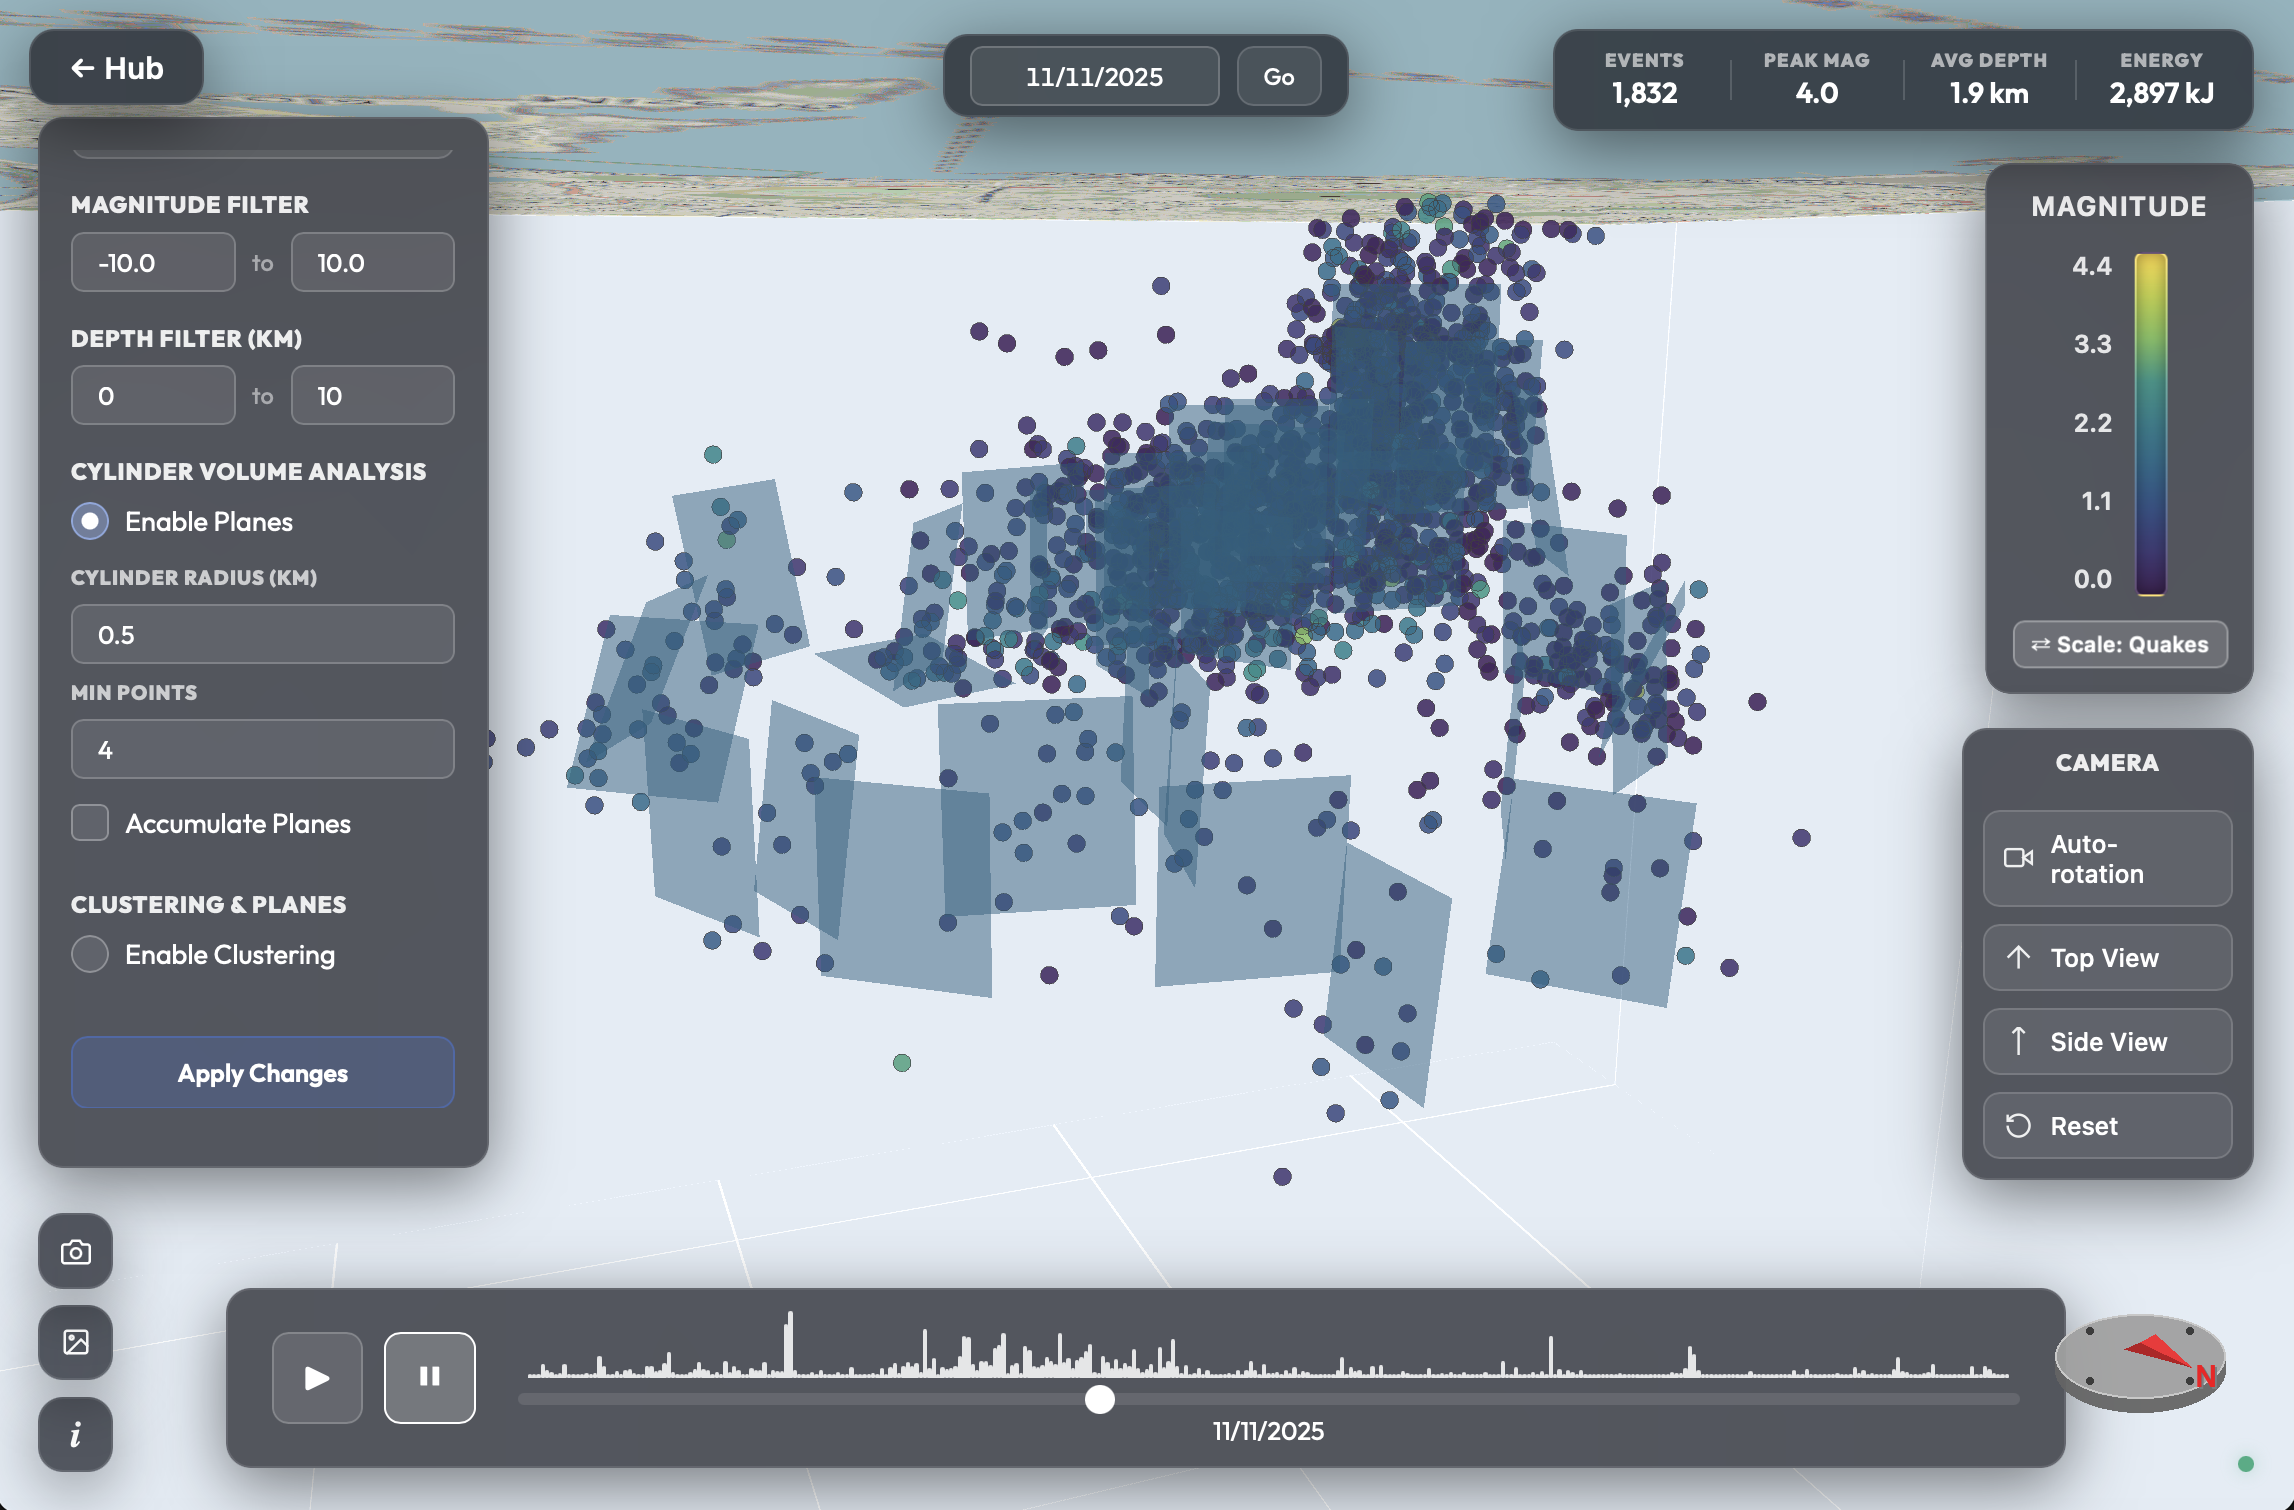
\includegraphics[width=\textwidth]{images/animated_visualization_cylinder_planes.png}
\caption{Dynamic cylinder grid partitioning with automated structural plane fitting during 4D evolution.}
\label{fig:anim-cylinder-planes}
\end{subfigure}
\caption{The 4D Animated Spatio-Temporal View workflow. Users configure parameters via the dialog (\subref{fig:anim-menu}), explore time-evolving seismicity (\subref{fig:anim-viz}), and observe automated fault plane tracking (\subref{fig:anim-cylinder-planes}).}
\label{fig:anim-multi}
\end{figure}

Prior to starting the animation, the time parameters (such as step size and frame rate) are configured via a dedicated dialog window (\Cref{fig:anim-menu}). The resulting 4D view (\Cref{fig:anim-viz}) allows interactive exploration of the chronological sequence. In addition, the volume can be partitioned into a spatial grid of vertical cylinders (\Cref{fig:anim-cylinder-planes}). This subdivision was implemented to better understand the spatial distribution of the data, as partitioning the volume isolates and subdivides the fault geometry into local, simpler planar segments. As earthquakes occur inside these cylinders, the system dynamically calculates and renders these local structural fault planes in real-time, allowing users to visualise how seismic events evolve over time across the identified planar structures.

\section{3D Cluster Analysis View}
\label{sec:view-cluster}

The cluster analysis mode integrates spatial machine learning with structural geological modelling.

\subsection{Cluster Visualisation and Interactive Tuning}

To provide a comprehensive geometrical understanding of seismogenic structures, Seismic Viewer renders every identified cluster through four complementary representations within the 3D WebGL scene. These representations address different analytical needs: boundary delineation, volumetric extent, structural orientation, and individual event membership. Together, they allow researchers to examine a cluster from multiple geometric perspectives simultaneously.
\begin{enumerate}
    \item \textbf{Wireframe Convex Hulls (\texttt{Scatter3d})}: Outer boundary envelopes highlighting the spatial footprint and volumetric extent of each distinct cluster.
    \item \textbf{Triangulated Solid Meshes} (\texttt{Mesh3d}, with \texttt{alphahull=0}): Smooth, semi-transparent volumetric convex hulls enclosing the clusters.
    \item \textbf{Structural Fault Planes (\texttt{Mesh3d})}: Planar surfaces calculated via RANSAC robust estimation coupled with Singular Value Decomposition (SVD) refinement. Each plane displays orientation vectors alongside precise geological strike and dip angles upon mouse hover.
    \item \textbf{Clustered Event Spheres}: Discrete event spheres coloured by cluster label using categorical palettes, with unclustered background noise explicitly assigned neutral grey.
\end{enumerate}
When users interactively adjust spatial clustering hyperparameters, such as neighbourhood radius $\varepsilon$, minimum samples threshold \texttt{min\_samples}, or cluster count $K$, via the side control panel, the frontend dispatches a \texttt{get\_cluster\_update} WebSocket message. The Python backend asynchronously recomputes cluster labels and structural planes without blocking the event loop, returning the newly generated Plotly trace definitions. The frontend then replaces the existing traces in the WebGL scene, thereby updating the visualisation while preserving the user's current camera perspective.

\subsection{Sub-Clustering}
\label{sec:sub-clustering}

To analyse hierarchical structures, researchers can perform secondary sub-clustering on specific data subsets. By utilizing the \textbf{locked clusters} feature, users can preserve previously identified and validated groups. The algorithm will then selectively re-analyse and sub-divide all the remaining unlocked clusters simultaneously. The refined results can subsequently be applied back to merge cleanly into the parent view.

\Cref{fig:cluster-multi} provides an overview of the clustering tools. \Cref{fig:cluster-viz} shows the standard 3D clustering interface. \Cref{fig:anim-clustering-noplanes} displays how clustering evolves over time. To ensure visual consistency, a tracking algorithm guarantees that each cluster maintains the same colour across all animation frames. Finally, \Cref{fig:anim-clustering-planes} and \Cref{fig:anim-clustering-unified} combine the animated clusters with dynamically calculated fault planes and spatial cylinders. This combination allows researchers to observe how geological structures evolve and rotate over time.

\begin{figure}[H]
\centering
\begin{subfigure}{0.95\textwidth}
\centering
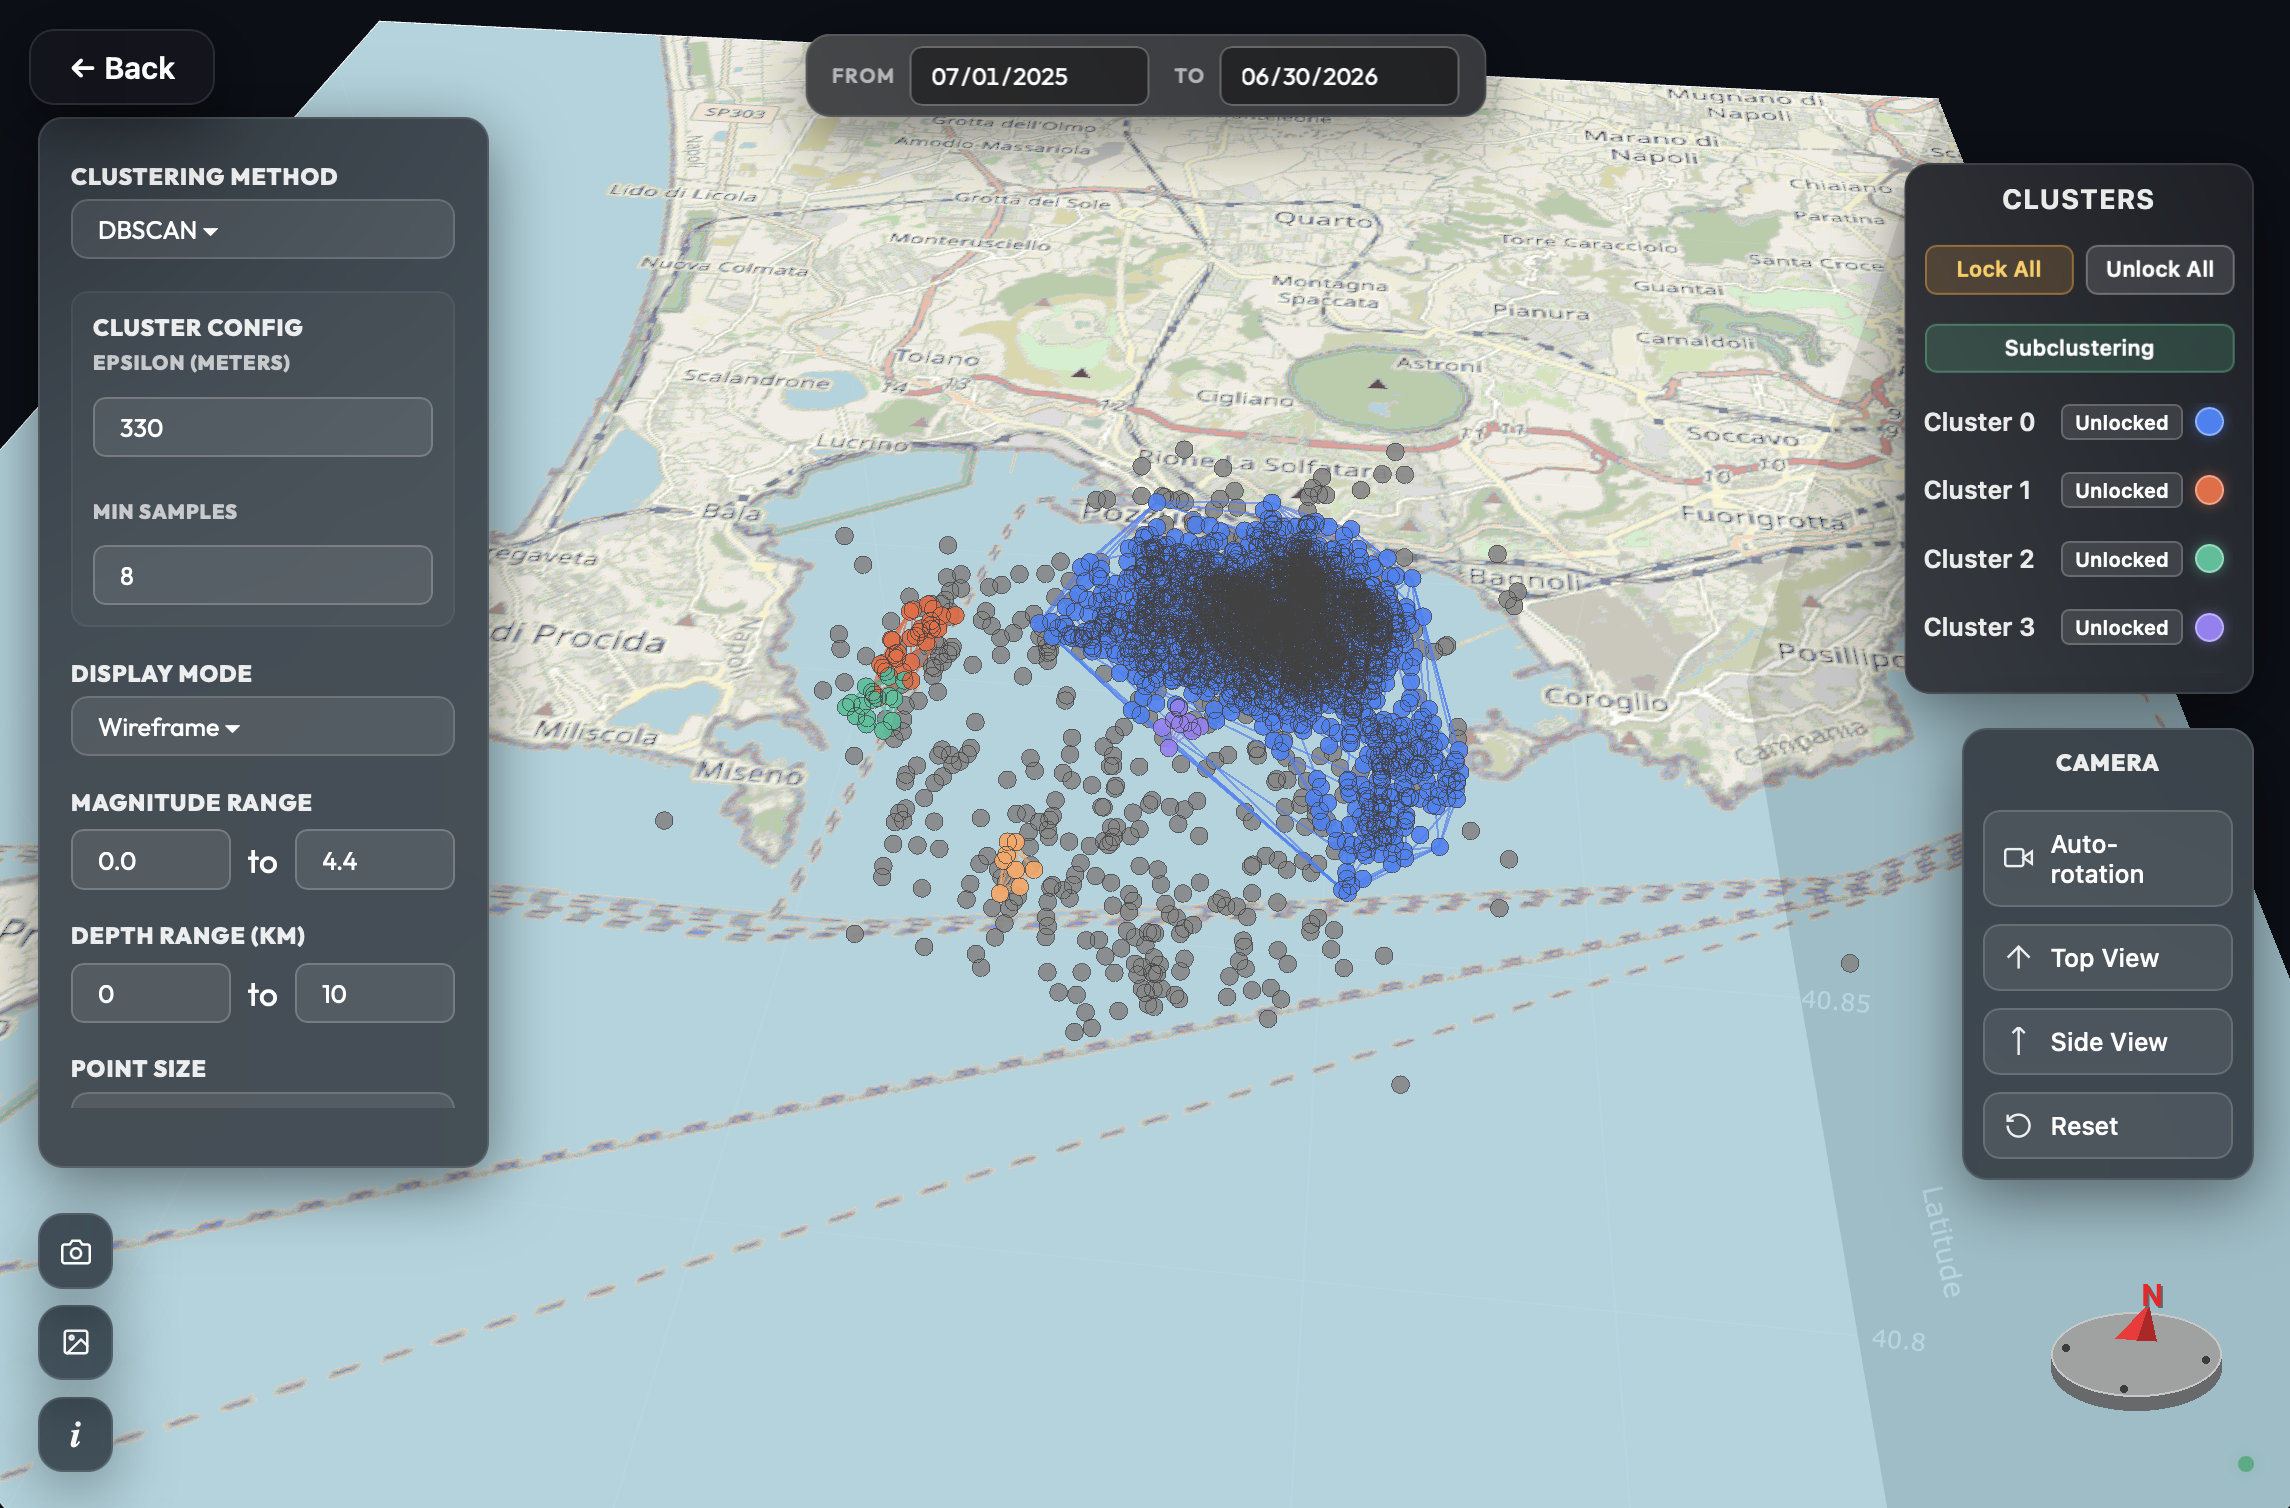
\includegraphics[width=\textwidth]{images/clustering_visualization.png}
\caption{Static 3D workspace with hulls and planes.}
\label{fig:cluster-viz}
\end{subfigure}

\vspace{3mm}
\begin{subfigure}{0.95\textwidth}
\centering
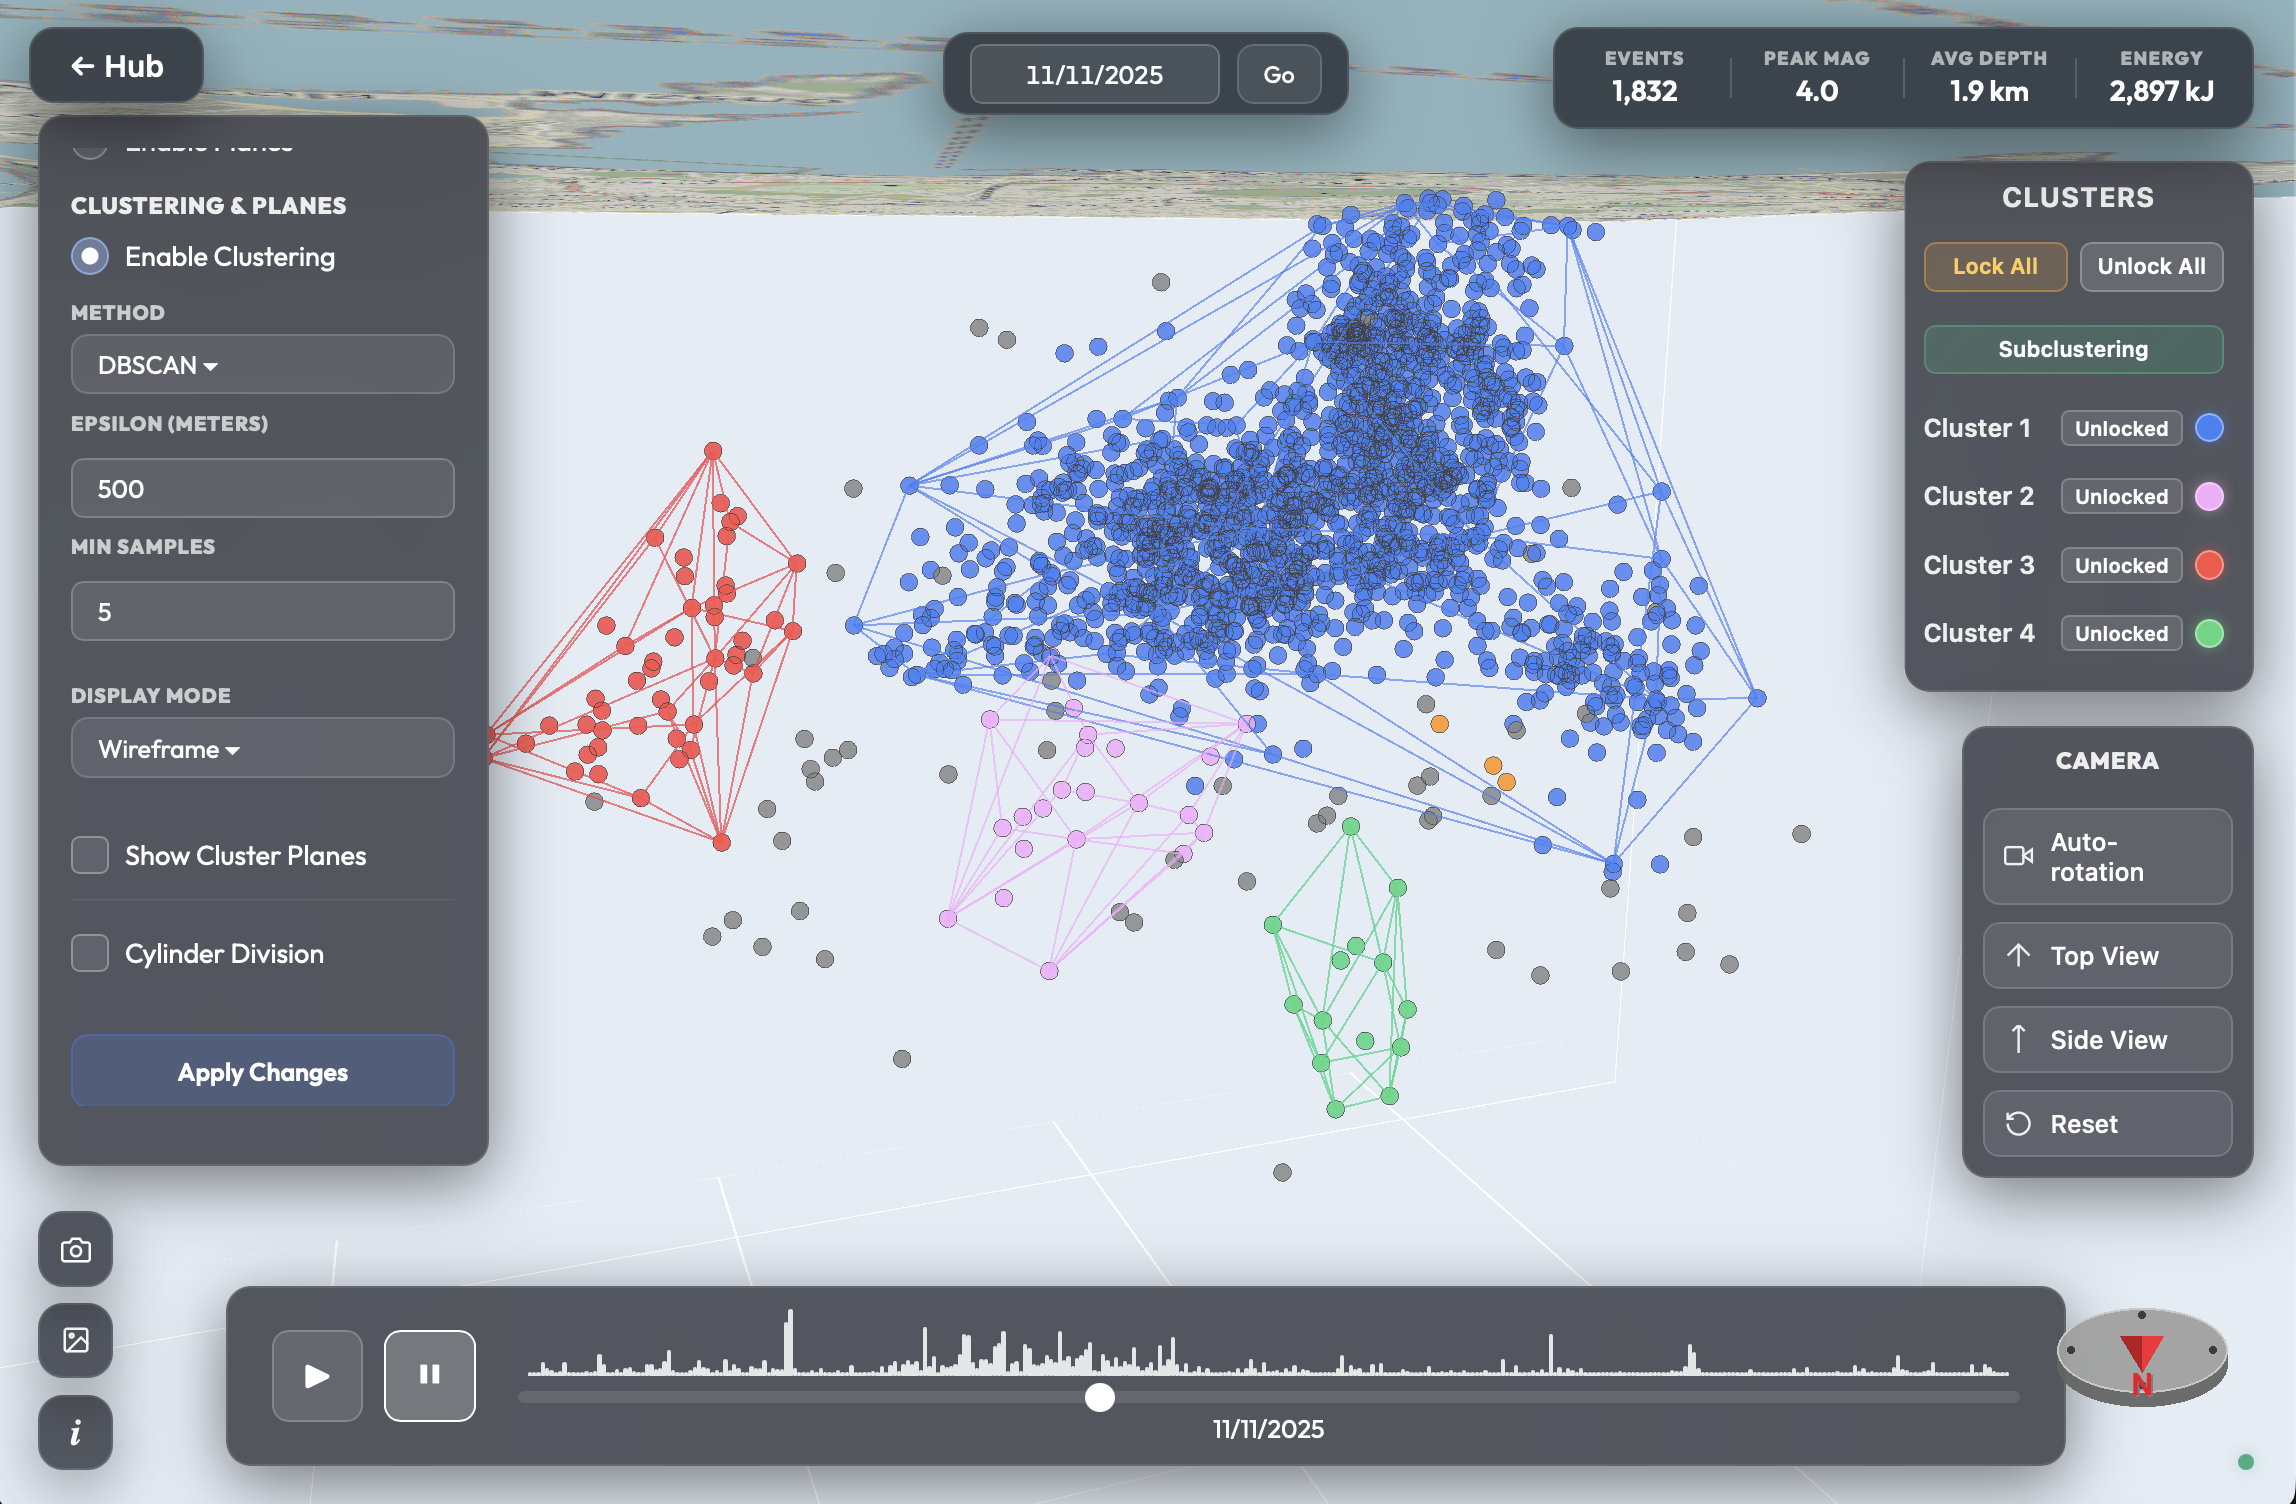
\includegraphics[width=\textwidth]{images/animated_clustering_without_planes.png}
\caption{Animated clustering with Global Label Matching.}
\label{fig:anim-clustering-noplanes}
\end{subfigure}
\caption{Multi-scale static (\subref{fig:cluster-viz}) and animated (\subref{fig:anim-clustering-noplanes} to \subref{fig:anim-clustering-unified}) 3D/4D Cluster Analysis modes (Part 1).}
\end{figure}

\begin{figure}[H]
\ContinuedFloat
\centering
\begin{subfigure}{0.95\textwidth}
\centering
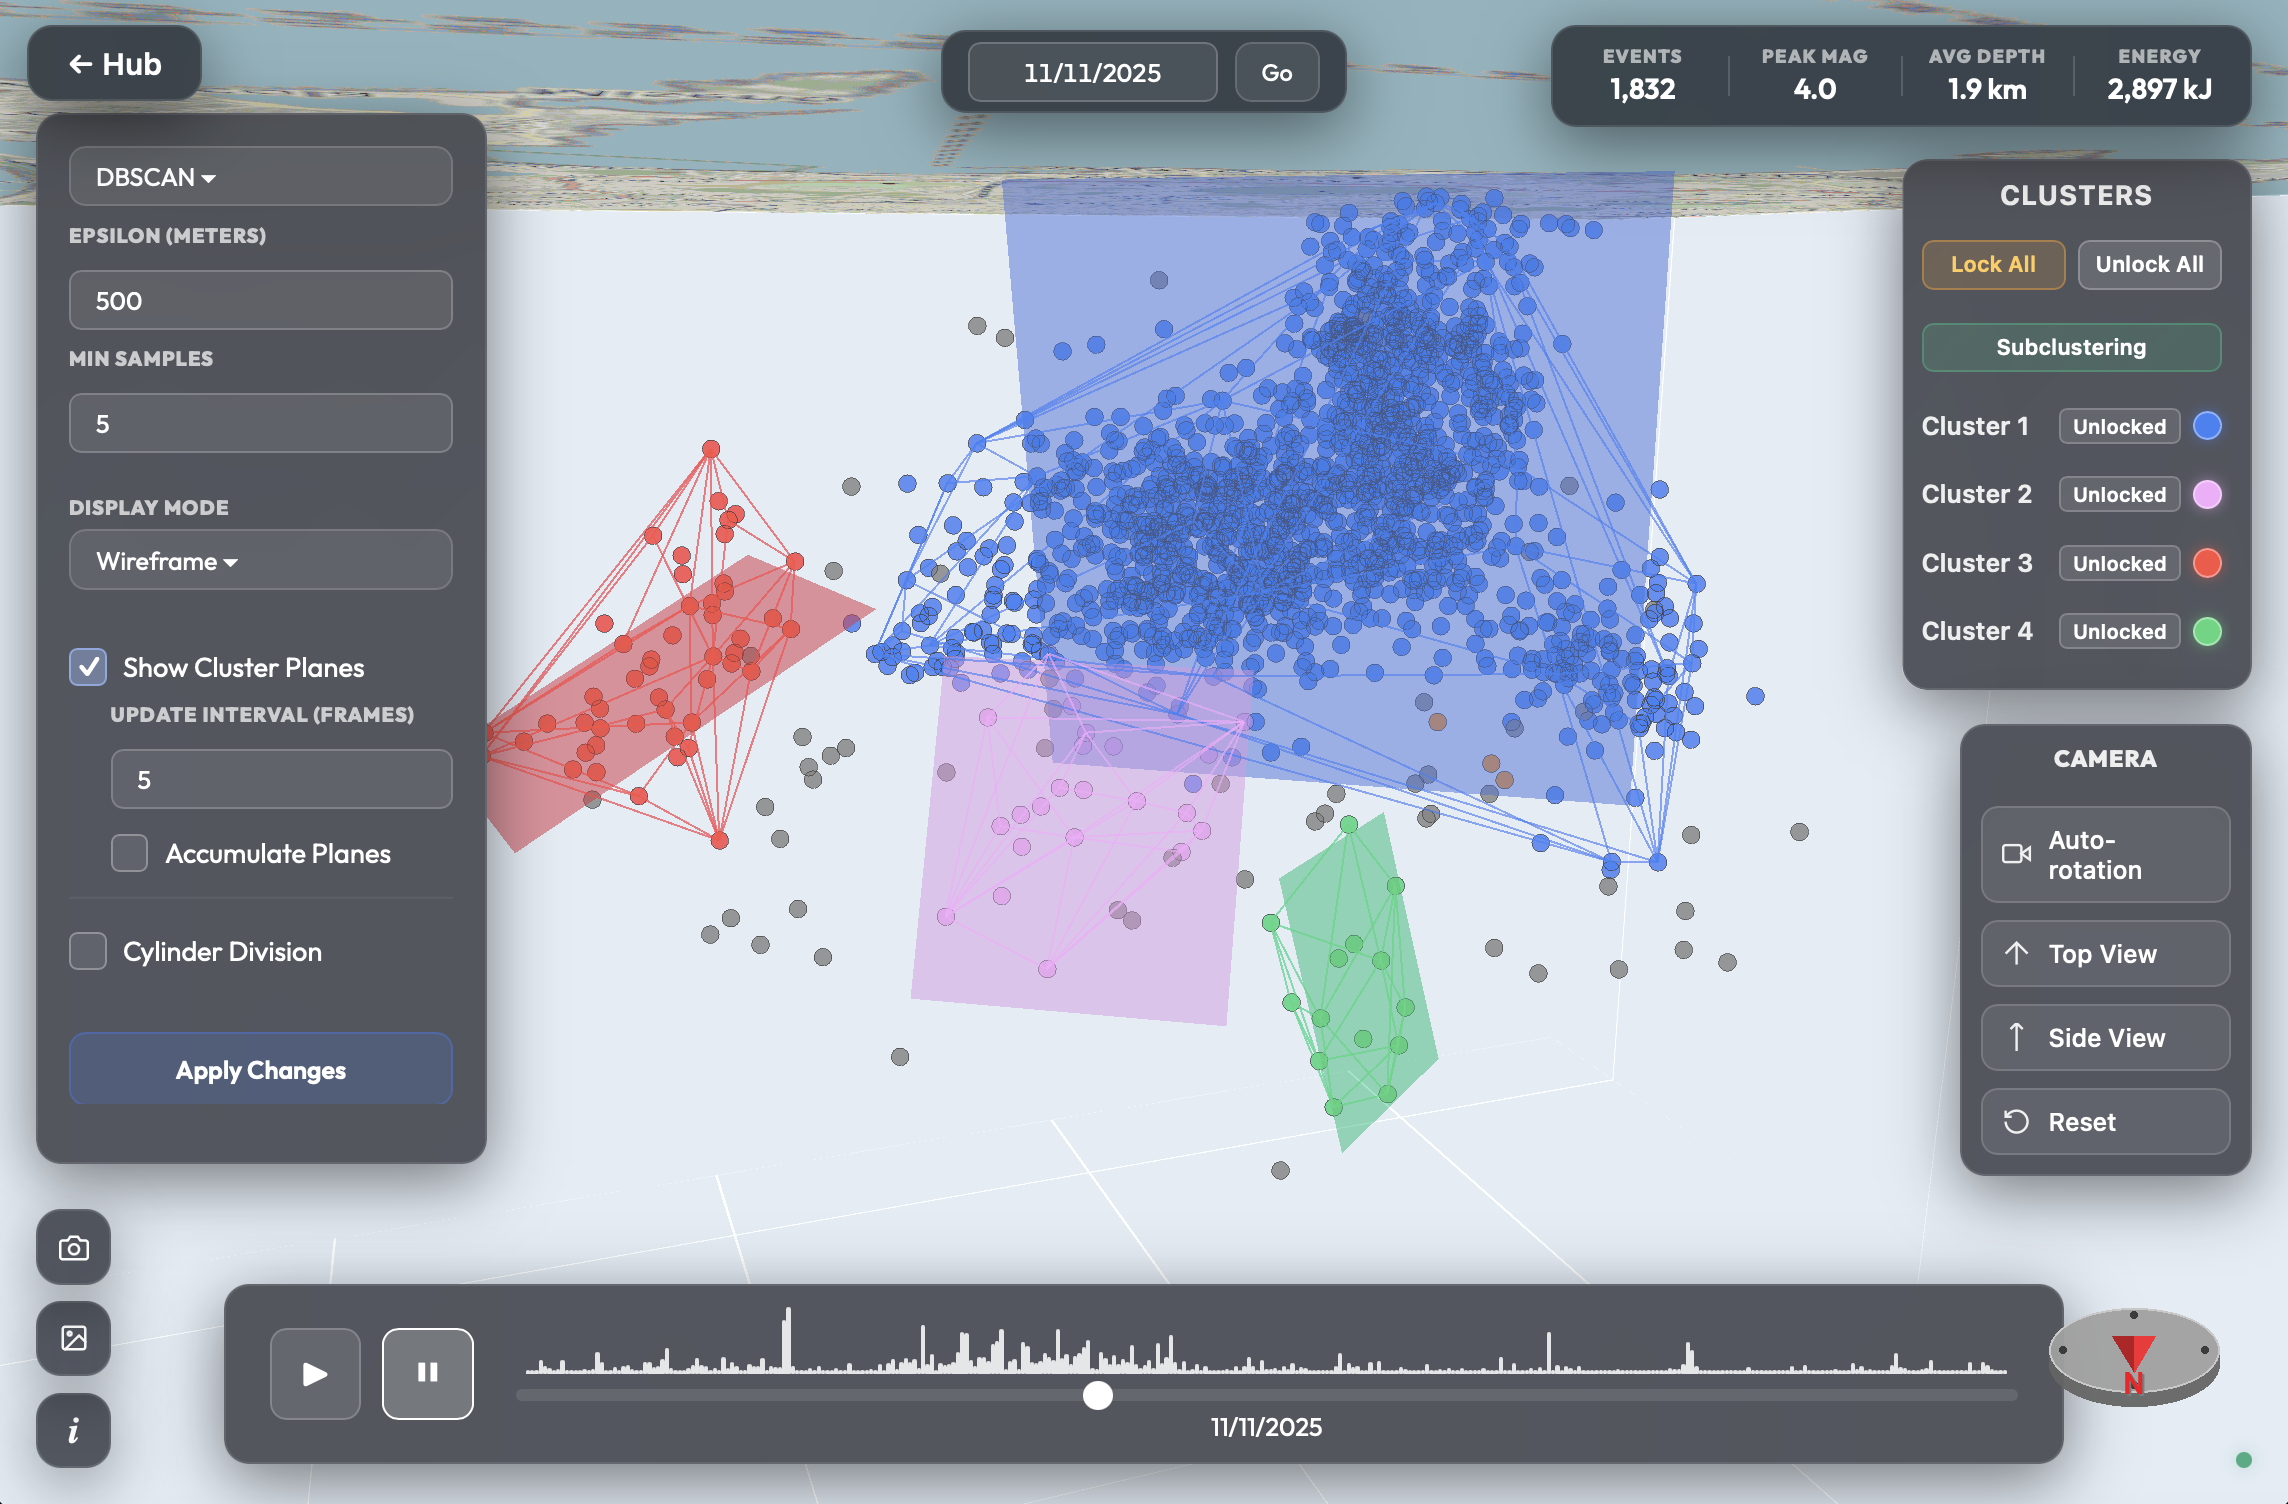
\includegraphics[width=\textwidth]{images/animated_clustering_with_planes.png}
\caption{Animated clustering with RANSAC+SVD planes.}
\label{fig:anim-clustering-planes}
\end{subfigure}

\vspace{3mm}
\begin{subfigure}{0.95\textwidth}
\centering
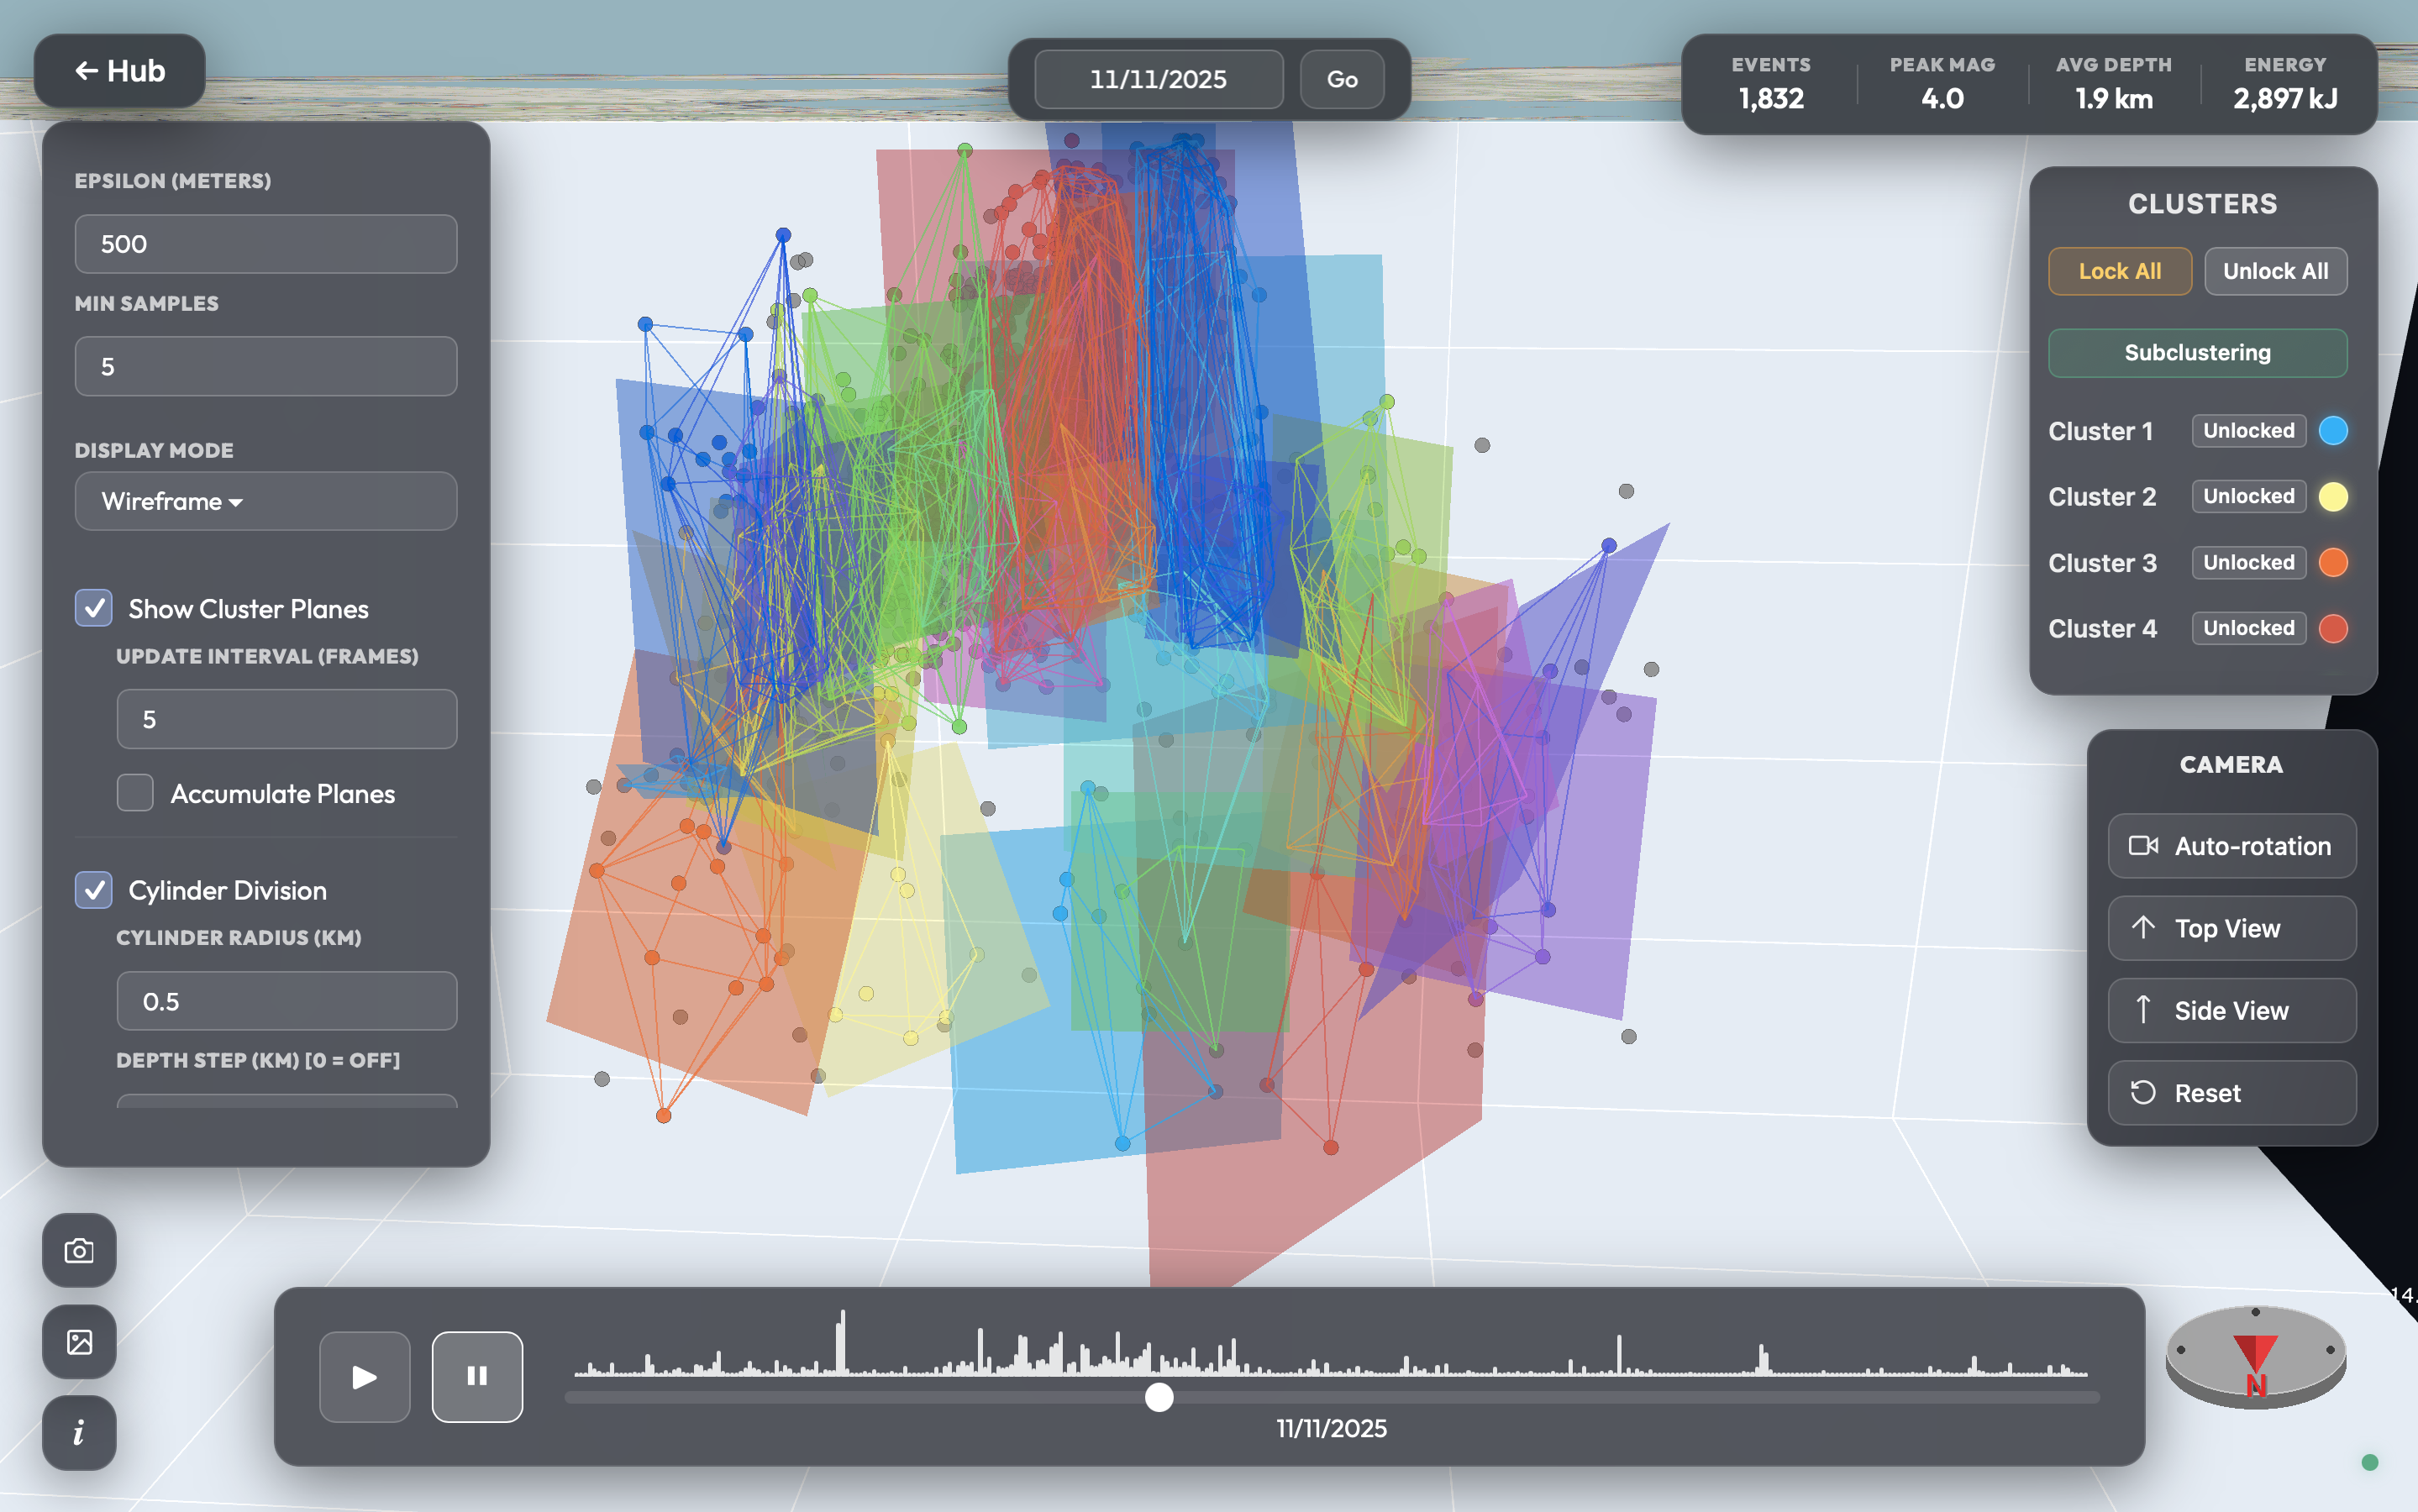
\includegraphics[width=\textwidth]{images/animated_clustering_planes_cylinder.png}
\caption{Unified 4D cylinder partitioning and plane fitting.}
\label{fig:anim-clustering-unified}
\end{subfigure}
\caption{Multi-scale static (\subref{fig:cluster-viz}) and animated (\subref{fig:anim-clustering-noplanes} to \subref{fig:anim-clustering-unified}) 3D/4D Cluster Analysis modes (Part 2).}
\label{fig:cluster-multi}
\end{figure}

\section{Additional Data Layers \& View Caching}
\label{sec:additional-layers}

\subsection{Auxiliary Layers: Tomography, Uplift, and Stations}
\label{sec:tomography}
\label{sec:uplift}
\label{sec:stations}

Seismic Viewer integrates three auxiliary data layers, processed through the \texttt{core/\allowbreak layer\_utils.py} module:
\begin{itemize}
    \item \textbf{Seismic Tomography ($V_p/V_s$ Ratio)}: The raw tomographic data, originally provided in UTM Zone~33N coordinates, is converted to geographic coordinates and projected into physical metric kilometres $(x, y, z)_\text{km}$ using equatorial conversion factors ($k_x = K \cos(\bar{\phi})$, $k_y = K$, depths in km). Because measurements only exist at specific surveyed points, the software estimates values across a regular $30 \times 22 \times 16$ volumetric grid using \textit{Inverse Distance Weighting}. The value of any grid point is calculated as a weighted average of its $k=16$ nearest known neighbours in Euclidean distance ($d$, in physical kilometres), scaling inversely with the square of the distance ($p=2$):
    \begin{equation}
        V(\mathbf{x}) = \frac{\sum_{i=1}^{k} w_i \cdot V_i}{\sum_{i=1}^{k} w_i}, \quad w_i = \frac{1}{d(\mathbf{x}, \mathbf{x}_i)^2}
        \label{eq:idw}
    \end{equation}
    To prevent mathematical artefacts in regions far from observation points, the system applies a distance-decay function. As the distance $d_\text{min}$ (in kilometres) to the nearest station increases, this function smoothly blends the estimated value back into the standard crustal background value ($1.75$):
    \begin{equation}
        V_\text{final}(\mathbf{x}) = \alpha(\mathbf{x}) \cdot V_\text{IDW}(\mathbf{x}) + (1 - \alpha(\mathbf{x})) \cdot 1.75
        \label{eq:gaussian-damping}
    \end{equation}
    where $\alpha(\mathbf{x}) = \exp(-(d_\text{min}/\sigma)^2)$ with characteristic decay radius $\sigma = 2.0$~km acts as the blending weight, decreasing smoothly from 1 (near known data) to 0 (far away), matching the station spacing of the volcanic network.
    \item \textbf{GNSS Ground Deformation (Uplift)}: To visualise ground movement, the system reads historical displacement records and matches them with permanent monitoring stations. To estimate vertical displacement across the entire caldera, the software interpolates values onto a $30 \times 30$ surface grid in metric kilometre coordinates using an IDW weighting exponent of $p=2.5$, modeling the rapid spatial decay characteristic of elastic half-space deformation. The result is displayed on the map either as a coloured 2D surface or as 3D columns rising above the surface.
    \item \textbf{Monitoring Stations}: Permanent station positions are plotted as labelled markers, aiding spatial evaluation of catalogue completeness thresholds.
\end{itemize}

These three auxiliary layers serve complementary roles in the interpretation workflow. By overlaying tomographic anomalies and ground deformation patterns onto the same 3D scene as the earthquake hypocentres, researchers can visually assess whether seismic swarms correlate with known velocity anomalies or with areas of maximum surface uplift, providing a more integrated understanding of the underlying volcanic processes.

\subsection{View Caching and Navigation}
\label{sec:view-caching}

To ensure faster navigation between complex workspaces, the backend bridge maintains an in-memory view cache (\texttt{\_html\_store}, bounded to 4 entries via FIFO eviction) keyed by a composite tuple of file path, view style, animation/windowing parameters, clustering configuration, and locked cluster states. A navigation history stack (\texttt{\_history\_stack}) allows instantaneous back and forward navigation in the clustering view while preserving exact parameter context.

\subsection{Export Engine and Interoperability}
\label{sec:export}

To support external workflows and reporting, Seismic Viewer provides an export subsystem implemented across \texttt{core/exporter.py} and \texttt{assets/viz\_export.js}. Researchers can export filtered catalogues and identified cluster subsets into multiple formats:
\begin{itemize}
    \item \textbf{Structured CSV}: Exports hypocentral coordinates, magnitudes, and timestamps, prefixed with a metadata comment documenting the clustering algorithm and hyperparameters used.
    \item \textbf{GeoJSON}: Formats cluster points into a standard \texttt{FeatureCollection} with geographic point geometries and properties, enabling direct import into external GIS applications such as QGIS.
    \item \textbf{High-Resolution Graphics}: Captures the active WebGL canvas via \texttt{Plotly.\allowbreak toImage}, generating publication-quality PNG renderings.
\end{itemize}

% ══════════════════════════════════════════════════════════════════════
% CHAPTER 7: DEVELOPMENT PROCESS & CHALLENGES
% ══════════════════════════════════════════════════════════════════════

\chapter{Development Process and Challenges}
\label{ch:development}

This chapter documents the software engineering process behind Seismic Viewer, detailing the development timeline, the iterative implementation methodology, major technical challenges and key architectural decisions.

\section{Development Timeline \& Iterative Methodology}
\label{sec:timeline}
\label{sec:methodology}

The project evolved through continuous iterations. As depicted in \Cref{fig:timeline}, development progressed through six distinct phases: (1)~3D visualization prototyping, (2)~pywebview bridge integration and clustering, (3)~UI/UX redesign and INGV API integration, (4)~binary streaming and cylinder grid implementation, (5)~integration of tomography and GNSS station layers, and (6)~modular package refactoring and testing.

\begin{figure}[htbp]
\centering
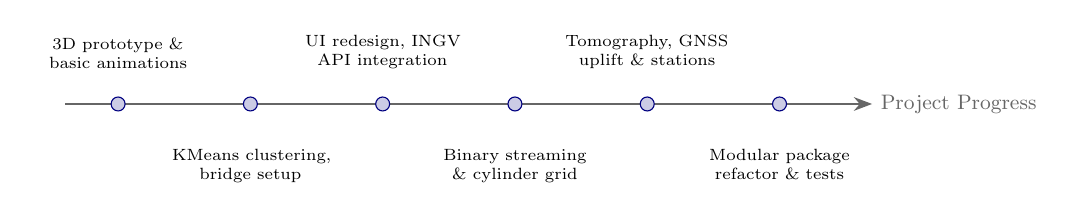
\begin{tikzpicture}[
    milestone/.style={circle, draw=NavyBlue, fill=NavyBlue!20, inner sep=2pt, minimum size=6pt},
    desc/.style={font=\scriptsize, text width=2.5cm, align=center},
    scale=0.84, transform shape
]
\draw[thick, -Stealth, black!60] (0,0) -- (12.2,0) node[right, font=\small] {Project Progress};

\node[milestone] (m1) at (0.8,0) {}; \node[desc, above=0.3cm of m1] {3D prototype \& basic animations};
\node[milestone] (m2) at (2.8,0) {}; \node[desc, below=0.45cm of m2] {KMeans clustering, bridge setup};
\node[milestone] (m3) at (4.8,0) {}; \node[desc, above=0.3cm of m3] {UI redesign, INGV API integration};
\node[milestone] (m4) at (6.8,0) {}; \node[desc, below=0.45cm of m4] {Binary streaming \& cylinder grid};
\node[milestone] (m5) at (8.8,0) {}; \node[desc, above=0.3cm of m5] {Tomography, GNSS uplift \& stations};
\node[milestone] (m6) at (10.8,0) {}; \node[desc, below=0.45cm of m6] {Modular package refactor \& tests};
\end{tikzpicture}
\caption{Development milestones highlighting the iterative implementation methodology.}
\label{fig:timeline}
\end{figure}

\revised{The software was built using an iterative workflow, with features prototyped and refined through continuous feedback. As the application expanded, the codebase was refactored twice: first by splitting a monolithic script into a modular package, and later by introducing FastAPI and WebSockets for data streaming.}

\section{Key Technical Challenges and Solutions}
\label{sec:challenges}

\greenrevised{Developing a high-performance, desktop-grade seismological analysis application combining a native Python runtime with a modern browser-based rendering engine presented significant software engineering challenges. This section analyses the primary technical bottlenecks encountered during development, the architectural and algorithmic solutions designed to overcome them, and their practical impact on system stability and responsiveness.}

\subsection{Rendering Performance and UX Optimisation}
\label{sec:challenge-camera}
\label{sec:challenge-binary}
\label{sec:challenge-flash}
\label{sec:challenge-webgl}

\greenrevised{The graphical user interface must handle large, multi-dimensional point clouds with interactive frame rates while maintaining a smooth desktop user experience.}

\paragraph{Camera State Preservation across Dynamic Re-clustering.}
\greenrevised{In early prototypes, interactive operations such as re-clustering, parameter adjustments, or depth filtering triggered a complete view reset. Because the Plotly.js engine re-evaluates the entire 3D scene definition upon receiving updated trace collections, the virtual camera automatically snapped back to default spatial coordinates $(x=1.25, y=1.25, z=1.25)$. This disruptive behaviour disoriented domain experts who had carefully aligned the perspective with specific seismogenic fault planes. The issue was resolved by injecting persistent state tracking using the \texttt{uirevision} attribute within the figure layout (\Cref{lst:uirevision}). By maintaining \texttt{uirevision='constant'} across all subsequent updates, Plotly compares existing camera transformations against incoming scene payloads, permanently preserving user orientation, elevation, zoom level, and centre of rotation.}

\begin{lstlisting}[language=Python, caption={Camera state persistence via \texttt{uirevision}.}, label={lst:uirevision}]
fig.update_layout(
    uirevision='constant',
    scene=dict(
        uirevision='constant',
        camera=dict(eye=dict(x=1.25, y=1.25, z=1.25), center=dict(x=0, y=0, z=0))
    )
)
\end{lstlisting}

\paragraph{JSON Deserialization Bottlenecks and Binary Streaming.}
\greenrevised{The standard web communication pattern relies on JSON serialization for tabular and numerical data exchange. However, transferring dense earthquake catalogues (exceeding 50{,}000 hypocentral events with multiple spatial and temporal attributes) exposed severe throughput limitations. In Python, serializing large NumPy arrays into textual JSON representations incurred substantial CPU overhead. More critically, the browser's JavaScript engine suffered severe main-thread blocking when parsing multi-megabyte JSON strings, instantiating tens of thousands of intermediate heap objects and dropping the rendering frame rate below 10 FPS. To eliminate this bottleneck, the architecture was redesigned around a raw Float32 binary streaming protocol (\Cref{sec:binary-protocol}). Hypocentral coordinates, cluster identifiers, and metadata scalars are flattened into a contiguous C-order binary buffer directly on the backend and transmitted over WebSocket connections. On the client side, the payload is ingested at zero-copy latency into a native \texttt{Float32Array} typed array. This architectural shift reduced payload transfer size by approximately 65\% and cut data deserialization latency from several seconds to under 15 milliseconds, sustaining smooth 60 FPS viewport interactions.}

\paragraph{WebGL Context Lifecycle and GPU Resource Management.}
\greenrevised{In an embedded WebView environment, frequent transitions between complex analytical views (2D static maps, 3D hypocentral volumes, and 4D spatiotemporal animations) risk exhausting the host GPU's available WebGL contexts. Desktop operating systems strictly limit concurrent WebGL instances per rendering process (typically between 8 and 16 contexts). When unmanaged view switches allocate new canvas elements without reclaiming previous ones, the browser engine triggers a catastrophic \texttt{webglcontextlost} error, terminating rendering entirely. To ensure robust GPU resource management, an explicit view cleanup lifecycle was implemented. Before navigating away from an active analytical workspace, the frontend invokes \texttt{Plotly.purge()} on existing chart DOM nodes, explicitly deallocating shader programs, vertex buffers, and texture bindings from GPU memory. Furthermore, 3D hypocentral markers are rendered as hardware-accelerated 2D point sprites facing the camera rather than tessellated geometric spheres, capping GPU VRAM consumption below 150~MB even during large-scale catalog visualization.}

\paragraph{White-Flash Mitigation in Embedded Navigation.}
\greenrevised{Because the desktop interface relies on a dark-mode palette tailored for high-contrast seismological visualization, standard navigation between distinct HTML views caused jarring visual flickers. During the transition interval before external stylesheets and Plotly runtime bundles finish parsing, the WebView's default white background canvas was momentarily exposed. To maintain visual continuity, a proactive dark overlay mechanism (\texttt{\_inject\_dark\_overlay()}) was integrated into the view generation pipeline. A lightweight inline script injects an opaque, dark container into the document header before any stylesheet requests are dispatched. Once the DOM content and client-side styling are fully initialized, the overlay smoothly fades out via a CSS transition, delivering an aesthetically seamless desktop transition.}

\subsection{Backend Architecture, Concurrency, and Algorithmic Resilience}
\label{sec:challenge-concurrency}
\label{sec:challenge-flickering}
\label{sec:challenge-ipc}
\label{sec:challenge-ingv}
\label{sec:challenge-memory}

\greenrevised{Managing intensive mathematical computations, asynchronous data streaming, and external web APIs within a unified desktop application required solving critical concurrency and resilience challenges.}

\paragraph{Native GUI Event Loop and Asynchronous Backend Coexistence.}
\greenrevised{A foundational software engineering hurdle in \texttt{pywebview}-based architectures is the coexistence of the native OS window loop and the asynchronous backend server. Native GUI toolkits (Cocoa on macOS, Win32/WebView2 on Windows, and GTK on Linux) demand exclusive control over the operating system's main thread to process window events, user inputs, and message queues. Simultaneously, the application backend relies on FastAPI and Uvicorn running an asynchronous \texttt{asyncio} event loop for WebSocket streaming and REST endpoints. Attempting to run both loops on the main thread results in mutual deadlocks. To resolve this, the startup lifecycle was decoupled: the FastAPI ASGI server is spawned within a dedicated daemon thread, while \texttt{pywebview.start()} retains control of the main thread. Inter-thread communication is coordinated through thread-safe asynchronous dispatchers and local HTTP/WebSocket loopback channels, ensuring that computationally intensive backend routines never starve the GUI thread of input events.}

\paragraph{Chromatic Stability in 4D Spatiotemporal Clustering.}
\greenrevised{When unsupervised clustering algorithms (such as DBSCAN or MiniBatchKMeans) are evaluated independently on consecutive temporal time windows during 4D animations, they assign cluster identifiers arbitrarily without historical memory. Consequently, a single continuous geological fault structure could receive label 0 in frame $t$, label 2 in frame $t+1$, and label 1 in frame $t+2$. In animated playback, this caused rapid chromatic flickering, severely hindering the geologist's ability to track fault propagation and seismic swarm migration over time. This was overcome by designing the Global Label Matching algorithm (\Cref{sec:label-matching}). By preserving a global hypocentre-to-label registry and applying majority voting across active cluster members (\Cref{eq:majority-voting}), the analytical engine re-maps local frame labels to temporally coherent global identifiers, ensuring seamless colour persistence across the entire seismic sequence.}

\paragraph{Zero-Copy Inter-Process Communication for Parallel Computation.}
\greenrevised{Computing RANSAC consensus inlier sets and SVD planar fits across hundreds of animation frames is computationally demanding. While Python's standard multithreading is constrained by the Global Interpreter Lock (GIL) for CPU-bound numerical tasks, spawning standard multi-process pools via \texttt{multiprocessing} or \texttt{concurrent.futures} introduces severe serialization overhead when passing large coordinate arrays across process boundaries. To achieve true parallel scaling without memory duplication, the backend leverages shared memory buffers (\texttt{multiprocessing.shared\_memory}). The primary coordinate array is loaded once into a shared POSIX memory segment, and lightweight integer slice references are dispatched to worker processes. This zero-copy IPC design bypasses the GIL entirely and eliminates IPC copy overhead, achieving a near-linear speedup across available CPU cores during 4D batch synthesis.}

\paragraph{Resilience against Remote INGV API Failures.}
\greenrevised{The integrated INGV GOSSIP web service exposes a REST API for querying historical earthquake catalogues. However, querying multi-year seismic sequences frequently exposed connection timeouts, rate limiting, and truncated responses for specific annual intervals. In naive implementations, a single network drop or empty payload would crash the entire ingestion pipeline. To guarantee system resilience, the online importer module (\texttt{core/online\_importer.py}) partitions large historical queries into isolated per-year asynchronous request blocks wrapped in defensive \texttt{try...except} handlers. If a specific year encounters a timeout or malformed XML/JSON payload, the importer logs a structured warning, records the missing temporal interval, and seamlessly continues fetching subsequent years. The user is presented with a complete summary of successfully ingested records alongside any flagged intervals, preventing data loss without halting application execution.}

\paragraph{Session Memory Bounding and FIFO Store Eviction.}
\greenrevised{During multi-hour exploratory research sessions, seismologists frequently generate dozens of alternative 3D views, parameter variations, and sub-cluster models. Storing all generated Plotly figures and processed dataframes in RAM caused steady memory inflation, eventually leading to process termination on memory-constrained workstations. To enforce a strictly bounded memory footprint, a dual First-In, First-Out (FIFO) eviction policy was implemented. The analytical engine restricts \texttt{\_data\_store} to a maximum of 30 active session datasets and \texttt{\_html\_store} to 15 pre-rendered analytical views. When store capacity is reached, the oldest session objects are evicted and reclaimed by the garbage collector. Additionally, the \texttt{strip\_data()} routine decouples heavy coordinate arrays from rendered HTML templates prior to caching. As a result, total application RAM usage remains strictly bounded below 500~MB even under heavy continuous usage.}

\section{Code Quality and Architecture}
\label{sec:code-quality}

\revised{The software is organised into a modular structure. The backend is written in Python with type annotations across 12 modules, while the frontend is built with JavaScript, HTML, and CSS. Data flows unidirectionally: from the application entry point (\texttt{app.py}), through the bridge and engine (\texttt{bridge.py}, \texttt{engine.py}), to utility modules (\texttt{loader.py}, \texttt{geo\_utils.py}).}

\revised{A key aspect of the architectural design is the strict isolation of caching strategies. The system uses multiple caching layers operating at different levels: persistent disk caching with \texttt{pickle} for map tiles and terrain meshes, in-memory function-level caching with \texttt{lru\_cache} for frequently accessed computations, and session-scoped stores (\texttt{\_data\_store} and \texttt{\_html\_store}) for active analytical workspaces. Keeping these caches separate prevents data inconsistency.}

This modular organisation was not the original design. As discussed in \Cref{sec:timeline}, the codebase underwent two major refactoring cycles during the internship. The first split a single monolithic script into separate modules organised by responsibility, while the second introduced the FastAPI and WebSocket infrastructure to replace the original synchronous communication model. These refactoring efforts, though time-consuming, were essential for maintaining code quality as the application grew in complexity.

\section{\revised{Testing, Verification, and Quality Assurance}}
\label{sec:testing-qa}

\revised{To ensure software reliability and maintainability, the application includes automated testing and verification routines:}

\begin{enumerate}
    \item \revised{\textbf{Unit Testing for Coordinate Conversions}: The \texttt{core/geo\_utils.py} and \texttt{core/layer\_utils.py} modules are verified against standard geographic benchmarks. Unit tests confirm that the Inverse Mercator projection (\Cref{eq:mercator}) and UTM Zone 33N transformations reconstruct coordinates with an error below 0.1~meters.}
    \item \revised{\textbf{Structural Plane Extraction Testing}: To validate the RANSAC and SVD plane fitting engine, synthetic point clouds are generated with known strike and dip angles and tested under Gaussian positional noise. The tests confirm that the estimated strike and dip angles match the ground truth within $\pm 0.5^\circ$ for noise $\sigma = 10$~m and within $\pm 2.0^\circ$ for noise $\sigma = 100$~m.}
    \item \revised{\textbf{CSV Ingestion and Format Testing}: The schema detection logic (\texttt{core/}\allowbreak\texttt{loader.py}) is tested with different CSV formats (commas vs. semicolons, decimal commas, and alternative date formats) to maintain compatibility across earthquake catalogues.}
    \item \revised{\textbf{Modular Architecture}: Two refactoring phases decomposed 2{,}800 lines of monolithic code into 12 separate Python modules and frontend assets, simplifying codebase maintenance.}
\end{enumerate}

% ══════════════════════════════════════════════════════════════════════
% CHAPTER 8: CONCLUSIONS & FUTURE WORK
% ══════════════════════════════════════════════════════════════════════

\chapter{Conclusions and Future Work}
\label{ch:conclusions}

\section{Summary of Contributions}
\label{sec:contributions}

\revised{The analysis of existing seismic visualisation tools presented in \Cref{sec:related-tools} revealed a persistent gap in the available software landscape: no single application combined interactive 3D rendering, temporal animation, automated clustering, and structural geological analysis within an accessible desktop environment. Seismic Viewer was designed to fill precisely this gap. The contributions of this project can be grouped into three main areas: software architecture, data visualisation, and automated analysis.}

\revised{From an architectural perspective, the most significant contribution is the dual-engine design that separates computation from presentation (\Cref{ch:architecture}). By coupling a pywebview \cite{pywebview} native window with a high-throughput FastAPI \cite{fastapi} local server, the application achieves full desktop integration (native file dialogs, window management) without the memory overhead that a framework such as Electron \cite{electron} would impose. This separation is important because it allows the scientific Python backend to perform heavy numerical operations independently from the user interface, preventing the graphical environment from freezing during long calculations. A second architectural contribution is the custom binary streaming protocol, which packs numerical arrays into contiguous Float32 buffers and reduces the data transfer volume by approximately $90\%$ compared to traditional JSON serialisation. This improvement was essential for achieving fluid interactivity, as the original JSON-based approach caused the browser engine to freeze for several hundred milliseconds when parsing large catalogues.}

\revised{In the area of data visualisation, Seismic Viewer introduces a multi-modal rendering system comprising four complementary views: 2D geospatial maps, 3D static hypocentral distributions, 4D time-animated sequences, and interactive cluster analysis workspaces. The 4D animation mode, in particular, represents a novel contribution for desktop seismological tools. It allows researchers to observe how earthquake sequences evolve over time through three distinct temporal windowing strategies (accumulation, sliding window, and block mode), providing insights into migration patterns and the progressive activation of fault segments that would remain invisible in static representations. Additionally, the integration of auxiliary geophysical layers (seismic tomography cubes, GNSS vertical displacement grids, and monitoring station positions) enables researchers to correlate seismicity with deeper crustal processes within a single coherent spatial environment.}

\revised{The third area of contribution concerns the automated structural analysis pipeline. Seismic Viewer implements three complementary clustering approaches, DBSCAN \cite{ester1996dbscan}, MiniBatchKMeans \cite{lloyd1982kmeans}, and a custom cylinder grid partitioning method, each suited to different analytical scenarios. The cylinder partitioning strategy, in particular, was developed specifically for this application to ensure stable cluster assignments during 4D temporal animations without the colour swapping that affects standard unsupervised algorithms across independent frames. On top of these clustering methods, the application automatically fits structural fault planes using a two-stage RANSAC \cite{fischler1981ransac} and SVD \cite{shakarji1998least} pipeline, directly computing geologically meaningful parameters such as dip, dip direction, and strike. This combination of clustering and plane fitting within an interactive, real-time environment allows researchers to identify and characterise seismogenic structures without resorting to external analytical software.}

\section{Validation and Quantitative Performance Assessment}
\label{sec:validation}

\revised{The system was evaluated using the dense INGV Campi Flegrei caldera catalogue, comprising approximately 30,000 located earthquakes recorded between 2005 and 2024 \cite{ingv}. This dataset was chosen because its complex shallow fracturing and intense bradyseismic swarms provide a demanding test case for both the rendering pipeline and the analytical algorithms. Quantitative profiling confirmed that Seismic Viewer achieves consistent rendering performance between 60 and 120 frames per second on standard desktop hardware (M-series Apple Silicon and NVIDIA RTX GPUs) when visualising datasets exceeding 50,000 simultaneous points.}

\subsection{\revised{Experimental Benchmarks: Serialization and Streaming}}

\revised{To evaluate the Float32 binary protocol against JSON serialization, benchmarks were run across four dataset sizes ($N \in \{1{,}000, 10{,}000, 30{,}000, 50{,}000\}$ events). As reported in \Cref{tab:bench-serialization}, the Float32 format reduces payload sizes by approximately 84\% and decoding times from 824~ms to 4.2~ms for 50{,}000 events.}

\begin{table}[htbp]
\centering
\caption{\revised{Serialization benchmark: JSON vs. Float32 Binary buffer.}}
\label{tab:bench-serialization}
\footnotesize
\color{red}
\renewcommand{\arraystretch}{1.15}
\begin{tabularx}{\textwidth}{@{}r r r r r r@{}}
\toprule
\textbf{Events ($N$)} & \textbf{JSON Size} & \textbf{Float32 Size} & \textbf{Compression} & \textbf{JSON Parse} & \textbf{Float32 Parse} \\
\midrule
1{,}000   & 142~KB   & 24~KB   & 83.1\% & 14~ms  & 0.4~ms \\
10{,}000  & 1.48~MB  & 235~KB  & 84.1\% & 138~ms & 1.1~ms \\
30{,}000  & 4.46~MB  & 704~KB  & 84.2\% & 465~ms & 2.6~ms \\
50{,}000  & 7.52~MB  & 1.17~MB & 84.4\% & 824~ms & 4.2~ms \\
\bottomrule
\end{tabularx}
\end{table}

\subsection{\revised{Clustering Latency and Algorithmic Throughput}}

\revised{Execution times for the three clustering methods were measured across catalog sizes. As shown in \Cref{tab:bench-clustering}, MiniBatchKMeans and Cylinder Partitioning execute in under 80~ms for 50{,}000 events, while DBSCAN requires 382~ms.}

\begin{table}[htbp]
\centering
\caption{\revised{Clustering execution latency benchmark across dataset scales.}}
\label{tab:bench-clustering}
\footnotesize
\color{red}
\renewcommand{\arraystretch}{1.15}
\begin{tabularx}{\textwidth}{@{}r X X X@{}}
\toprule
\textbf{Events ($N$)} & \textbf{DBSCAN ($\varepsilon=300$m)} & \textbf{MiniBatchKMeans ($K=6$)} & \textbf{Cylinder Grid ($60\times50$)} \\
\midrule
1{,}000   & 6.2~ms   & 3.8~ms  & 1.9~ms \\
10{,}000  & 48.5~ms  & 18.2~ms & 8.4~ms \\
30{,}000  & 194.0~ms & 46.1~ms & 22.7~ms \\
50{,}000  & 382.0~ms & 78.4~ms & 39.1~ms \\
\bottomrule
\end{tabularx}
\end{table}

\subsection{\revised{Synthetic Validation of Structural Plane Extraction}}

Because the true position and orientation of underground faults cannot be directly observed, the plane fitting algorithms (RANSAC and SVD) were validated using synthetic datasets where the exact geometric structures were known. These datasets were generated by mathematically defining 3D planes of points at specific strike and dip angles, and subsequently introducing random Gaussian noise and scattered outliers to simulate realistic seismic measurement errors. 

\revised{As reported in \Cref{tab:bench-synthetic}, the two-stage RANSAC+SVD pipeline estimates plane orientations consistently: with noise standard deviation $\sigma = 100$~meters and 30\% background outliers, the Mean Absolute Error (MAE) is $1.42^\circ$ for Dip and $1.85^\circ$ for Strike.}

\begin{table}[htbp]
\centering
\caption{\revised{Synthetic plane estimation accuracy under Gaussian positional noise.}}
\label{tab:bench-synthetic}
\footnotesize
\color{red}
\renewcommand{\arraystretch}{1.15}
\begin{tabularx}{\textwidth}{@{}r r X X X@{}}
\toprule
\textbf{Noise $\sigma$ (m)} & \textbf{Outliers (\%)} & \textbf{Dip MAE ($^\circ$)} & \textbf{Strike MAE ($^\circ$)} & \textbf{Planarity ($P$)} \\
\midrule
10~m   & 10\% & $0.18^\circ$ & $0.24^\circ$ & 0.94 \\
25~m   & 15\% & $0.41^\circ$ & $0.56^\circ$ & 0.88 \\
50~m   & 20\% & $0.78^\circ$ & $0.99^\circ$ & 0.79 \\
100~m  & 30\% & $1.42^\circ$ & $1.85^\circ$ & 0.65 \\
\bottomrule
\end{tabularx}
\end{table}

In parallel, the global label matching algorithm (\Cref{sec:label-matching}) successfully eliminated temporal colour flickering across 4D animated cluster sequences while maintaining fast computation times, confirming its suitability for interactive exploration workflows.

\section{Future Research and Architectural Extensions}
\label{sec:future-work}

While Seismic Viewer achieves interactive responsiveness for current regional catalogues, several areas present opportunities for future development.

As dataset sizes continue to grow beyond the regional scale, the current Plotly.js \cite{plotlyjs} rendering pipeline may reach its practical limits. Migrating the frontend to specialised geospatial rendering engines, such as Deck.gl or a custom WebGL pipeline built on Three.js, could enable progressive level-of-detail rendering techniques. This migration would not only increase the maximum number of renderable points but also open the possibility of deploying the application as a fully browser-based web service, eliminating the need for local installation.

A second important direction concerns real-time monitoring integration. The current architecture analyses static or periodically updated catalogues, but integrating continuous data streaming protocols such as SeedLink or FDSN web services could transform the system into a live surveillance dashboard suitable for monitoring rooms. This would require extending the WebSocket communication layer to handle continuous data ingestion alongside the existing analytical pipeline.

Finally, future iterations could expand the analytical capabilities by integrating focal mechanism visualisations to represent fault kinematics directly in the 3D scene, as well as Coulomb static stress transfer maps to analyse how individual earthquakes redistribute tectonic stress across neighbouring faults.

\section{Concluding Remarks}
\label{sec:concluding}

\revised{Seismic Viewer demonstrates combining web technologies with Python libraries for geophysical analysis. The hybrid architecture separating the Python backend from the WebGL frontend balanced computation speed with development workflow. Python libraries (NumPy \cite{numpy2020}, scikit-learn \cite{pedregosa2011sklearn}) provide numerical routines, while the web frontend delivers GPU-accelerated 3D graphics.}

\revised{The iterative methodology aligned software capabilities with research requirements. Feedback from domain experts at INGV Osservatorio Vesuviano and Roma Tre University guided features such as sub-clustering and cylinder partitioning.}

\revised{This work supports the transition from static plots toward interactive exploration in seismology. By providing 4D visualization and clustering in a desktop application, Seismic Viewer offers a foundation for studying seismogenic structures and monitoring volcanic unrest at Campi Flegrei \cite{desiena2017bradyseism, giordano2025birth}.}


\appendix
% ══════════════════════════════════════════════════════════════════════
% APPENDIX A: SUPPLEMENTARY TECHNICAL DETAILS
% ══════════════════════════════════════════════════════════════════════

\chapter{Supplementary Technical Details}
\label{app:technical_details}

This appendix provides a formal specification of the data structures and the core algorithmic logic utilized within Seismic Viewer. Standardizing the input and internal formats ensures that the system can easily parse external catalogs and efficiently render them, while the computational pipeline ensures robust data analysis. By documenting these structures and algorithms, future extensions to the software can maintain compatibility with the existing core architecture.

\section{Seismic Data Structures}
\label{sec:data_structures}

The design of Seismic Viewer places a strong emphasis on maintaining a clear separation between the external data representation and the internal state used for high-performance computation. This section outlines both formats in detail, illustrating how raw textual data is efficiently translated into numerical matrices.

\subsection{Input Catalog Format}

Seismological data must be structured in a CSV following the specifications detailed in \cref{tab:csv-schema}. The schema requires specific temporal and spatial fields to ensure correct localization within the 3D WebGL environment. To accommodate the vast amount of data often recorded during seismic swarms, the format is kept as lightweight as possible. External catalogs, such as those provided by the INGV, must be pre-processed or mapped to this standard structure before ingestion. The mandatory fields include unique identifiers, precise origin timestamps, and geographical coordinates expressed in decimal degrees.

\begin{table}[htbp]
\centering
\caption{Expected schema for input seismic catalogs.}
\label{tab:csv-schema}
\footnotesize
\renewcommand{\arraystretch}{1.15}
\begin{tabularx}{\textwidth}{@{}l l >{\raggedright\arraybackslash}X@{}}
\toprule
\textbf{Field Name} & \textbf{Data Type} & \textbf{Description} \\
\midrule
\texttt{id} & \texttt{string} & Unique identifier for the seismic event \\
\texttt{time} & \texttt{ISO 8601 string} & Origin time of the event (e.g., 2024-01-01T12:00:00) \\
\texttt{latitude} & \texttt{float} & Event epicenter latitude in WGS84 decimal degrees \\
\texttt{longitude} & \texttt{float} & Event epicenter longitude in WGS84 decimal degrees \\
\texttt{depth} & \texttt{float} & Hypocentral depth in kilometers \\
\texttt{mag} & \texttt{float} & Magnitude of the event \\
\bottomrule
\end{tabularx}
\end{table}

\subsection{Internal Application State}

Once parsed by the Python backend, the catalog is transformed into an internal state object optimized for rendering and clustering algorithms. The data is held in memory as multi-dimensional \texttt{numpy} arrays to support the matrix operations required by DBSCAN and RANSAC. Transitioning from a row-based CSV structure to a column-based array format significantly improves memory locality and cache performance during heavy numerical computations. This design choice helps achieve interactive frame rates in the application's user interface.

\begin{table}[htbp]
\centering
\caption[Internal data representation in the processing pipeline]{Internal data representation in the processing pipeline.}
\label{tab:internal-schema}
\footnotesize
\renewcommand{\arraystretch}{1.15}
\begin{tabularx}{\textwidth}{@{}l l >{\raggedright\arraybackslash}X@{}}
\toprule
\textbf{Variable} & \textbf{Type} & \textbf{Purpose} \\
\midrule
\texttt{longitude}, \texttt{latitude} & \texttt{numpy.ndarray (float32)} & Arrays of WGS84 coordinates in decimal degrees ($N$ events) \\
\texttt{depth} & \texttt{numpy.ndarray (float32)} & Array of hypocentral depths in kilometers ($N$ events) \\
\texttt{magnitude} & \texttt{numpy.ndarray} & An $N$-length array used for scaling the visual markers \\
\texttt{dates\_num} & \texttt{numpy.ndarray (float32)} & Days elapsed from the first event, used for temporal filtering and animation \\
\texttt{labels} & \texttt{numpy.ndarray} & Cluster assignments ($ -1 $ for noise, $ 0 \dots K $ for structural groups) \\
\texttt{pts\_km} & \texttt{numpy.ndarray} & Array of Cartesian coordinates in kilometers ($N \times 3$), generated for clustering \\
\bottomrule
\end{tabularx}
\end{table}

\section{Network Protocol and Message Schemas}
\label{sec:protocol_schemas}

This section provides the JSON schemas used for WebSocket communication and REST API endpoints.

\subsection{WebSocket Message Specification}

Messages sent by the client over the \texttt{/ws} WebSocket channel follow this structure:

\begin{lstlisting}[language=Python, caption={JSON Schema for Client-to-Server WebSocket Requests.}, label={lst:ws-req}]
{
    "type": "object",
    "required": ["type"],
    "properties": {
        "type": {
            "type": "string",
            "enum": ["ping", "get_cluster_update", "get_structural_planes", "get_animated_clustering"]
        },
        "id": {"type": "string"},
        "params": {
            "type": "object",
            "properties": {
                "method": {"type": "string", "enum": ["dbscan", "kmeans", "cylinders"]},
                "params": {
                    "type": "object",
                    "properties": {
                        "dbscan_eps": {"type": "number", "minimum": 10.0, "maximum": 5000.0},
                        "dbscan_min_samples": {"type": "integer", "minimum": 3},
                        "kmeans_clusters": {"type": "integer", "minimum": 2, "maximum": 20},
                        "locked_clusters": {"type": "array", "items": {"type": "integer"}}
                    }
                }
            }
        }
    }
}
\end{lstlisting}

Progress updates and task notifications sent by the server follow this structure:

\begin{lstlisting}[language=Python, caption={JSON Schema for Server Progress and Telemetry Broadcasts.}, label={lst:ws-progress}]
{
    "type": "progress",
    "task": "ransac_plane_fitting",
    "percentage": 85.0,
    "status": "Fitting cylinder planes across 120 temporal frames...",
    "elapsed_sec": 1.42
}
\end{lstlisting}

\subsection{Core Default Configuration Parameters}

\Cref{tab:default-config} summarizes the key default settings and operational thresholds adopted across the analytical engine and configuration modules:

\begin{table}[htbp]
\centering
\caption[Default parameters and operational thresholds across the analytical engine]{Default parameters and operational thresholds adopted across the analytical engine and configuration modules.}
\label{tab:default-config}
\footnotesize
\renewcommand{\arraystretch}{1.15}
\begin{tabularx}{\textwidth}{@{}l l >{\raggedright\arraybackslash}X@{}}
\toprule
\textbf{Configuration Key} & \textbf{Default Value} & \textbf{Description / Purpose} \\
\midrule
\texttt{MAX\_DATA\_SESSIONS} & 30 & Maximum concurrent in-memory dataset sessions (FIFO eviction) \\
\texttt{MAX\_HTML\_SESSIONS} & 15 & Maximum cached pre-rendered HTML visualization views \\
\texttt{DEFAULT\_DBSCAN\_EPS\_M} & 500.0 & Search radius $\varepsilon$ in meters \\
\texttt{DEFAULT\_DBSCAN\_MIN\_PTS} & 5 & Minimum points to define a cluster core \\
\texttt{DEFAULT\_KMEANS\_CLUSTERS} & 3 & Initial cluster count for MiniBatchKMeans \\
\texttt{CYLINDER\_GRID\_DIMS} & $(60, 50)$ & Longitudinal and latitudinal cell resolution for 4D tracking \\
\texttt{RANSAC\_MAX\_ITER} & 100 & Candidate triplet sampling iterations for plane fitting \\
\texttt{RANSAC\_THRESHOLD} & Adaptive & $\max(0.02, r_{\text{km}} \times 0.1)$, proportional to cylinder radius \\
\bottomrule
\end{tabularx}
\end{table}




\backmatter

\bibliographystyle{plainnat}
\bibliography{references}

\end{document}
